\documentclass[11pt]{article}
\usepackage[utf8]{inputenc} % Required for inputting international characters
\usepackage[T1]{fontenc} % Output font encoding for international characters
\usepackage{caption} % for table captions
\usepackage{amsmath} % for multi-line equations and piecewises
\DeclareMathOperator{\sign}{sign}
\usepackage{graphicx}
\usepackage{relsize}
\usepackage{xspace}
\usepackage{verbatim} % for block comments
\usepackage{subcaption} % for subfigures
\usepackage{enumitem} % for a) b) c) lists
\newcommand{\Cyclus}{\textsc{Cyclus}\xspace}%
\newcommand{\Cycamore}{\textsc{Cycamore}\xspace}%
\newcommand{\deploy}{\texttt{d3ploy}\xspace}%
\newcommand{\Deploy}{\texttt{D3ploy}\xspace}%
\usepackage{tabularx}
\usepackage{color}
\usepackage{multirow}
\usepackage[acronym,toc]{glossaries}
\newacronym[longplural={metric tons of heavy metal}]{MTHM}{MTHM}{metric ton of heavy metal}
\newacronym{ABM}{ABM}{agent-based modeling}
\newacronym{ACDIS}{ACDIS}{Program in Arms Control \& Domestic and International Security}
\newacronym{AHTR}{AHTR}{Advanced High Temperature Reactor}
\newacronym{ANDRA}{ANDRA}{Agence Nationale pour la gestion des D\'echets RAdioactifs, the French National Agency for Radioactive Waste Management}
\newacronym{ANL}{ANL}{Argonne National Laboratory}
\newacronym{API}{API}{application programming interface}
\newacronym{ARCH}{ARCH}{autoregressive conditional heteroskedastic}
\newacronym{ARE}{ARE}{Aircraft Reactor Experiment}
\newacronym{ARFC}{ARFC}{Advanced Reactors and Fuel Cycles}
\newacronym{ARMA}{ARMA}{autoregressive moving average}
\newacronym{ASME}{ASME}{American Society of Mechanical Engineers}
\newacronym{ATWS}{ATWS}{Anticipated Transient Without Scram}
\newacronym{BDBE}{BDBE}{Beyond Design Basis Event}
\newacronym{BIDS}{BIDS}{Berkeley Institute for Data Science}
\newacronym{BOL}{BOL}{Beginning-of-Life}
\newacronym{BSD}{BSD}{Berkeley Software Distribution}
\newacronym{CAFCA}{CAFCA}{ Code for Advanced Fuel Cycles Assessment }
\newacronym{CASL}{CASL}{Consortium for Advanced Simulation of Light Water Reactors}
\newacronym{CDTN}{CDTN}{Centro de Desenvolvimento da Tecnologia Nuclear}
\newacronym{CEA}{CEA}{Commissariat \`a l'\'Energie Atomique et aux \'Energies Alternatives}
\newacronym{CI}{CI}{continuous integration}
\newacronym{CNEC}{CNEC}{Consortium for Nonproliferation Enabling Capabilities}
\newacronym{CNEN}{CNEN}{Comiss\~{a}o Nacional de Energia Nuclear}
\newacronym{CNERG}{CNERG}{Computational Nuclear Engineering Research Group}
\newacronym{COSI}{COSI}{Commelini-Sicard}
\newacronym{COTS}{COTS}{commercial, off-the-shelf}
\newacronym{CSNF}{CSNF}{commercial spent nuclear fuel}
\newacronym{CTAH}{CTAHs}{Coiled Tube Air Heaters}
\newacronym{CUBIT}{CUBIT}{CUBIT Geometry and Mesh Generation Toolkit}
\newacronym{CURIE}{CURIE}{Centralized Used Fuel Resource for Information Exchange}
\newacronym{DAG}{DAG}{directed acyclic graph}
\newacronym{DANESS}{DANESS}{Dynamic Analysis of Nuclear Energy System Strategies}
\newacronym{DBE}{DBE}{Design Basis Event}
\newacronym{DESAE}{DESAE}{Dynamic Analysis of Nuclear Energy Systems Strategies}
\newacronym{DHS}{DHS}{Department of Homeland Security}
\newacronym{DOE}{DOE}{Department of Energy}
\newacronym{DRACS}{DRACS}{Direct Reactor Auxiliary Cooling System}
\newacronym{DRE}{DRE}{dynamic resource exchange}
\newacronym{DSNF}{DSNF}{DOE spent nuclear fuel}
\newacronym{DYMOND}{DYMOND}{Dynamic Model of Nuclear Development }
\newacronym{EBS}{EBS}{Engineered Barrier System}
\newacronym{EDZ}{EDZ}{Excavation Disturbed Zone}
\newacronym{EIA}{EIA}{U.S. Energy Information Administration}
\newacronym{EPA}{EPA}{Environmental Protection Agency}
\newacronym{EP}{EP}{Engineering Physics}
\newacronym{FCO}{FCO}{Fuel Cycle Options}
\newacronym{FCT}{FCT}{Fuel Cycle Technology}
\newacronym{FCWMD}{FCWMD}{Fuel Cycle and Waste Management Division}
\newacronym{FEHM}{FEHM}{Finite Element Heat and Mass Transfer}
\newacronym{FEPs}{FEPs}{Features, Events, and Processes}
\newacronym{FHR}{FHR}{Fluoride-Salt-Cooled High-Temperature Reactor}
\newacronym{FLiBe}{FLiBe}{Fluoride-Lithium-Beryllium}
\newacronym{GCAM}{GCAM}{Global Change Assessment Model}
\newacronym{GDSE}{GDSE}{Generic Disposal System Environment}
\newacronym{GDSM}{GDSM}{Generic Disposal System Model}
\newacronym{GENIUSv1}{GENIUSv1}{Global Evaluation of Nuclear Infrastructure Utilization Scenarios, Version 1}
\newacronym{GENIUSv2}{GENIUSv2}{Global Evaluation of Nuclear Infrastructure Utilization Scenarios, Version 2}
\newacronym{GENIUS}{GENIUS}{Global Evaluation of Nuclear Infrastructure Utilization Scenarios}
\newacronym{GPAM}{GPAM}{Generic Performance Assessment Model}
\newacronym{GRSAC}{GRSAC}{Graphite Reactor Severe Accident Code}
\newacronym{GUI}{GUI}{graphical user interface}
\newacronym{HLW}{HLW}{high level waste}
\newacronym{HPC}{HPC}{high-performance computing}
\newacronym{HTC}{HTC}{high-throughput computing}
\newacronym{HTGR}{HTGR}{High Temperature Gas-Cooled Reactor}
\newacronym{IAEA}{IAEA}{International Atomic Energy Agency}
\newacronym{IEMA}{IEMA}{Illinois Emergency Mangament Agency}
\newacronym{INL}{INL}{Idaho National Laboratory}
\newacronym{IPRR1}{IRP-R1}{Instituto de Pesquisas Radioativas Reator 1}
\newacronym{IRP}{IRP}{Integrated Research Project}
\newacronym{ISFSI}{ISFSI}{Independent Spent Fuel Storage Installation}
\newacronym{ISRG}{ISRG}{Independent Student Research Group}
\newacronym{JFNK}{JFNK}{Jacobian-Free Newton Krylov}
\newacronym{LANL}{LANL}{Los Alamos National Laboratory}
\newacronym{LBNL}{LBNL}{Lawrence Berkeley National Laboratory}
\newacronym{LCOE}{LCOE}{levelized cost of electricity}
\newacronym{LDRD}{LDRD}{laboratory directed research and development}
\newacronym{LFR}{LFR}{Lead-Cooled Fast Reactor}
\newacronym{LGPL}{LGPL}{Lesser GNU Public License}
\newacronym{LLNL}{LLNL}{Lawrence Livermore National Laboratory}
\newacronym{LMFBR}{LMFBR}{Liquid-Metal-cooled Fast Breeder Reactor}
\newacronym{LOFC}{LOFC}{Loss of Forced Cooling}
\newacronym{LOHS}{LOHS}{Loss of Heat Sink}
\newacronym{LOLA}{LOLA}{Loss of Large Area}
\newacronym{LP}{LP}{linear program}
\newacronym{LWR}{LWR}{Light Water Reactor}
\newacronym{MARKAL}{MARKAL}{MARKet and ALlocation}
\newacronym{MA}{MA}{minor actinide}
\newacronym{MCNP}{MCNP}{Monte Carlo N-Particle code}
\newacronym{MILP}{MILP}{mixed-integer linear program}
\newacronym{MIT}{MIT}{the Massachusetts Institute of Technology}
\newacronym{MOAB}{MOAB}{Mesh-Oriented datABase}
\newacronym{MOOSE}{MOOSE}{Multiphysics Object-Oriented Simulation Environment}
\newacronym{MOX}{MOX}{mixed oxide}
\newacronym{MSBR}{MSBR}{Molten Salt Breeder Reactor}
\newacronym{MSRE}{MSRE}{Molten Salt Reactor Experiment}
\newacronym{MSR}{MSR}{Molten Salt Reactor}
\newacronym{NAGRA}{NAGRA}{National Cooperative for the Disposal of Radioactive Waste}
\newacronym{NCSA}{NCSA}{National Center for Supercomputing Applications}
\newacronym{NEAMS}{NEAMS}{Nuclear Engineering Advanced Modeling and Simulation}
\newacronym{NEUP}{NEUP}{Nuclear Energy University Programs}
\newacronym{NFCSim}{NFCSim}{Nuclear Fuel Cycle Simulator}
\newacronym{NFC}{NFC}{Nuclear Fuel Cycle}
\newacronym{NGNP}{NGNP}{Next Generation Nuclear Plant}
\newacronym{NMWPC}{NMWPC}{Nuclear MW Per Capita}
\newacronym{NNSA}{NNSA}{National Nuclear Security Administration}
\newacronym{NPRE}{NPRE}{Department of Nuclear, Plasma, and Radiological Engineering}
\newacronym{NQA1}{NQA-1}{Nuclear Quality Assurance - 1}
\newacronym{NRC}{NRC}{Nuclear Regulatory Commission}
\newacronym{NSF}{NSF}{National Science Foundation}
\newacronym{NSSC}{NSSC}{Nuclear Science and Security Consortium}
\newacronym{NUWASTE}{NUWASTE}{Nuclear Waste Assessment System for Technical Evaluation}
\newacronym{NWF}{NWF}{Nuclear Waste Fund}
\newacronym{NWTRB}{NWTRB}{Nuclear Waste Technical Review Board}
\newacronym{OCRWM}{OCRWM}{Office of Civilian Radioactive Waste Management}
\newacronym{ORION}{ORION}{ORION}
\newacronym{ORNL}{ORNL}{Oak Ridge National Laboratory}
\newacronym{PARCS}{PARCS}{Purdue Advanced Reactor Core Simulator}
\newacronym{PBAHTR}{PB-AHTR}{Pebble Bed Advanced High Temperature Reactor}
\newacronym{PBFHR}{PB-FHR}{Pebble-Bed Fluoride-Salt-Cooled High-Temperature Reactor}
\newacronym{PEI}{PEI}{Peak Environmental Impact}
\newacronym{PH}{PRONGHORN}{PRONGHORN}
\newacronym{PI}{PI}{Principal Investigator}
\newacronym{PNNL}{PNNL}{Pacific Northwest National Laboratory}
\newacronym{PRIS}{PRIS}{Power Reactor Information System}
\newacronym{PRKE}{PRKE}{Point Reactor Kinetics Equations}
\newacronym{PSPG}{PSPG}{Pressure-Stabilizing/Petrov-Galerkin}
\newacronym{PWAR}{PWAR}{Pratt and Whitney Aircraft Reactor}
\newacronym{PWR}{PWR}{Pressurized Water Reactor}
\newacronym{PyNE}{PyNE}{Python toolkit for Nuclear Engineering}
\newacronym{PyRK}{PyRK}{Python for Reactor Kinetics}
\newacronym{QA}{QA}{quality assurance}
\newacronym{RDD}{RD\&D}{Research Development and Demonstration}
\newacronym{RD}{R\&D}{Research and Development}
\newacronym{RELAP}{RELAP}{Reactor Excursion and Leak Analysis Program}
\newacronym{RIA}{RIA}{Reactivity Insertion Accident}
\newacronym{RIF}{RIF}{Region-Institution-Facility}
\newacronym{SAM}{SAM}{Simulation and Modeling}
\newacronym{SCF}{SCF}{Software Carpentry Foundation}
\newacronym{SFR}{SFR}{Sodium-Cooled Fast Reactor}
\newacronym{SINDAG}{SINDA{\textbackslash}G}{Systems Improved Numerical Differencing Analyzer $\backslash$ Gaski}
\newacronym{SKB}{SKB}{Svensk K\"{a}rnbr\"{a}nslehantering AB}
\newacronym{SNF}{SNF}{spent nuclear fuel}
\newacronym{SNL}{SNL}{Sandia National Laboratory}
\newacronym{SNM}{SNM}{Special Nuclear Material}
\newacronym{STC}{STC}{specific temperature change}
\newacronym{SUPG}{SUPG}{Streamline-Upwind/Petrov-Galerkin}
\newacronym{SWF}{SWF}{Separations and Waste Forms}
\newacronym{SWU}{SWU}{Separative Work Unit}
\newacronym{SandO}{S\&O}{Signatures and Observables}
\newacronym{THW}{THW}{The Hacker Within}
\newacronym{TRIGA}{TRIGA}{Training Research Isotope General Atomic}
\newacronym{TRISO}{TRISO}{Tristructural Isotropic}
\newacronym{TSM}{TSM}{Total System Model}
\newacronym{TSPA}{TSPA}{Total System Performance Assessment for the Yucca Mountain License Application}
\newacronym{UDB}{UDB}{Unified Database}
\newacronym{UFD}{UFD}{Used Fuel Disposition}
\newacronym{UML}{UML}{Unified Modeling Language}
\newacronym{UNFSTANDARDS}{UNFST\&DARDS}{Used Nuclear Fuel Storage, Transportation \& Disposal Analysis Resource and Data System}
\newacronym{UOX}{UOX}{uranium oxide}
\newacronym{UQ}{UQ}{uncertainty quantification}
\newacronym{US}{US}{United States}
\newacronym{UW}{UW}{University of Wisconsin}
\newacronym{VISION}{VISION}{the Verifiable Fuel Cycle Simulation Model}
\newacronym{VV}{V\&V}{verification and validation}
\newacronym{WIPP}{WIPP}{Waste Isolation Pilot Plant}
\newacronym{YMG}{YMG}{Young Members Group}
\newacronym{YMR}{YMR}{Yucca Mountain Repository Site}
\newacronym{NEI}{NEI}{Nuclear Energy Institute}
%\newacronym{<++>}{<++>}{<++>}
%\newacronym{<++>}{<++>}{<++>}

\definecolor{bg}{rgb}{0.95,0.95,0.95}
\newcolumntype{b}{X}
\newcolumntype{f}{>{\hsize=.15\hsize}X}
\newcolumntype{s}{>{\hsize=.5\hsize}X}
\newcolumntype{m}{>{\hsize=.75\hsize}X}
\newcolumntype{r}{>{\hsize=1.1\hsize}X}
\usepackage{titling}
\usepackage[hang,flushmargin]{footmisc}
\renewcommand*\footnoterule{}
\usepackage{tikz}
\definecolor{illiniblue}{HTML}{437db6}
\definecolor{illiniorange}{HTML}{E38749}
\usetikzlibrary{shapes.geometric, arrows}
\tikzstyle{oblock} = [rectangle, draw, fill=illiniorange, 
text width=12em, text centered, rounded corners, minimum height=4em]
\tikzstyle{bblock} = [rectangle, draw, fill=illiniblue, 
text width=12em, text centered, rounded corners, minimum height=4em]
\tikzstyle{arrow} = [thick,->,>=stealth]

\usetikzlibrary{shapes.geometric,arrows}
\tikzstyle{process} = [rectangle, rounded corners, 
minimum width=1cm, minimum height=1cm,text centered, draw=black, 
fill=blue!30]
\tikzstyle{arrow} = [thick,->,>=stealth]

\graphicspath{{figures/}}
\usepackage{mathpazo} % Palatino font
\usepackage{graphicx} % For the logo

\usepackage[hidelinks]{hyperref}
\urlstyle{tt}


\newcolumntype{L}{>{\raggedright\arraybackslash}X}
\newcolumntype{R}{>{\raggedleft\arraybackslash}X}


\begin{document}

%----------------------------------------------------------------------------------------
%    TITLE PAGE
%----------------------------------------------------------------------------------------

\begin{titlepage} % Suppresses displaying the page number on the title page and the subsequent page counts as page 1
    \newcommand{\HRule}{\rule{\linewidth}{0.5mm}} % Defines a new command for horizontal lines, change thickness here

    \center % Centre everything on the page

    %------------------------------------------------
    %    Title
    %------------------------------------------------

    \HRule\\[0.2cm]

     \begin{minipage}{0.4\textwidth}
        
\includegraphics[width=\textwidth]{arfc-logo}
        \end{minipage}%
        \begin{minipage}{0.6\textwidth}
        {\begin{flushright}\huge\bfseries Transition Scenario Demonstrations of 
                \Cycamore Demand Driven Deployment Capabilities\end{flushright}}
        %{\begin{flushright}\large\textit{And Equally Convoluted Subtitle}\end{flushright}}

        \end{minipage}

    \vspace{0.2cm}
    \HRule
    \vspace{0.5cm}

    %------------------------------------------------
    %    Author(s)
    %------------------------------------------------

    \begin{minipage}{0.4\textwidth}
        \begin{flushleft}
            \large
            \textit{Authors}\\
                Gwendolyn \textsc{Chee}\\
                Roberto \textsc{Fairhurst}\\
        \end{flushleft}
    \end{minipage}
    ~
    \begin{minipage}{0.4\textwidth}
        \begin{flushright}
            \large
            \textit{Supervisor}\\
            Kathryn D. \textsc{Huff} % Supervisor's name
        \end{flushright}
    \end{minipage}

    % If you don't want a supervisor, uncomment the two lines below and comment the code above
    %{\large\textit{Author}}\\
    %John \textsc{Smith} % Your name

    %------------------------------------------------
    %    Report Number
    %------------------------------------------------
    \vspace{1cm}
    \textsc{\LARGE\bfseries UIUC-ARFC-2019-03} % Replace YYYY with the year, NN with report index
    \vspace{0.5cm}

    %------------------------------------------------
    %    Date
    %------------------------------------------------

    \vspace{0.5cm} % Position the date further down the remaining page
    {\large June 29, 2019} % Date, change the \today to a set date if you want to be precise
    \vspace{0.5cm}

%------------------------------------------------
    %    Headings
    %------------------------------------------------

    \textsc{\LARGE Advanced Reactors and Fuel Cycles}\\[0.25cm] % Research Group

    \textsc{\large Dept. of Nuclear, Plasma, \& Radiological Engineering}\\% Department

    \textsc{\large University of Illiois at Urbana-Champaign}\\ % University



    %------------------------------------------------
    %    Logo
    %------------------------------------------------

    \vspace{0.5cm}
    
\includegraphics[width=0.8\textwidth]{illinois}\\[1cm] % Include a department/university logo - this will require the graphicx package

    %----------------------------------------------------------------------------------------

    %------------------------------------------------
    %   Funding
    %------------------------------------------------
    % For this section, either use \vfill to fill the space
    % or insert funding acknowledgement
    \textit{This research was performed using funding received from the
    DOE Office of Nuclear Energy's Nuclear Energy University Program under
    award number 16-10512.}

\end{titlepage}

%----------------------------------------------------------------%
\section{Introduction}
In many fuel cycle simulators, the user
must define a deployment scheme for all supporting facilities to avoid supply 
chain gaps.
To ease setting up nuclear fuel cycle simulations, \gls{NFC}
simulators should bring demand responsive deployment decisions into 
the dynamics of the simulation logic \cite{huff_current_2017}. 
Thus, a next generation \gls{NFC} simulator should predictively and 
automatically deploy fuel cycle facilities to meet a user defined 
power demand. 

\Cyclus is an agent-based nuclear fuel cycle simulation framework 
\cite{huff_fundamental_2016}. 
In \Cyclus, each entity (i.e. Region, Institution, or Facility) in the 
fuel cycle is an agent. 
Region agents represent geographical or political areas that institution
and facility agents can be grouped into. 
Institution agents control the 
deployment and decommission of facility agents 
and represents legal operating organizations such as a 
utility, government, etc. \cite{huff_fundamental_2016}. 
Facility agents represent nuclear fuel cycle facilities. 
\Cycamore \cite{carlsen_cycamore_2014}
provides agents to represent process physics of various 
components in the nuclear fuel cycle (e.g. mine, fuel enrichment 
facility, reactor). 

The Demand-Driven \Cycamore Archetypes project (NEUP-FY16-10512) 
aims to develop \Cyclus' demand-driven deployment capabilities. 
This capability is added as a \Cyclus Institution
agent that deploys facilities to meet the front-end and back-end 
fuel cycle demands based on a user-defined commodity demand. 
This demand-driven deployment capability is called 
\deploy. 

In this paper, we explain the capabilities of \deploy and
demonstrate how \deploy minimizes undersupply of all 
commodities in a few simulations while meeting key simulation 
constraints. 
Constant, linearly increasing, and sinusoidal power demand
transition scenarios are demonstrated. 
Insights are discussed to inform parameter 
input decisions for future work in setting up 
larger transition scenarios that include many facilities.
And finally, the more complex transition scenarios are
demonstrated. 

\section{D3ploy capabilities}
\subsection{\textbf{Core Capability of \deploy}}
At each time step, \deploy predicts demand and supply of each 
commodity for the next time step.
Then, \deploy deploys facilities to meet predicted demand. 
\Deploy's primary objective is minimizing the number of time 
steps of undersupply of any commodity. 

\begin{figure}[!htb]
	\centering
	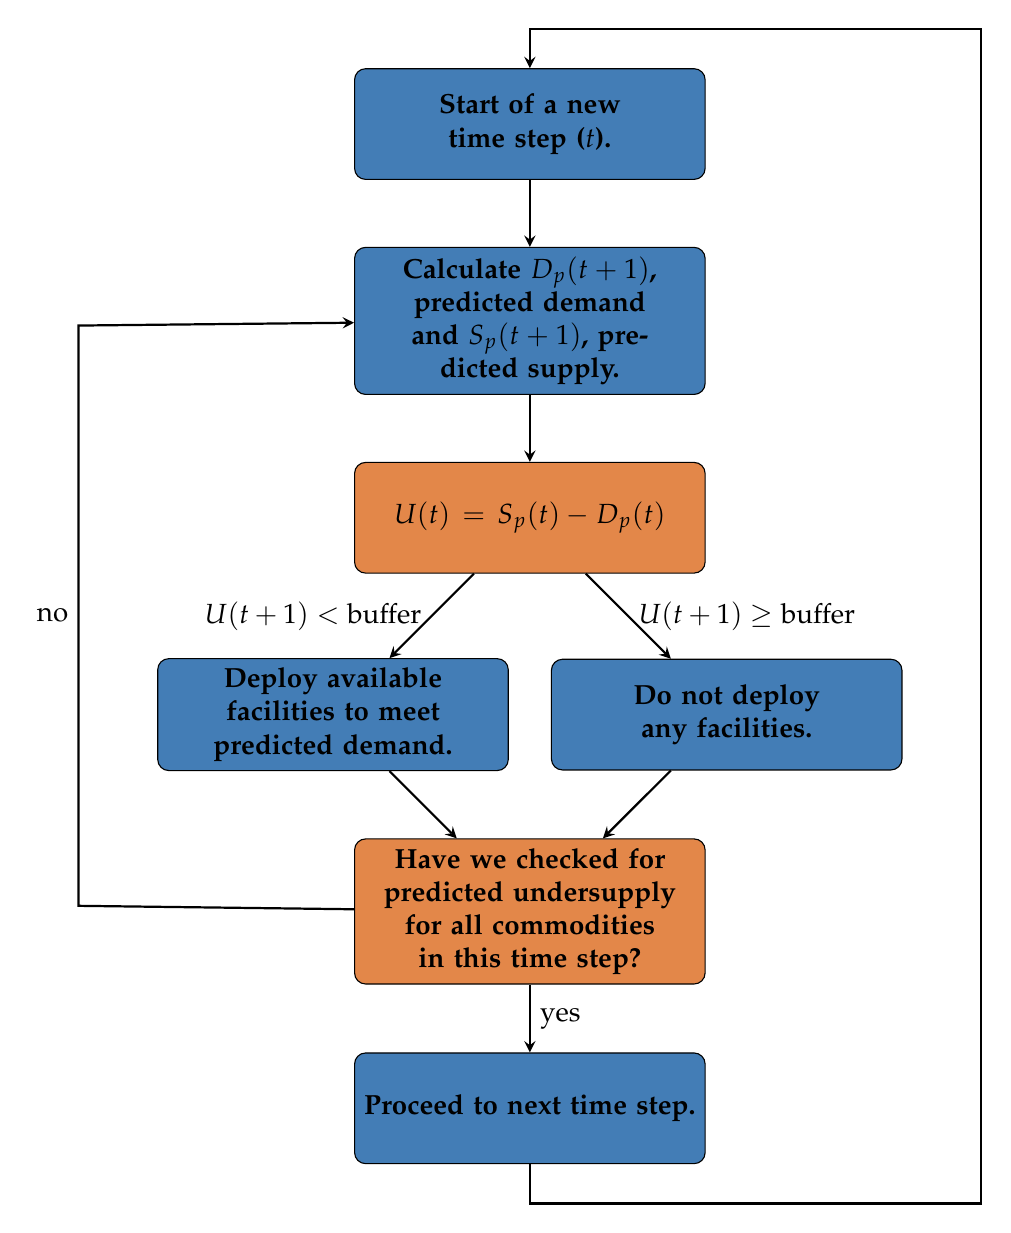
\begin{tikzpicture}[node distance=2.5cm]
	\node (Start) [bblock] {\textbf{Start of a new time step ($t$).}};
	\node (Predict) [bblock, below of=Start] {\textbf{Calculate $D_p(t+1)$, predicted demand and $S_p(t+1)$, predicted supply.}};
	\node (IsThere) [oblock, below of=Predict]{\textbf{$U(t) = S_p(t)-D_p(t)$}};
	\node (Deploy) [bblock, below of=IsThere, xshift = -2.5cm]{\textbf{Deploy available facilities to meet predicted demand.} };
    \node (NoDeploy) [bblock, right of=Deploy, xshift = 2.5cm]{\textbf{Do not deploy any facilities.} };
    \node (All) [oblock, below of=Deploy, xshift = 2.5cm] {\textbf{Have we checked for predicted undersupply for all commodities in this time step?}};
    \node (End) [bblock, below of=All] {\textbf{Proceed to next time step.}};
	
	\draw [arrow] (Start) -- (Predict); 
	\draw [arrow] (Predict) -- (IsThere);
                \draw [arrow] (IsThere) -- node[anchor=east] {$U(t+1) < \mbox{buffer}$} (Deploy);
                \draw [arrow] (IsThere) -- node[anchor=west] {$U(t+1) \geq \mbox{buffer}$} (NoDeploy);
    \draw [arrow] (Deploy) -- (All);
    \draw [arrow] (NoDeploy) -- (All);
    \draw [arrow] (All) -- node[anchor=west] {yes} (End);
    \draw [arrow] (All) -- ([shift={(-3.5cm,1cm)}]All.south west)-- node[anchor=east] {no} ([shift={(-3.5cm,-1cm)}]Predict.north west)--(Predict);
    \draw [arrow] (End) |-([shift={(3.5cm,-0.5cm)}]End.south east)-- ([shift={(3.5cm,0.5cm)}]Start.north east)-|(Start);
    \end{tikzpicture}
	\caption{\Deploy logic flow at each time step in \Cyclus. }
	\label{fig:flow}
\end{figure}

When \deploy predicts an undersupply, it responds by deploying 
the fewest number of available facilities to meet demand with minimal 
oversupply.  
This logic is available in \texttt{solver.py}. 

\subsection{\textbf{Basic User-Defined Input Variables}}
The user provides specific variables to customize their
simulation. 
Descriptions of each input variable can be found in the 
README of the \deploy github repository.

Essentially, the user must define the facilities the 
\deploy institution controls and can deploy. 
The user must also define the driving commodity, all facility capacities 
for producing that commodity, its demand 
equation, and which method predicts supply and demand. 
For example, the user can define a demand equation for power of 
$D_p(t) = 1000 t$ MW and \deploy will deploy available reactor and supporting 
facilities to meet the defined power demand at each timestep, $t$. 

The user can also provide a time-dependent equation that governs
preference for a particular facility compared to other facilities which 
provide the same commodity. 
For example, the user can define a \gls{LWR} and a \gls{SFR} to have
preferences of $p_{LWR}(t) = 101 - t$ and $p_{SFR}(t) = t$ respectively. 
The institution will prefer deployment of \gls{LWR} facilities over 
\gls{SFR} before time step 51, when $p_{SFR}(t)$ becomes greater than 
$p_{SFR}(t)$. 

The user can constrain facility deployment 
until a facility accumulates enough inventory of a specific commodity.  
The user can also define an initial facility list of facilities to be 
present in the institution at the beginning of the simulation. 

\subsection{\textbf{Prediction Algorithms}}
Three interchangeable algorithm types govern demand and supply 
predictions: non-optimizing (NO), deterministic optimizing (DO), and stochastic
optimizing (SO). 

There are three methods implemented for the non-optimizing model: 
Moving Average (MA), autoregressive moving average (ARMA), and autoregressive 
conditional heteroskedasticity (ARCH).
There are four methods implemented for the deterministic optimizing model: 
Polynomial fit regression (POLY), simple exponential smoothing (EXP\_SMOOTHING),
triple exponential smoothing (HOLT\_WINTERS) and fast fourier 
transform (FFT). 
There is one method implemented for stochastic optimizing model: 
stepwise seasonal (SW\_SEASONAL).  

The user can choose which prediction algorithm governs each specific 
\deploy commodity. 
The effectiveness of a prediction algorithm depends on the type 
of power demand in a scenario and the type of commodity (demand 
driving commodity vs non-driving commodity, demand driven 
deployment vs supply driven deployment etc.). 
For example, the most effective method
for predicting demand and supply for the power commodity in a scenario  
with a sinusoidal power demand is the triple exponential smoothing method. 
However, for the non-driving commodities in the same 
scenario, the fast fourier transform method is more effective than triple 
exponential smoothing. 
This paper will comment on these categories of problems and their suitable
algorithms. 

\subsection{\textbf{Demand-driven vs. Supply-driven Institutions}}
\Deploy defines two institutions: \texttt{DemandDrivenDeploymentInst} and \texttt{Supply-}
\noindent
\texttt{DrivenDeploymentInst}.
The prior exists for the front-end of the fuel cycle and the latter 
for the back-end. 
For example, for front end facilities, the reactor demands 
fuel and \texttt{DemandDrivenDeploymentInst} triggers the deployment 
of fuel fabrication facilities to create supply meeting the demand 
for fuel.
For back end facilities, the reactor generates spent fuel 
and \texttt{SupplyDrivenDeploymentInst} triggers the deployment of 
waste repository facilities to create capacity for storage of the supply 
of spent fuel. 

\subsection{\textbf{Installed Capacity}}
The user can choose between deploying facilities based on the difference 
between predicted demand and predicted supply or predicted demand and 
installed capacity.
Two advantages make preferable to use installed capacity over predicted 
supply. 
The first is for facilities that provide intermittent supply, such as a 
reactor facility with a designated refueling time. 
During time steps in which a reactor is refueling, the user might not 
want \deploy to deploy more facilities to make up for the lack of supply
caused by this one time step gap in supply. 
The second is for situations in which the input commodity for a facility has
run out and the facility that produces the input commodity 
is no longer commissionable. 
Therefore, with the demand for the output commodity of that facility, \deploy
would deploy that facility to meet the demand, however due to the lack of 
the input commodity, even if there are infinite numbers of that facility, 
it will not produce the output commodity. 
For example, in a transition scenario from LWRs to fast reactors, the fast 
reactor demand for Pu may exceed the inventory provided by LWRs before 
they were decommissioned. 
This will result in the deployment of mixer facilities that generate the 
fast reactor fuel despite the lack of plutonium to generate the fuel. 
This can be avoided by constraining fast reactor facility deployment 
until a sizable inventory of Pu is accumulated. 

\subsection{\textbf{Supply/Capacity Buffer}}
In \texttt{DemandDrivenDeploymentInst}, the user can choose to provide a
buffer for predicted supply.
\Deploy will deploy facilities to meet the predicted demand with the 
additional buffer. 

In \texttt{SupplyDrivenDeploymentInst}, the user can choose to 
provide a buffer for predicted capacity.
\Deploy will deploy facilities to meet the predicted supply with the 
additional buffer. 
The buffer can be defined as a percentage value (equation \ref{eq:perc}) 
or an absolute value (equation \ref{eq:abs}): 

\begin{align}
            \label{eq:perc}
        S_{pwb} &= S_{p}(1+d)\\
            \label{eq:abs}
        S_{pwb} &= S_{p}+a
\end{align}

where $S_{pwb}$ is predicted supply/capacity with buffer, 
$S_p$ is the predicted supply/capacity without buffer, 
$d$ is the percentage value in decimal form, 
and $a$ is the absolute value of the buffer. 

\section{Demonstration of d3ploy capabilities}
Constant, linearly increasing, and sinusoidal power demand simulations
are shown to demonstrate \deploy's capabilities. 
A balance between the various system parameters must be 
met for each type of simulation to meet the goal of 
minimizing undersupply and under capacity for the various 
commodities. 
The input files and scripts to produce the plots in this paper 
can be reproduced using \cite{d3ploy_doi_2019}.

These simulations are basic transition scenarios that only include
three types of facilities: \texttt{source}, \texttt{reactor} and 
\texttt{sink}.
All simulations in this work begin with a ten reactor facilities, 
\texttt{reactor1} to \texttt{reactor10}. 
These reactors have staggered cycle lengths and lifetimes 
so that they do not all refuel and decommission at the same time 
steps. 
When the ten initial reactor facilities begin to decommission, 
\deploy deploys reactor facilities of \texttt{newreactor} type
to meet unmet demand for power. 
All the simulations deploy facilities based on the relationship
between predicted demand and installed capacity. 
This capability was discussed in the previous section.  
Table \ref{tab:transition-scenario-all} shows the simulation 
parameters that are consistent across all the discussed 
scenarios. 

\begin{table}[!htb]
    \centering
    \caption {Transition scenario parameters that are consisted for constant, linear increasing and sinusoidal power demand simulations}
	\label{tab:transition-scenario-all}
        \begin{tabularx}{0.8\textwidth}{lX}
    \hline
    \textbf{Parameters}    & \textbf{Description} \\ \hline
    Facilities Present     & \texttt{Source} (Capacity: 3000kg)\\
                & \texttt{Reactor} (Capacity: 1000MW)\\
                & \texttt{Sink} (Capacity: 50000kg)      \\ 
                \hline
    New Reactor Parameters & Cycle time: 18\\
                & Refuel time: 1\\
                \hline
    Driving Commodity & Power \\ \hline
    \end{tabularx}
\end{table}

These basic transition scenarios were set up to 
demonstrate \deploy's capabilities for simulating 
transition scenarios and 
to inform decisions about input parameters when setting up larger 
demand transition scenarios with many facilities. 

\subsection{Transition Scenario: Constant Demand}

In this section, a constant power transition scenario is shown. 
Table \ref{tab:transition-scenario-constant-power} shows the 
simulation parameters used in this transition scenario.  
The input file used to generate this simulation can be found in 
\href{https://github.com/arfc/d3ploy/blob/master/input/constant_transition.xml}{constant\_transition.xml} 
and the file used to run the simulation and generate the plots can be found in 
\href{https://github.com/arfc/d3ploy/blob/master/tests/performance_tests/algorithm_performance_tests_transitions.py}{algorithm\_performance\_tests\_transitions.py}.

\begin{table}[!htb]
    \centering
    \caption{Constant Power Demand Transition Scenario Parameters}
	\label{tab:transition-scenario-constant-power}
        \begin{tabularx}{\textwidth}{l|lX}
    \hline
        \textbf{Commodity} & \textbf{Parameter}    & \textbf{Description} \\ \hline
                \textbf{Power}& Demand Equation & $D_p(t) = 10000 MW$ \\ \hline
    \multirow{2}{*}{\textbf{Power}} & Prediction Method      &  Fast Fourier Transform\\
                                     & Supply Buffer          &  3000 MW \\ \hline
    \multirow{2}{*}{\textbf{Fuel}}  & Prediction Method      &  Moving Average\\
                                     & Supply Buffer & 0 kg \\ \hline
    \multirow{2}{*}{\textbf{\shortstack{Spent Fuel}}}  & Prediction Method      &  Moving Average\\
                                     & Capacity Buffer & 0 kg \\ \hline
        \end{tabularx}
\end{table}

Figures \ref{fig:constanttransition-power}, \ref{fig:constanttransition-fuel}
and \ref{fig:constanttransition-spentfuel} demonstrate \deploy's capability 
to deploy reactor and supporting facilities to meet the user 
determined power demand and subsequently demanded secondary commodities 
with minimal undersupply. 
Table \ref{tab:transition-scenario-results} shows the number of 
undersupplied time steps. 

\begin{table}[htb]
    \centering
    \caption{Undersupply results for each commodity in each scenario}
	\label{tab:transition-scenario-results}
        \begin{tabularx}{\textwidth}{l|lR}
    \hline
    \textbf{Power Demand Equation}    & \textbf{Commodity}    & \textbf{Undersupplied Time Steps} \\ \hline
    \multirow{2}{*}{\textbf{Constant}} & Fuel & 1 \\ 
                                             & Power & 0 \\ 
                                             & Spent Fuel & 0 \\ \hline
    \multirow{2}{*}{\textbf{\shortstack{Linearly Increasing}}} & Fuel & 1 \\ 
                                             & Power & 0 \\ 
                                             & Spent Fuel & 0 \\ \hline
    \multirow{2}{*}{\textbf{Sinusoidal}} & Fuel & 1 \\ 
                                             & Power & 1 \\ 
                                             & Spent Fuel & 0 \\ \hline
    \end{tabularx}
\end{table}

In figure \ref{fig:constanttransition-power}, the supply of power never falls under demand.
By using a combination of the fast fourier transform method for predicting 
demand and setting the supply buffer to 3000MW (the capacity of 3 reactors), 
the user minimizes the number of undersupplied time steps of every commodity. 
To avoid an undersupply, it is helpful to perform a
sensitivity analysis of the size 
of buffer to use for each commodity. 

In figure \ref{fig:constanttransition-fuel},
a facility with a large fuel throughput is initially
deployed to meet the large initial fuel demand for the starting
up of ten reactors. 
\Deploy is prevented from deploying many supporting
facilities that end up being redundant at the later parts of 
the simulation, by having an initial facility with a large throughput
exist for the first few time steps in the simulation.
This is a reflection of reality in which reactor manufacturers will 
accumulate an appropriate amount of fuel inventory before starting 
up reactors. 
After the decommissioning of the large initial fuel production facility
we notice an undersypply in one time step.
This is unavoidable since the prediction methods in \deploy are 
unable to predict this sudden drop in demand. 

\begin{figure*}[!htbp]
    \centering
    \begin{subfigure}[t]{\textwidth}
    \centering
        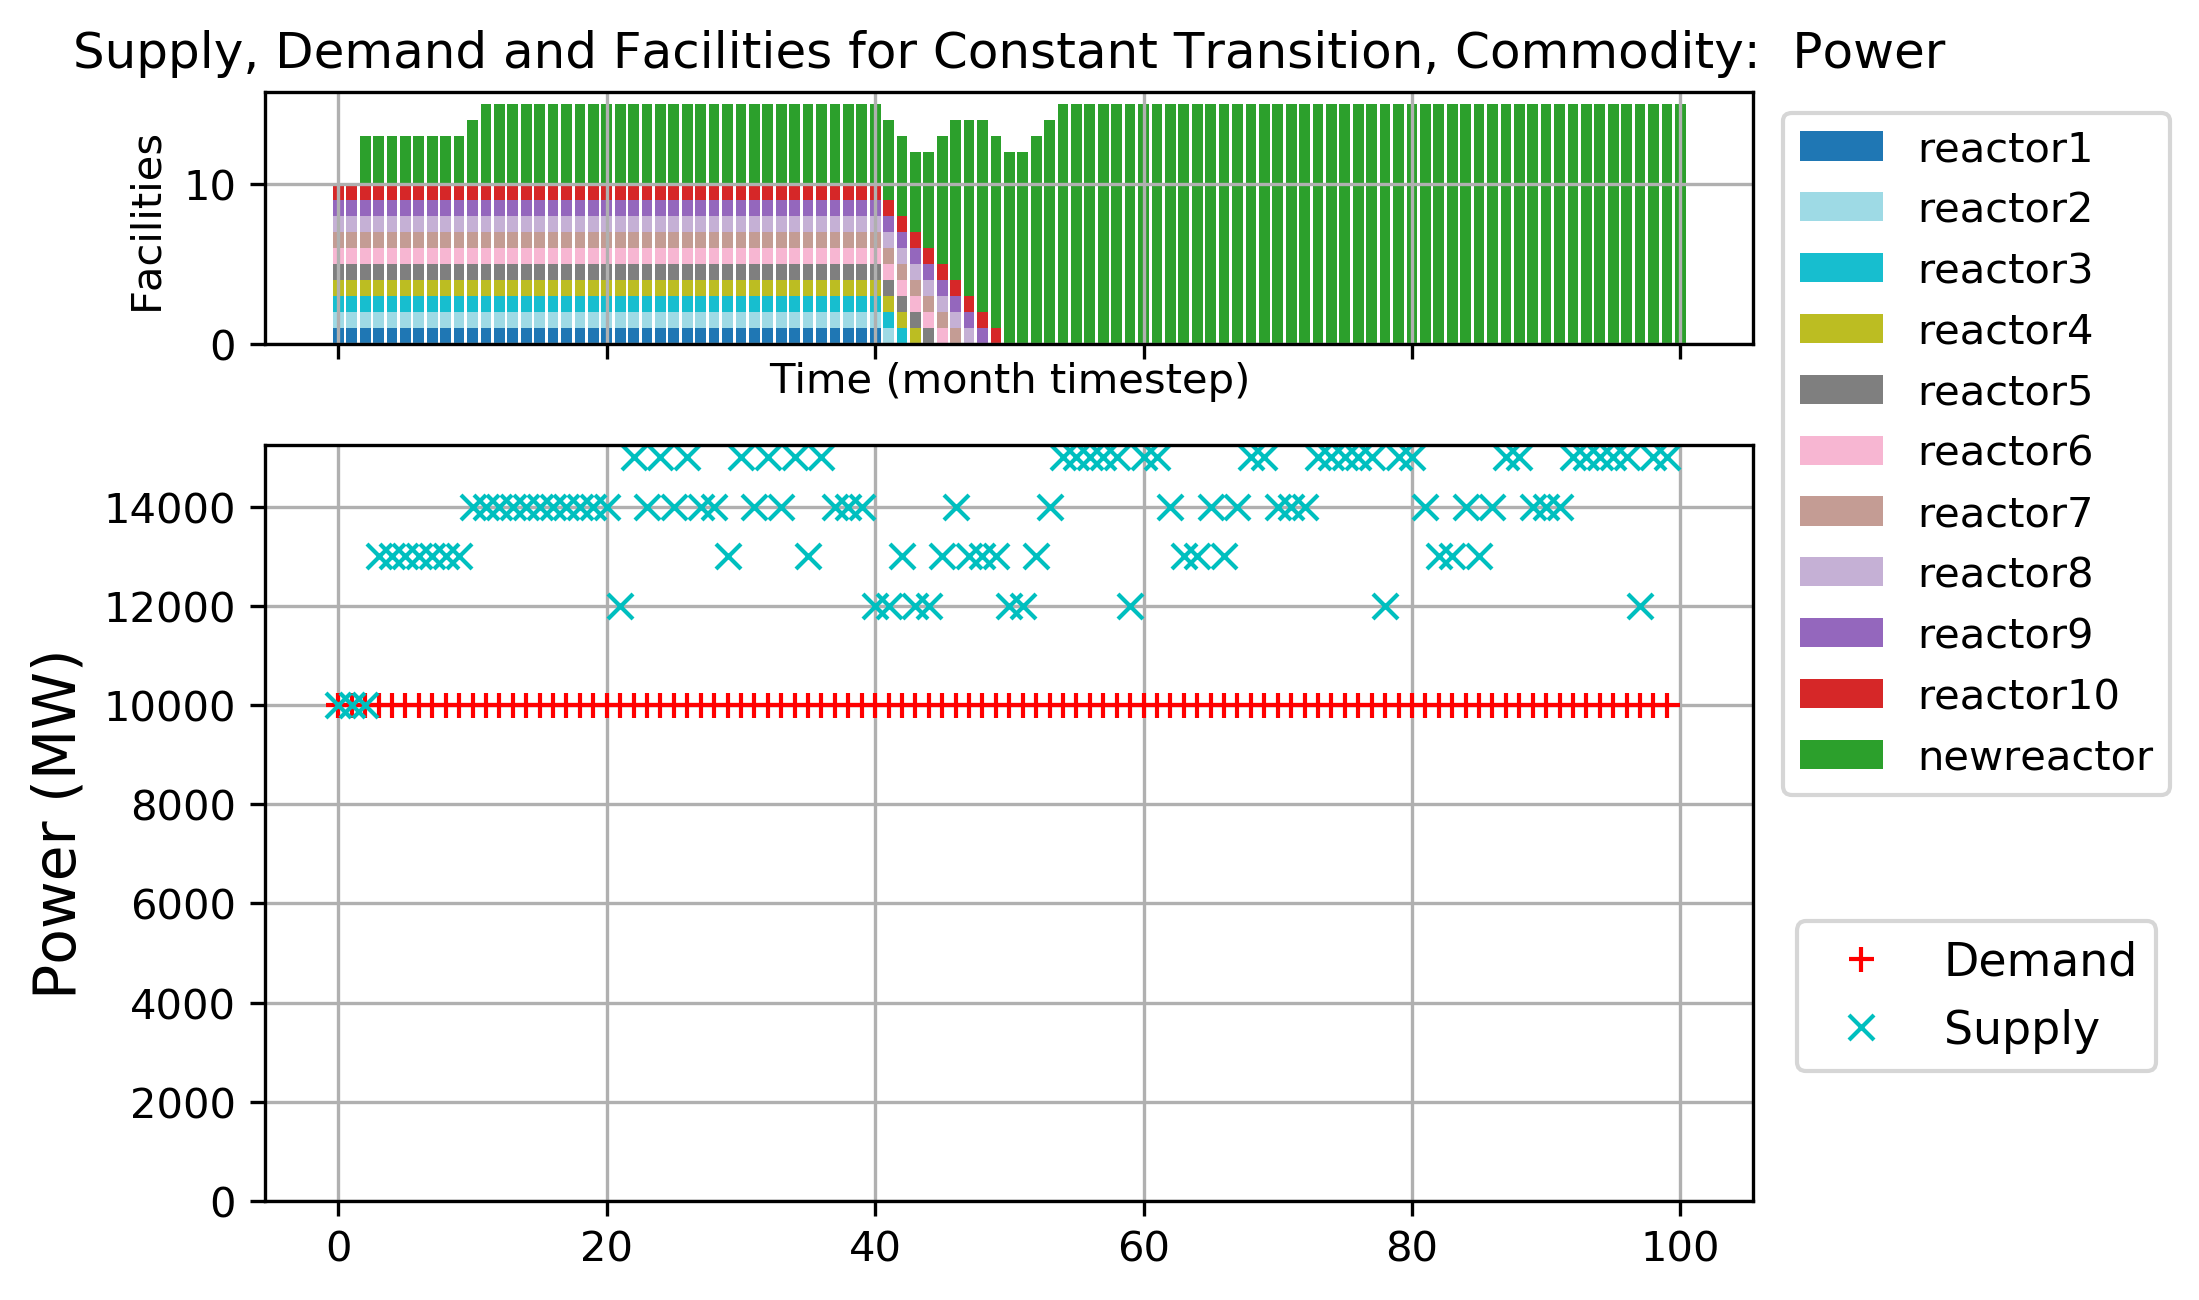
\includegraphics[width=0.8\linewidth]{figures/constanttransition-power.png} 
        \caption{The power demand is a user-defined equation and power is supplied by the reactors.}
        \label{fig:constanttransition-power}
    \end{subfigure}
    \begin{subfigure}[t]{\textwidth}
        \centering
        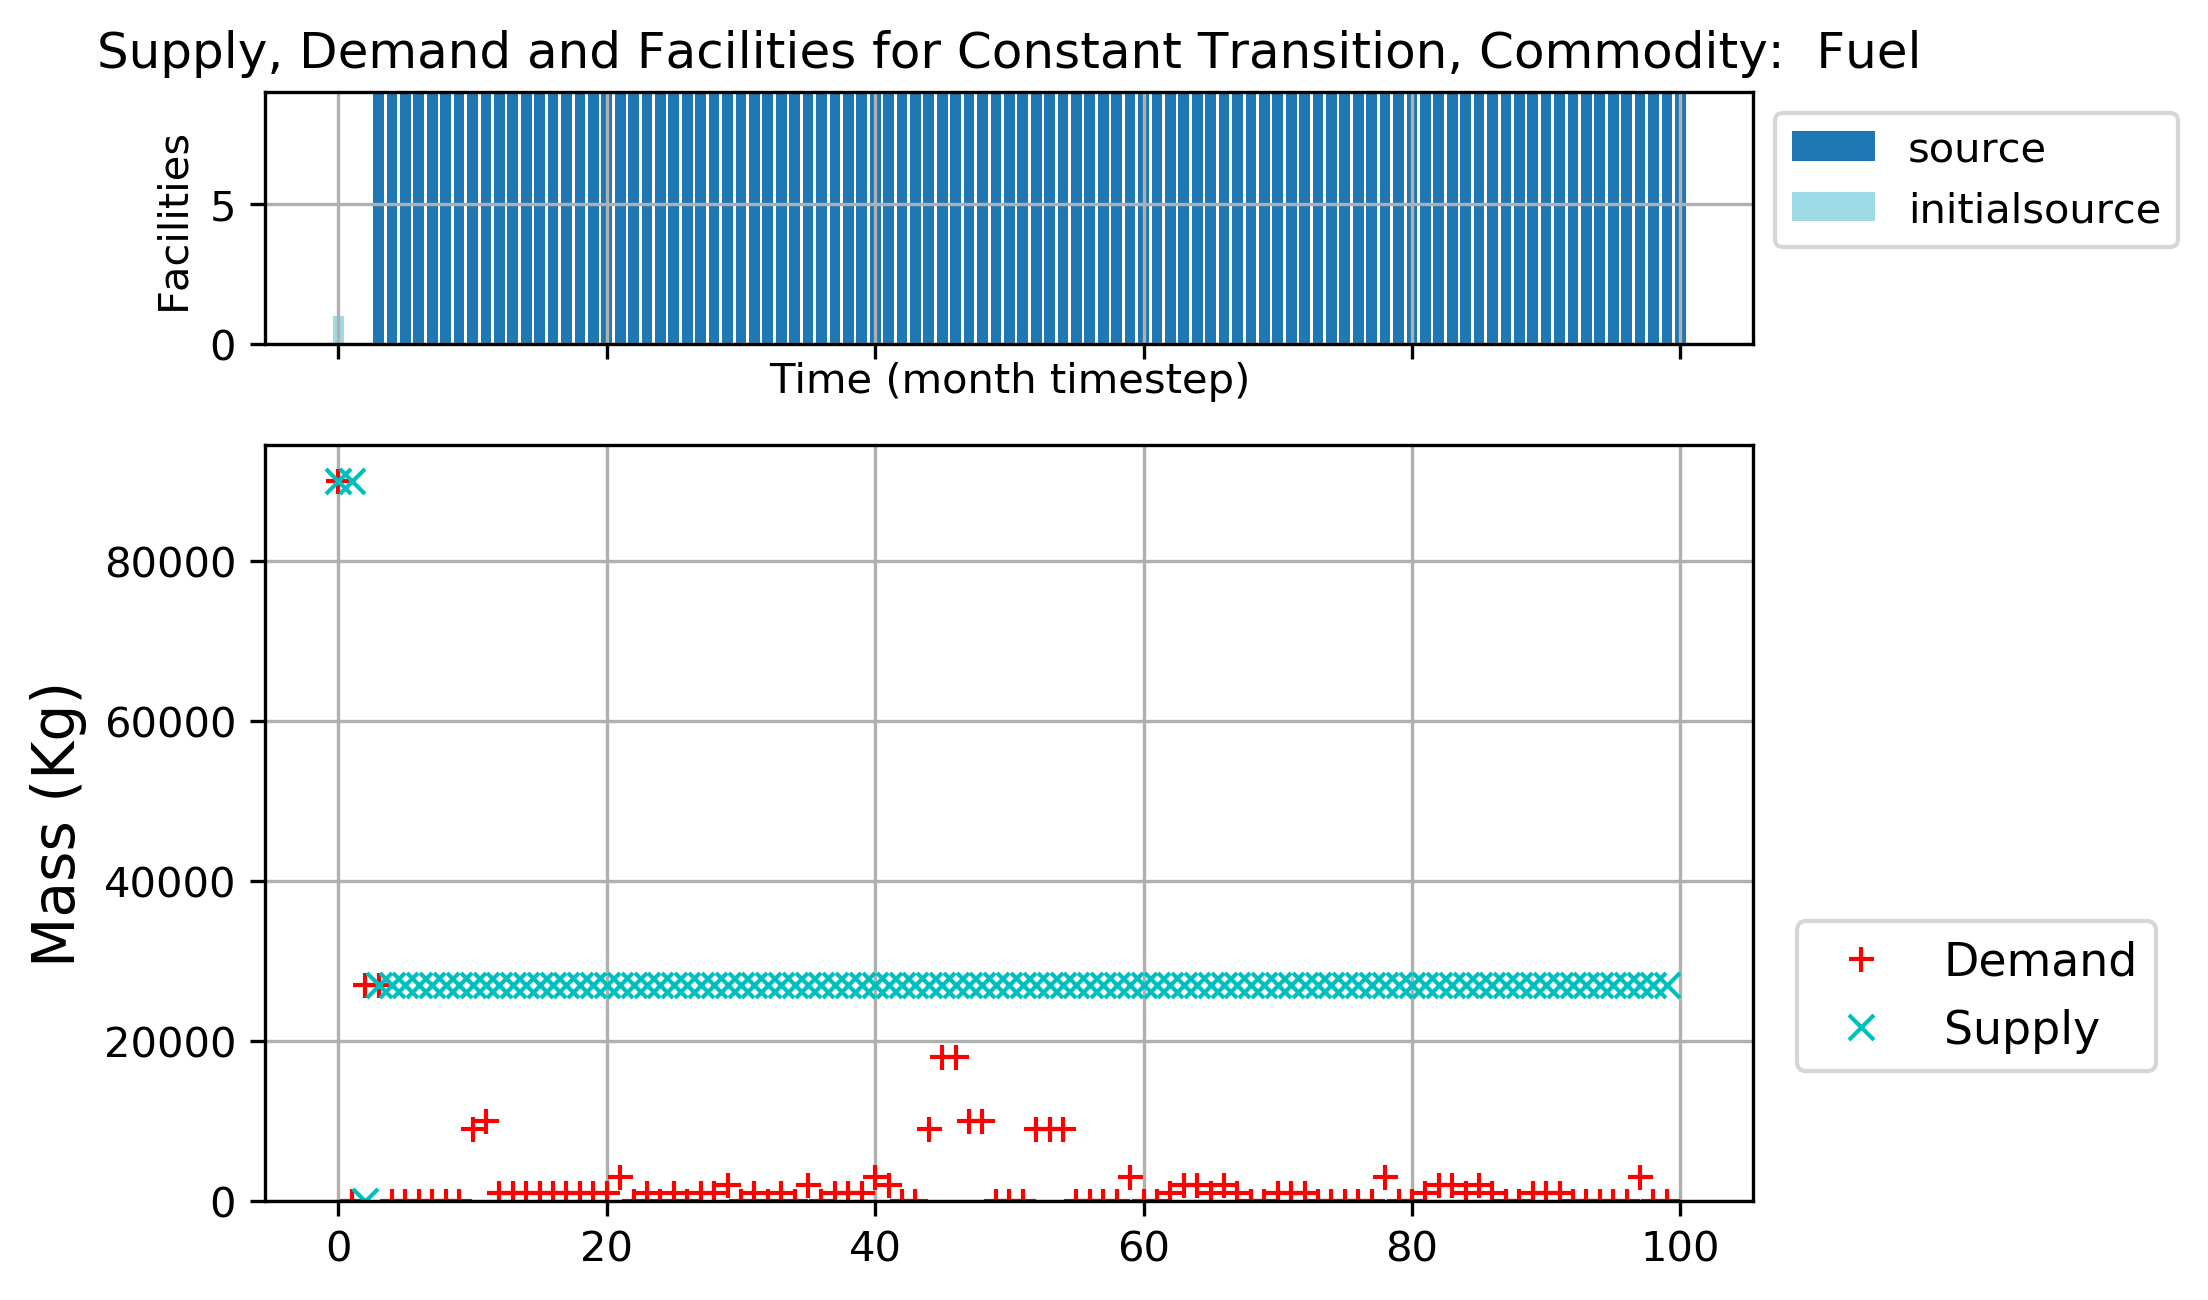
\includegraphics[width=0.8\linewidth]{figures/constanttransition-fuel.png} 
        \caption{Fuel is demanded by reactors and supplied by source facilities.}
	    \label{fig:constanttransition-fuel}
    \end{subfigure}
    \begin{subfigure}[t]{\textwidth}
        \centering
        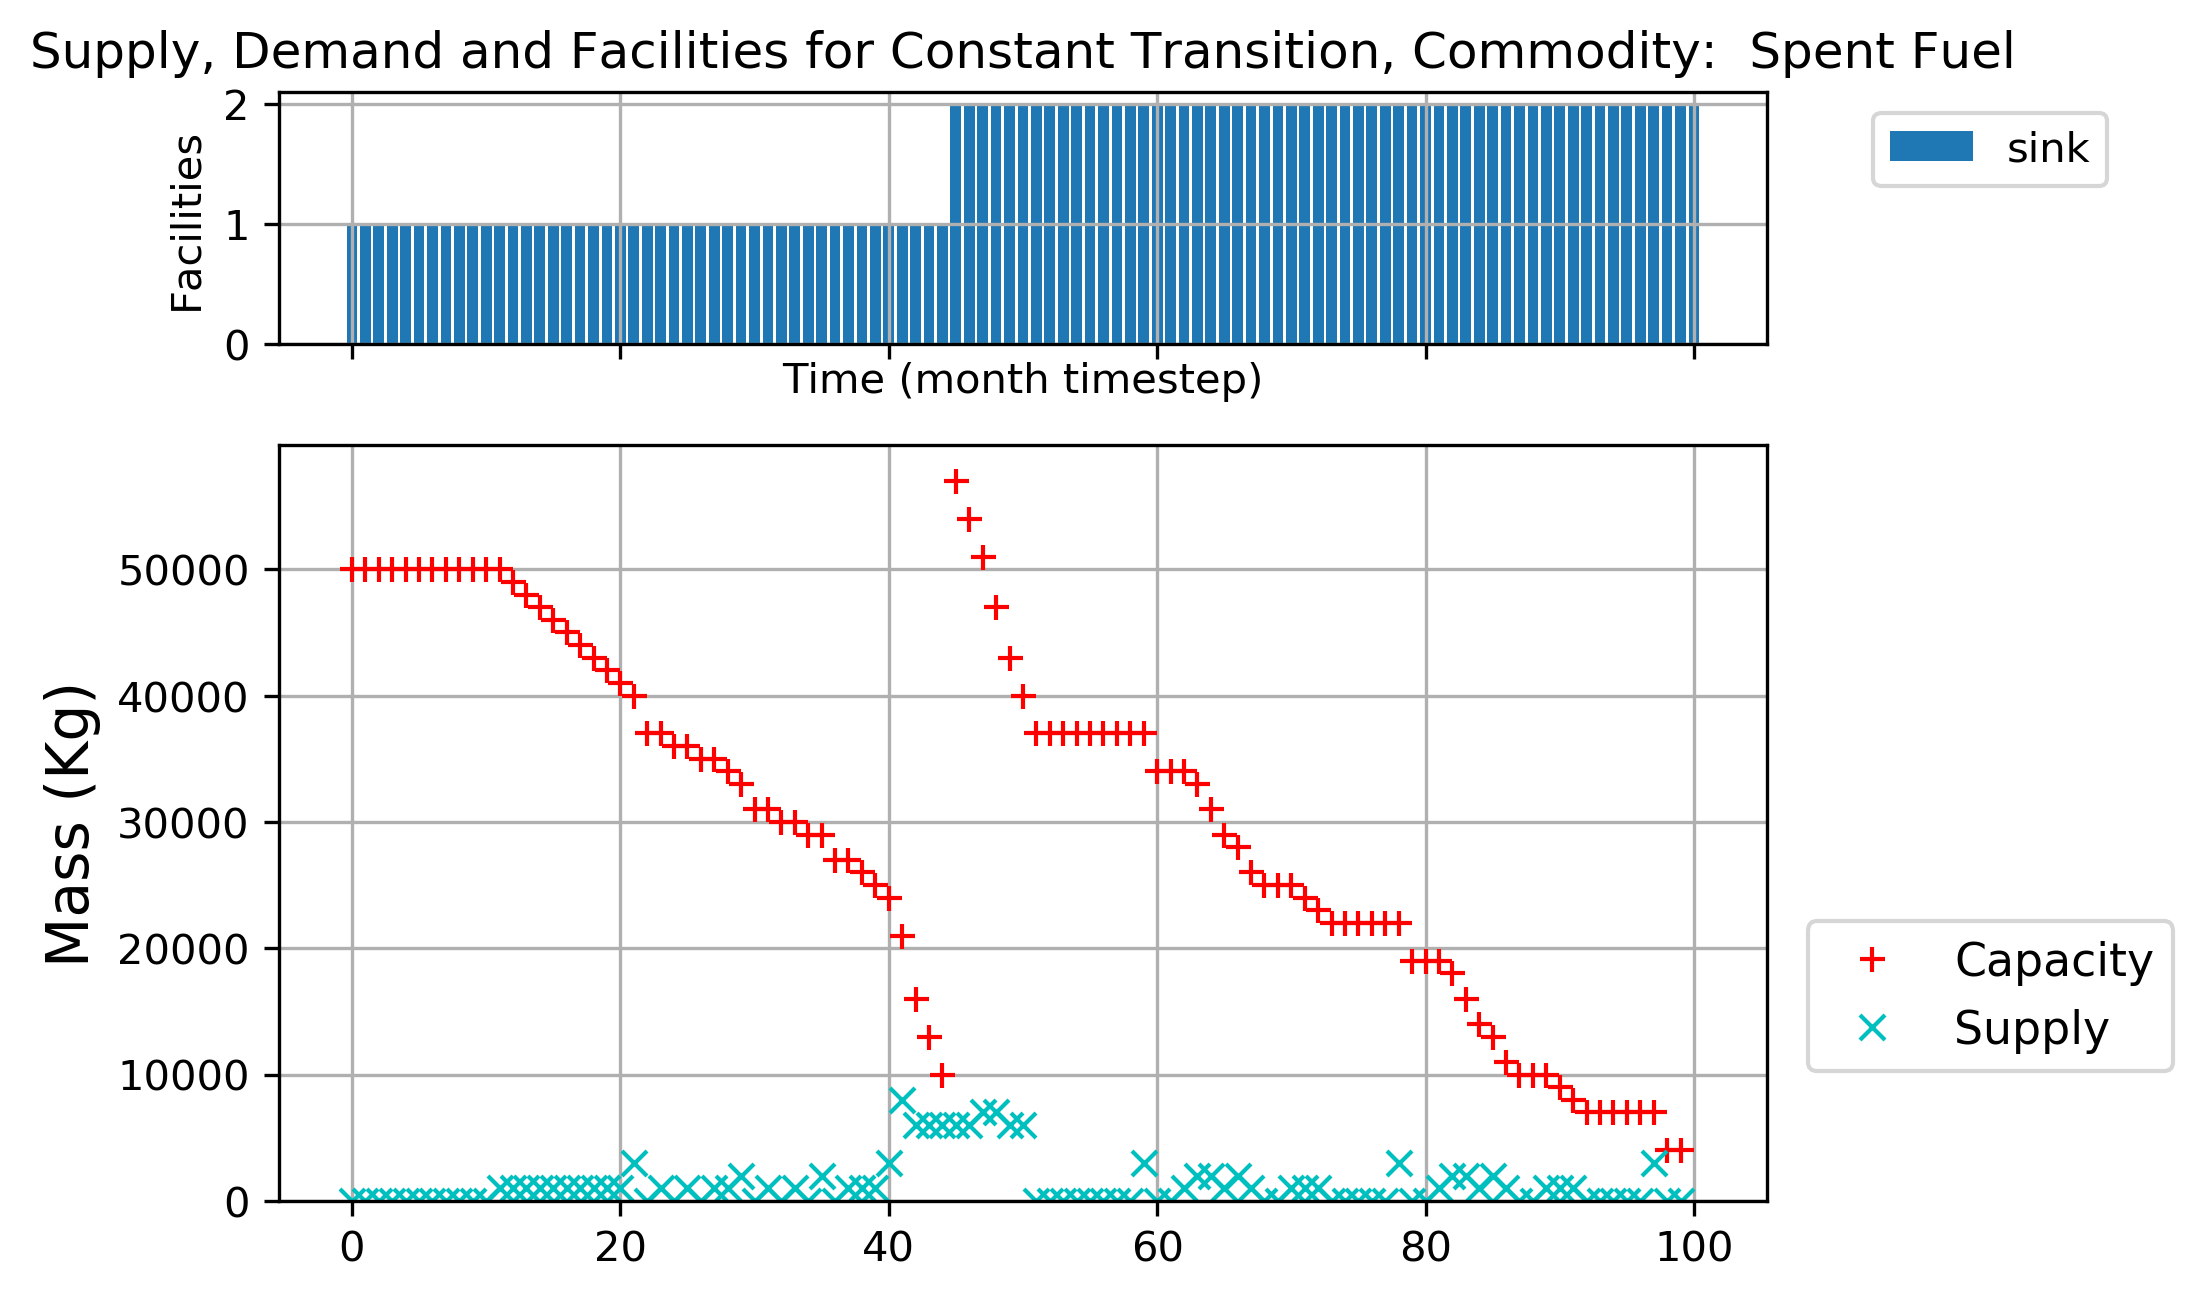
\includegraphics[width=0.8\linewidth]{figures/constanttransition-spentfuel.png} 
        \caption{Spent Fuel is supplied by reactors and the capacity is provided by sink facilities.}
        \label{fig:constanttransition-spentfuel}
    \end{subfigure}
    \caption{Transition Scenario: Constant Power Demand of 10000MW}
\end{figure*}

It is helpful to perform a small sensitivity analysis of the size 
of buffer used for each commodity to ensure that no 
undersupply occurs based on the nuances of any given facility type: 
refueling in a reactor, etc.. 
For these kind of simulations, those in which a facility requires a large initial amount of some
commodity, the user should add an initial
facility with a large production capacity that exists for only the first few time steps
in the simulation; this prevents \deploy from deploying a large number
of supporting facilities that end up being redundant later in
the simulation.
Alternatively, this could be circumvented by introducing decommissioning 
capability into \deploy.  

\subsection{Transition Scenario: Linearly Increasing Demand}

In this section, a transition scenario with a linearly 
increasing power demand is shown. 
Table \ref{tab:transition-scenario-growing-power} shows the 
simulation parameters used in this transition scenario. 

\begin{table}[!htbp]
    \centering
    \caption{Linearly Increasing Power Demand Transition Scenario Parameters}
	\label{tab:transition-scenario-growing-power}
        \begin{tabularx}{\textwidth}{l|lX}
    \hline
     \textbf{Commodity}     & \textbf{Parameter}    & \textbf{Description} \\ \hline
                \textbf{Power}& Demand Equation & $D_p(t < 40) =10000$ MW\\
                              & & $D_p(t > 40) =  250t$ MW \\ \hline
    \multirow{2}{*}{\textbf{Power}} & Prediction Method      &  Fast Fourier Transform \\  
                                     & Supply Buffer          &  2000 MW \\\hline
    \multirow{2}{*}{\textbf{Fuel}}  & Prediction Method      &  Moving Average\\ 
                                     & Supply Buffer & 1000 kg \\ \hline
    \multirow{2}{*}{\textbf{\shortstack{Spent Fuel}}}  & Prediction Method      &  Fast Fourier Transform \\ 
                                     & Capacity Buffer & 0 kg \\ \hline
    \end{tabularx}
\end{table}

Figures \ref{fig:growingtransition-power}, \ref{fig:growingtransition-fuel}
and \ref{fig:growingtransition-spentfuel} demonstrate the capability 
of \deploy to deploy reactor and supporting facilities to meet the
power demand and subsequently demanded secondary commodities 
for a linearly increasing power demand. 

The fast fourier transform method for predicting power demand is used for 
this scenario
which is identical to what was used for the constant power demand 
transition scenario. 
A smaller power buffer of 2000MW could be used while still 
minimizing under supply. 

The input file used to generate this simulation can be found in
\href{https://github.com/arfc/d3ploy/blob/master/input/growning_transition.xml}{growing\_transition.xml} 
and the file used to run the simulation and generate the plots can be found in
\href{https://github.com/arfc/d3ploy/blob/master/tests/performance_tests/algorithm_performance_tests_transitions.py}{algorithm\_performance\_tests\_transitions.py}.

\begin{figure*}[!htbp]
    \centering
    \begin{subfigure}[t]{\textwidth}
    \centering
        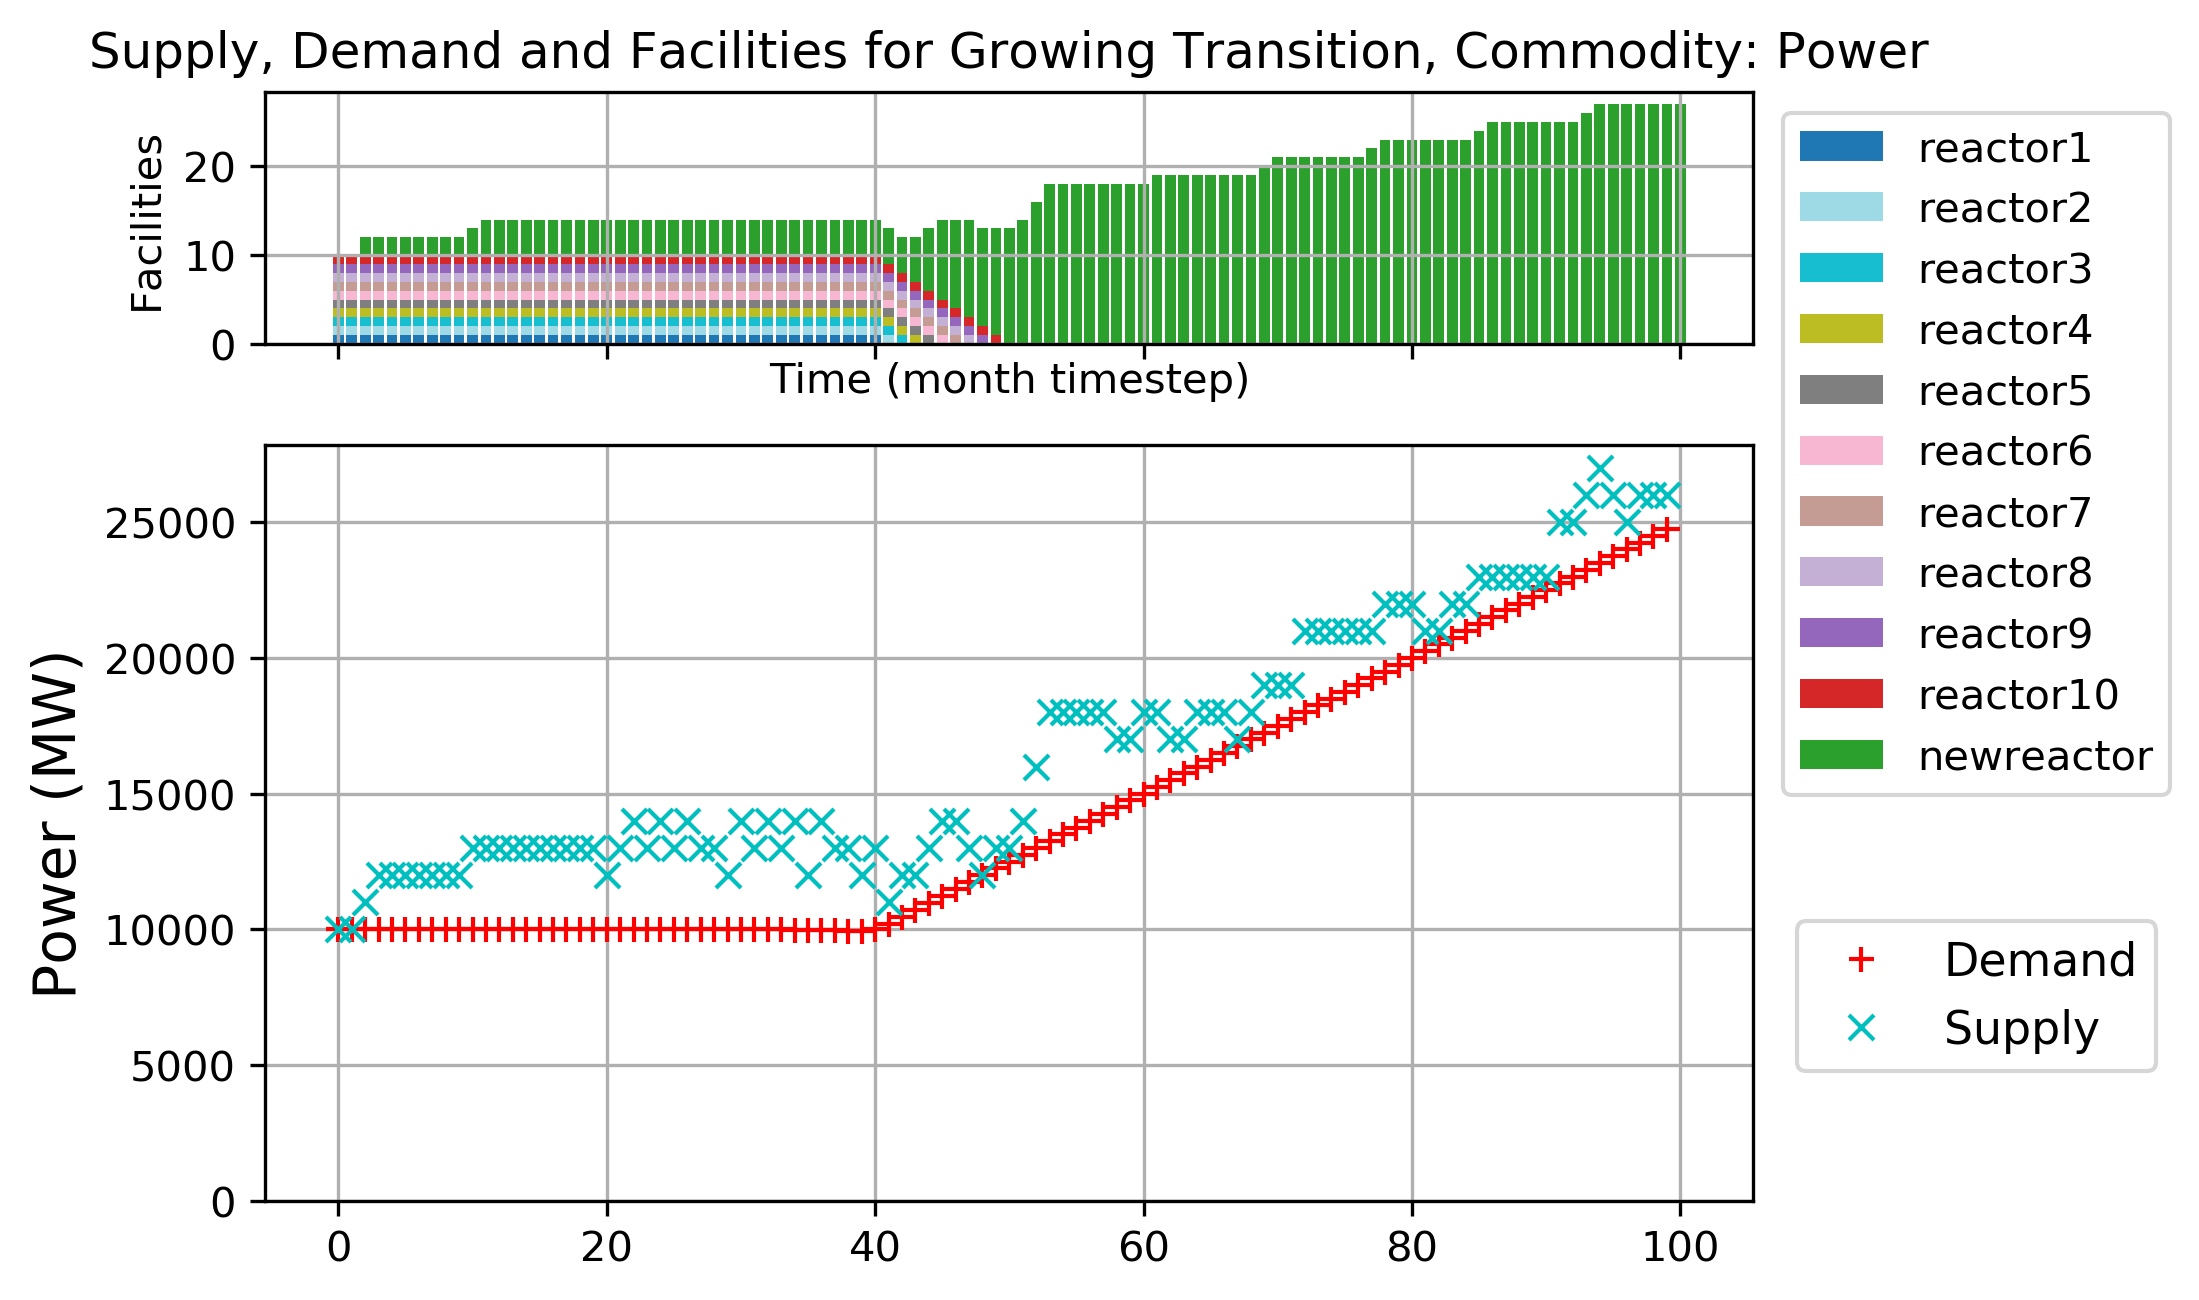
\includegraphics[width=0.8\linewidth]{figures/growingtransition-power.png} 
        \caption{The power demand is a user-defined equation and power is supplied by the reactors.}
        \label{fig:growingtransition-power}
    \end{subfigure}
    \begin{subfigure}[t]{0.65\textwidth}
        \centering
        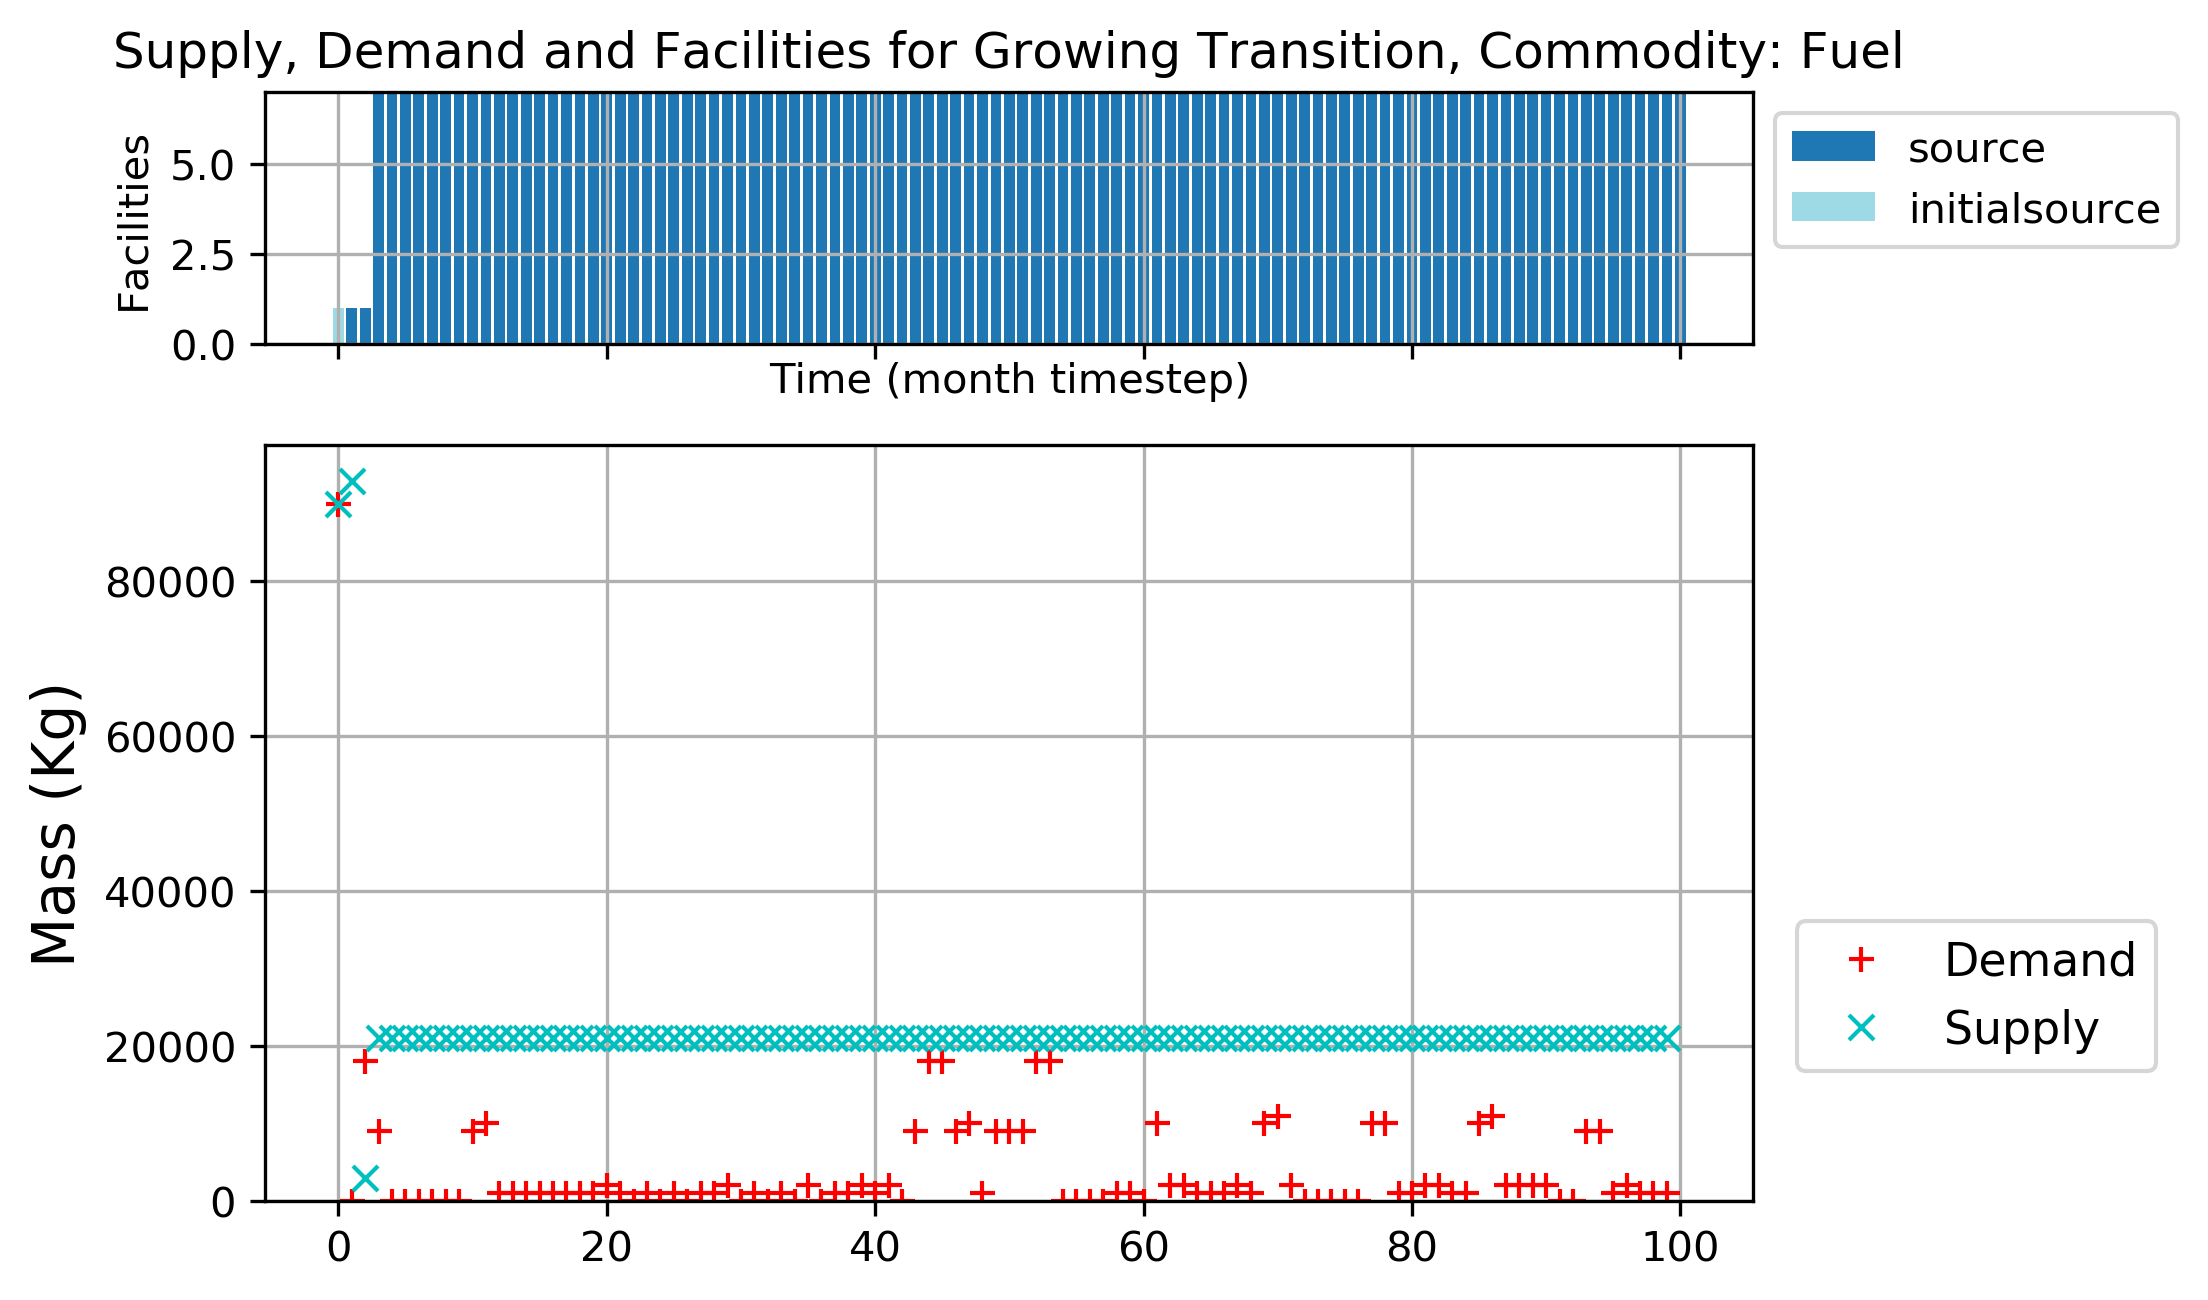
\includegraphics[width=\linewidth]{figures/growingtransition-fuel.png} 
        \caption{Fuel is demanded by reactors and supplied by source facilities.}
	    \label{fig:growingtransition-fuel}
    \end{subfigure}
    \begin{subfigure}[t]{0.65\textwidth}
        \centering
        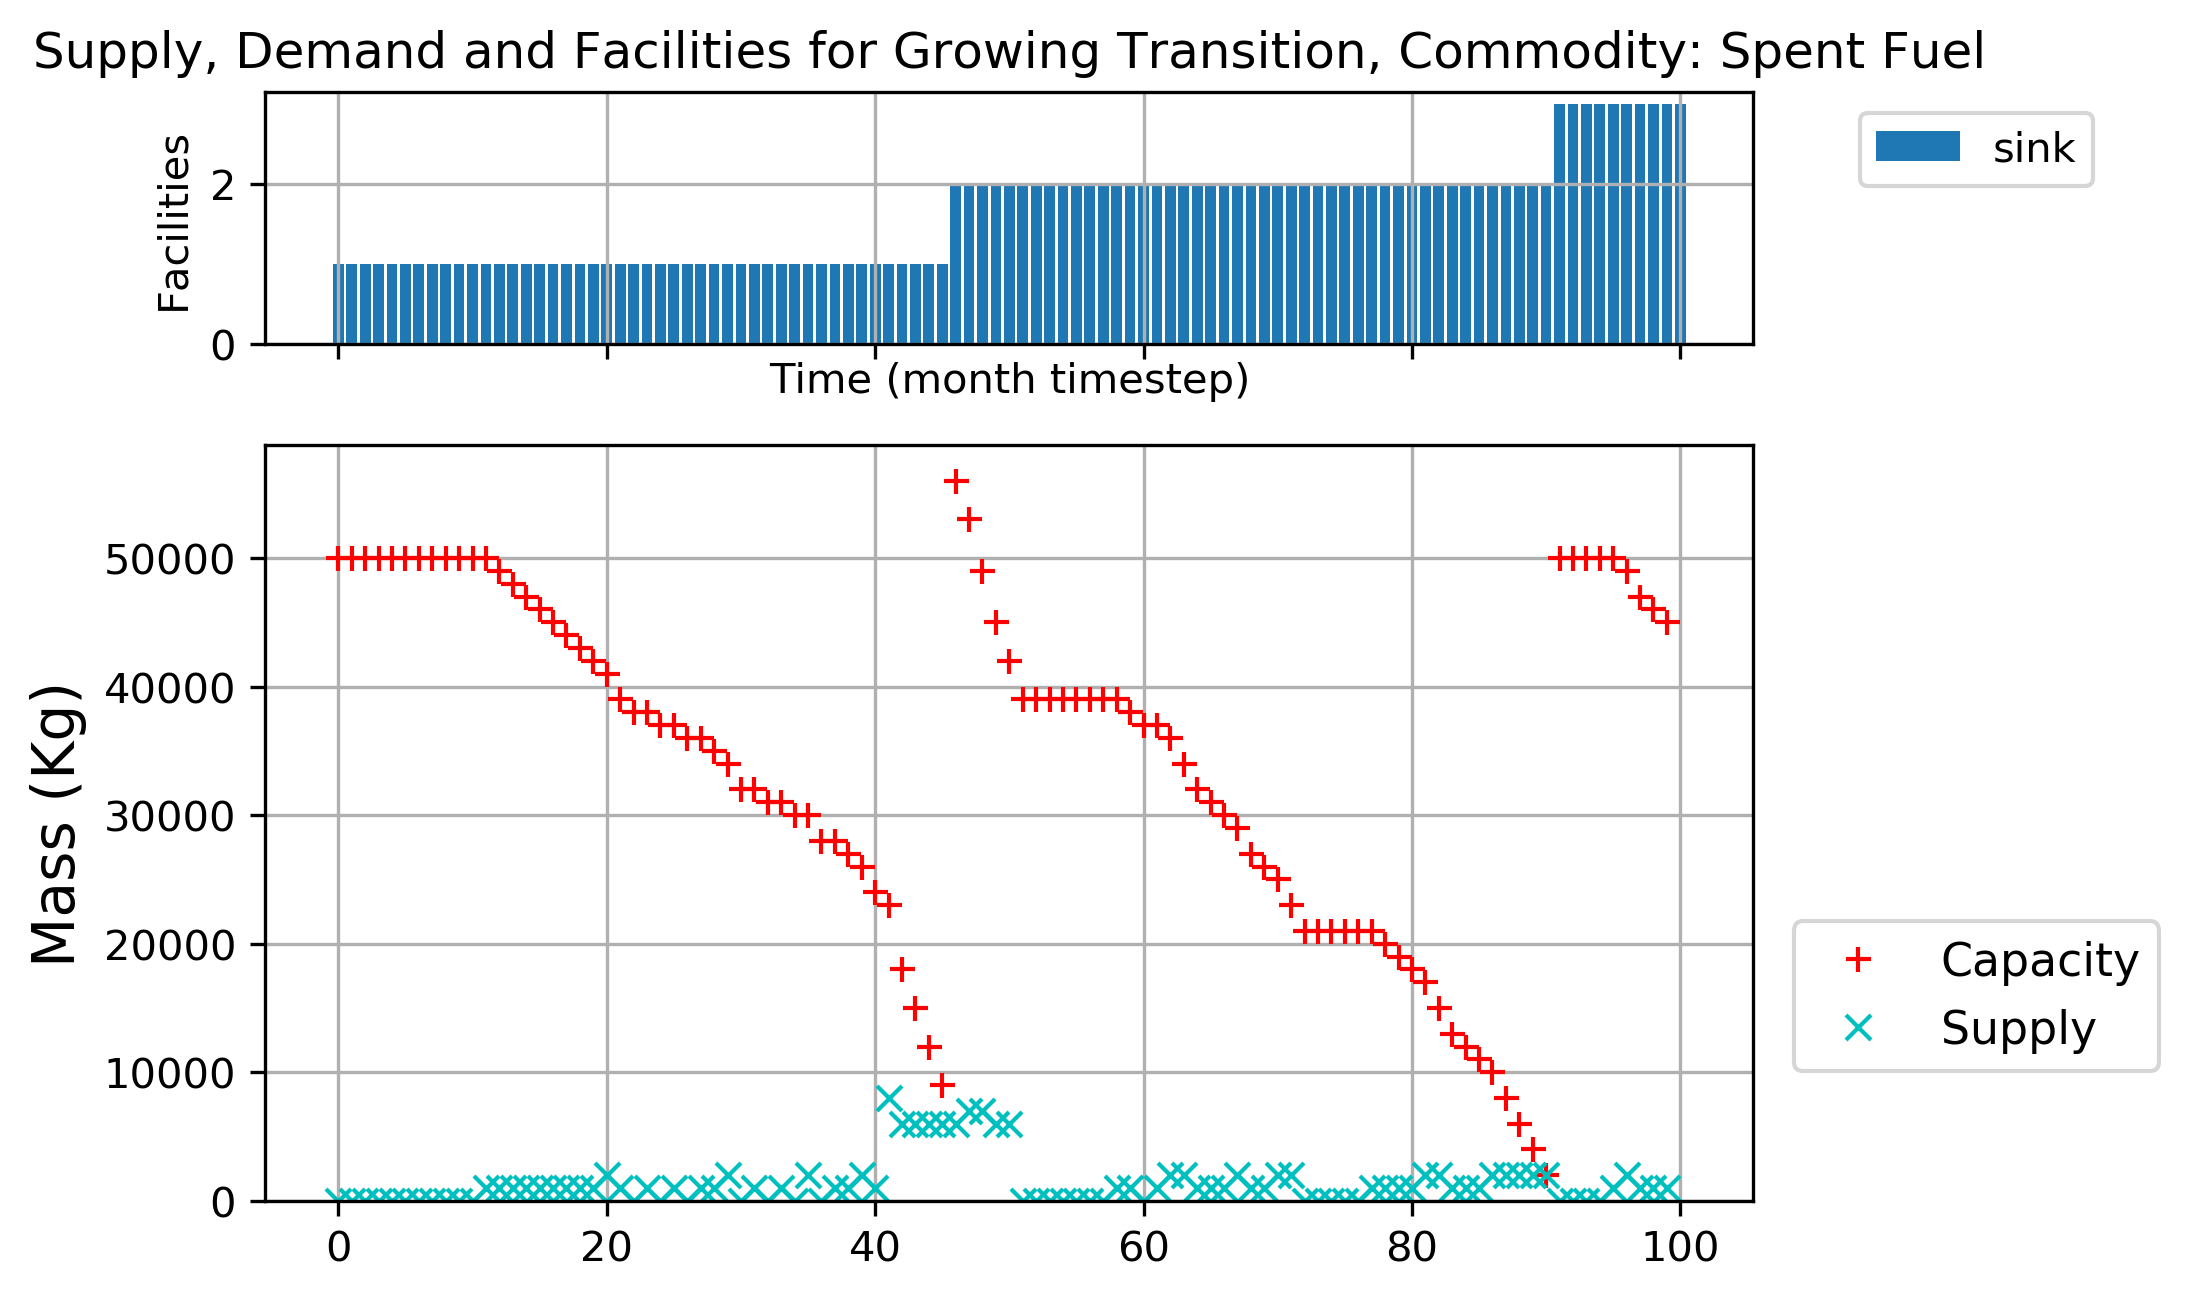
\includegraphics[width=\linewidth]{figures/growingtransition-spentfuel.png} 
        \caption{Spent Fuel is supplied by reactors and the capacity is provided by sink facilities.}
        \label{fig:growingtransition-spentfuel}
    \end{subfigure}
    \caption{Transition Scenario: Linearly increasing power demand.}
\end{figure*}

\subsection{\textbf{Transition Scenario: Sinusoidal Demand}}
In this section, a transition scenario with sinusoidal
power demand is shown. 
A sinusoidal power demand is the reflection of power demand in 
the real world such that power usage is higher in the winter and summer

and lower in the spring and fall. 
Table \ref{tab:transition-scenario-sine-power} shows the 
simulation parameters used in this transition scenario. 

Figures \ref{fig:sinetransition-power}, \ref{fig:sinetransition-fuel}
and \ref{fig:sinetransition-spentfuel} demonstrate the capability 
of \deploy to deploy reactor and supporting facilities to meet the
power demand and subsequently demanded secondary commodities 
for a sinusoidal power demand. 

For a sinusoidal power demand, the use of the triple exponential method
for predicting demand is more effective than the 
fast fourier transform method which was used for the constant 
and linearly increasing power demand transition scenarios. 
This is because the triple exponential smoothing method excels in
forecasting data points for repetitive seasonal series of data.  

\begin{table}[!htp]
    \caption {Sinusoidal Power Demand Transition Scenario Parameters}
	\label{tab:transition-scenario-sine-power}
        \begin{tabularx}{\textwidth}{l|lX}
    \hline
        \textbf{Commodity}    & \textbf{Parameter}    & \textbf{Description} \\ \hline
                \textbf{Power}& Demand Equation & $D_p(t) = 1000\sin{\left(\frac{\pi t}{3}\right)}+10000$ \\ \hline
    \multirow{2}{*}{\textbf{Power }} & Prediction Method      &  Triple Exponential Smoothing \\  
                                     & Supply Buffer          &  2000 MW (2 reactor capacities)\\ \hline
    \multirow{2}{*}{\textbf{Fuel}}  & Prediction Method      &  Moving Average\\ 
                                     & Supply Buffer & 1000 kg \\ \hline
    \multirow{2}{*}{\textbf{\shortstack{Spent Fuel}}}  & Prediction Method      & Fast Fourier Transform\\ 
                                     & Capacity Buffer & 0 kg \\ \hline
    \end{tabularx}
\end{table}

The input file used to generate this simulation can be found in:
\href{https://github.com/arfc/d3ploy/blob/master/input/sine_transition.xml}{sine\_transition.xml} 
and the file used to run the simulation and generate the plots can be found in:
\href{https://github.com/arfc/d3ploy/blob/master/tests/performance_tests/algorithm_performance_tests_transitions.py}{algorithm\_performance\_tests\_transitions.py}.

\begin{figure*}[!htbp]
    \centering
    \begin{subfigure}[t]{\textwidth}
    \centering
        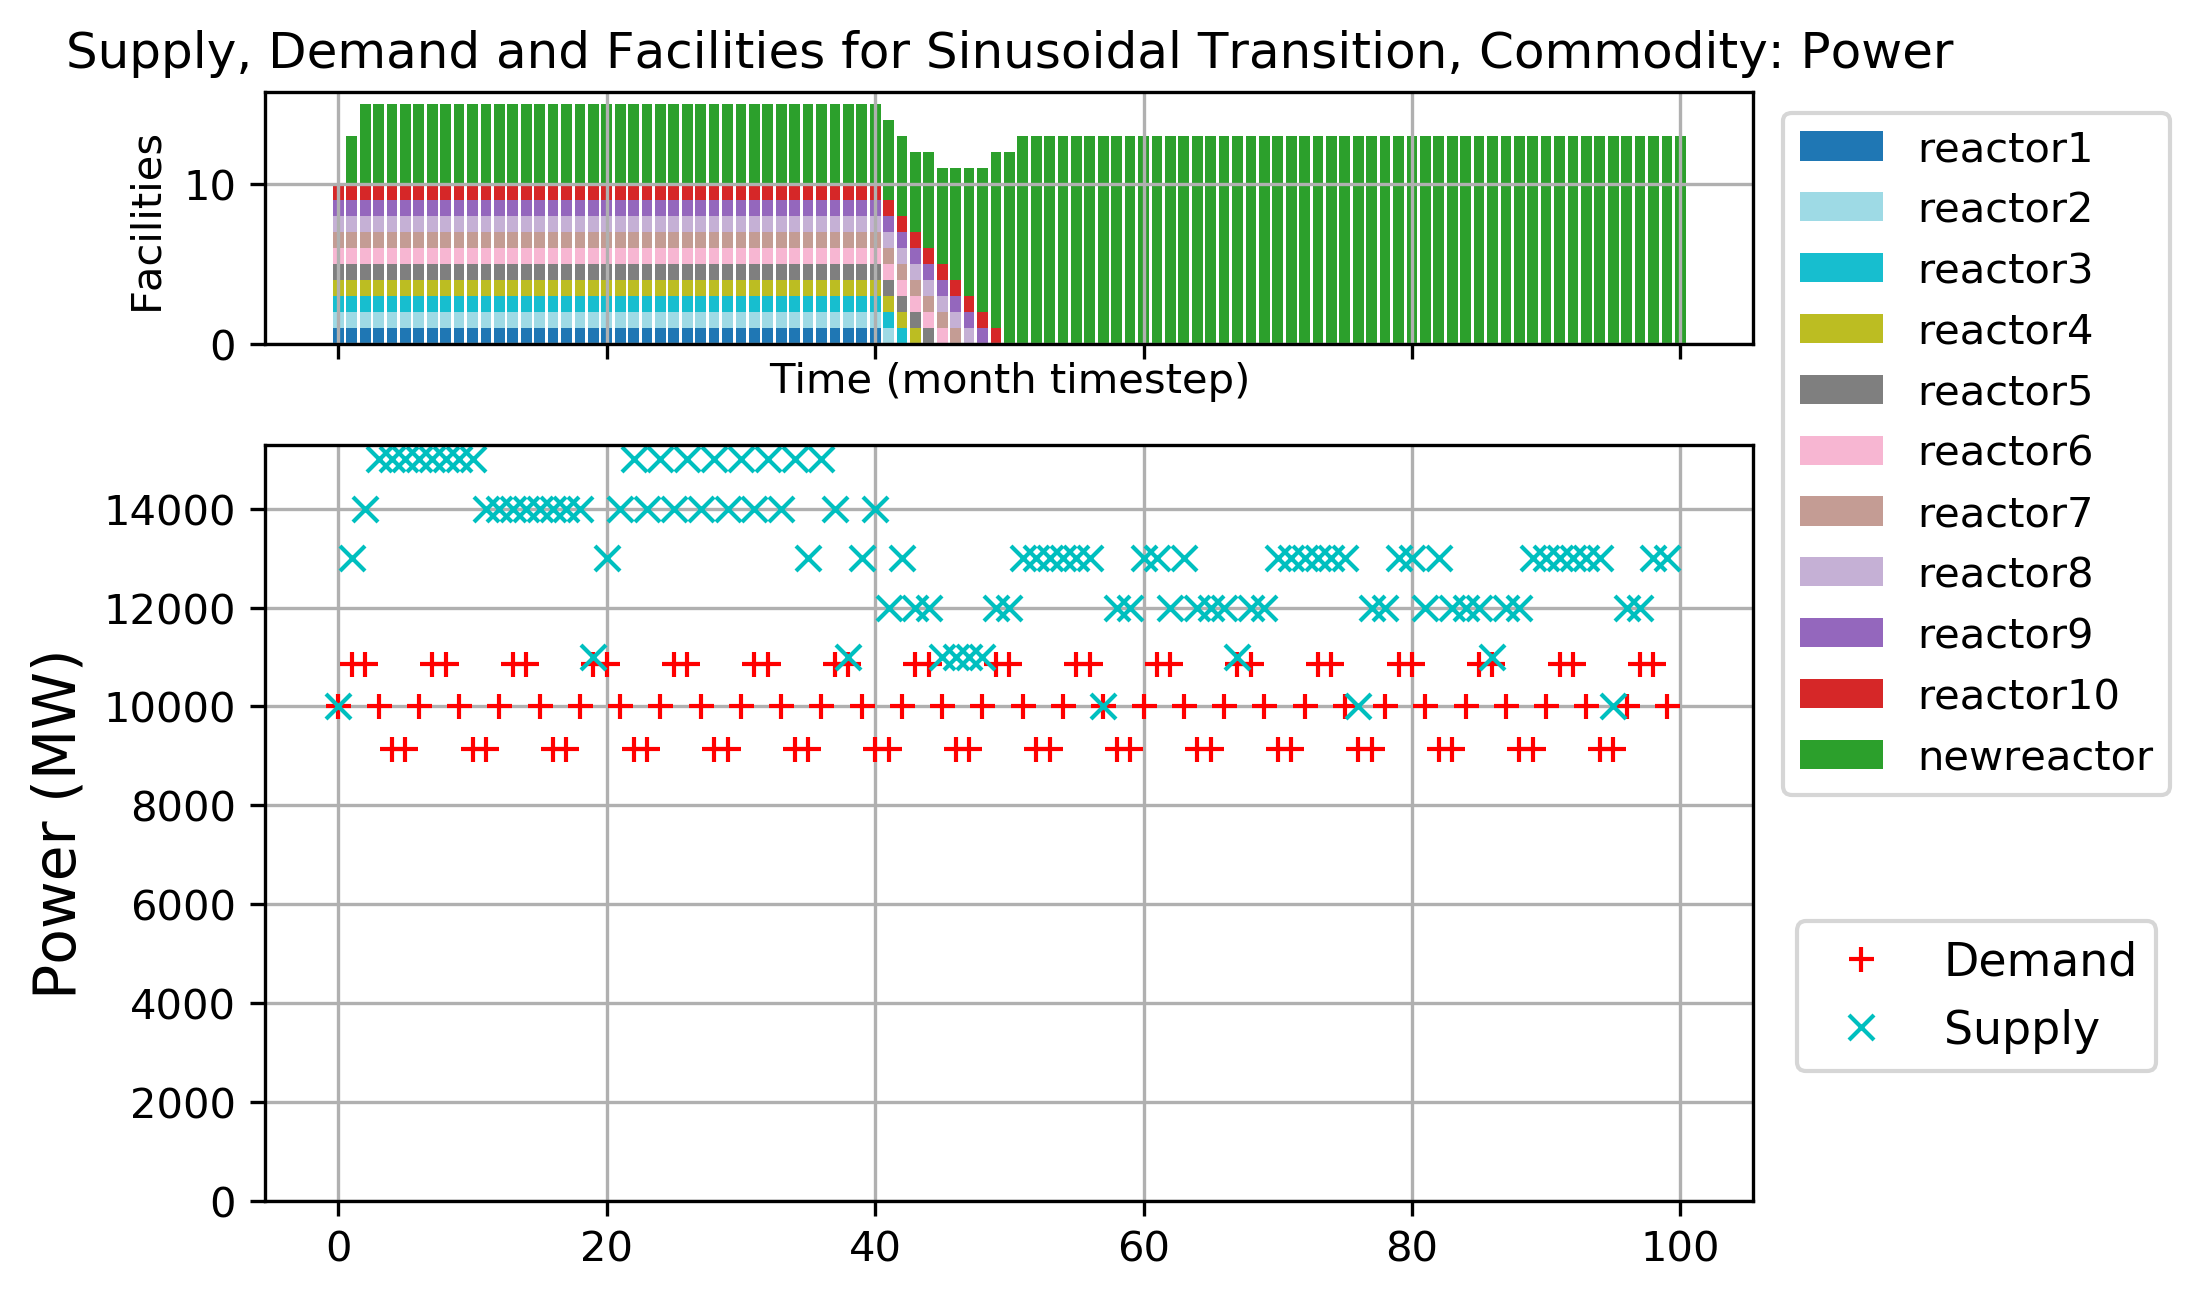
\includegraphics[width=0.8\linewidth]{figures/sinetransition-power.png} 
        \caption{The power demand is a user-defined equation and power is supplied by the reactors.}
        \label{fig:sinetransition-power}
    \end{subfigure}
    \begin{subfigure}[t]{0.65\textwidth}
        \centering
        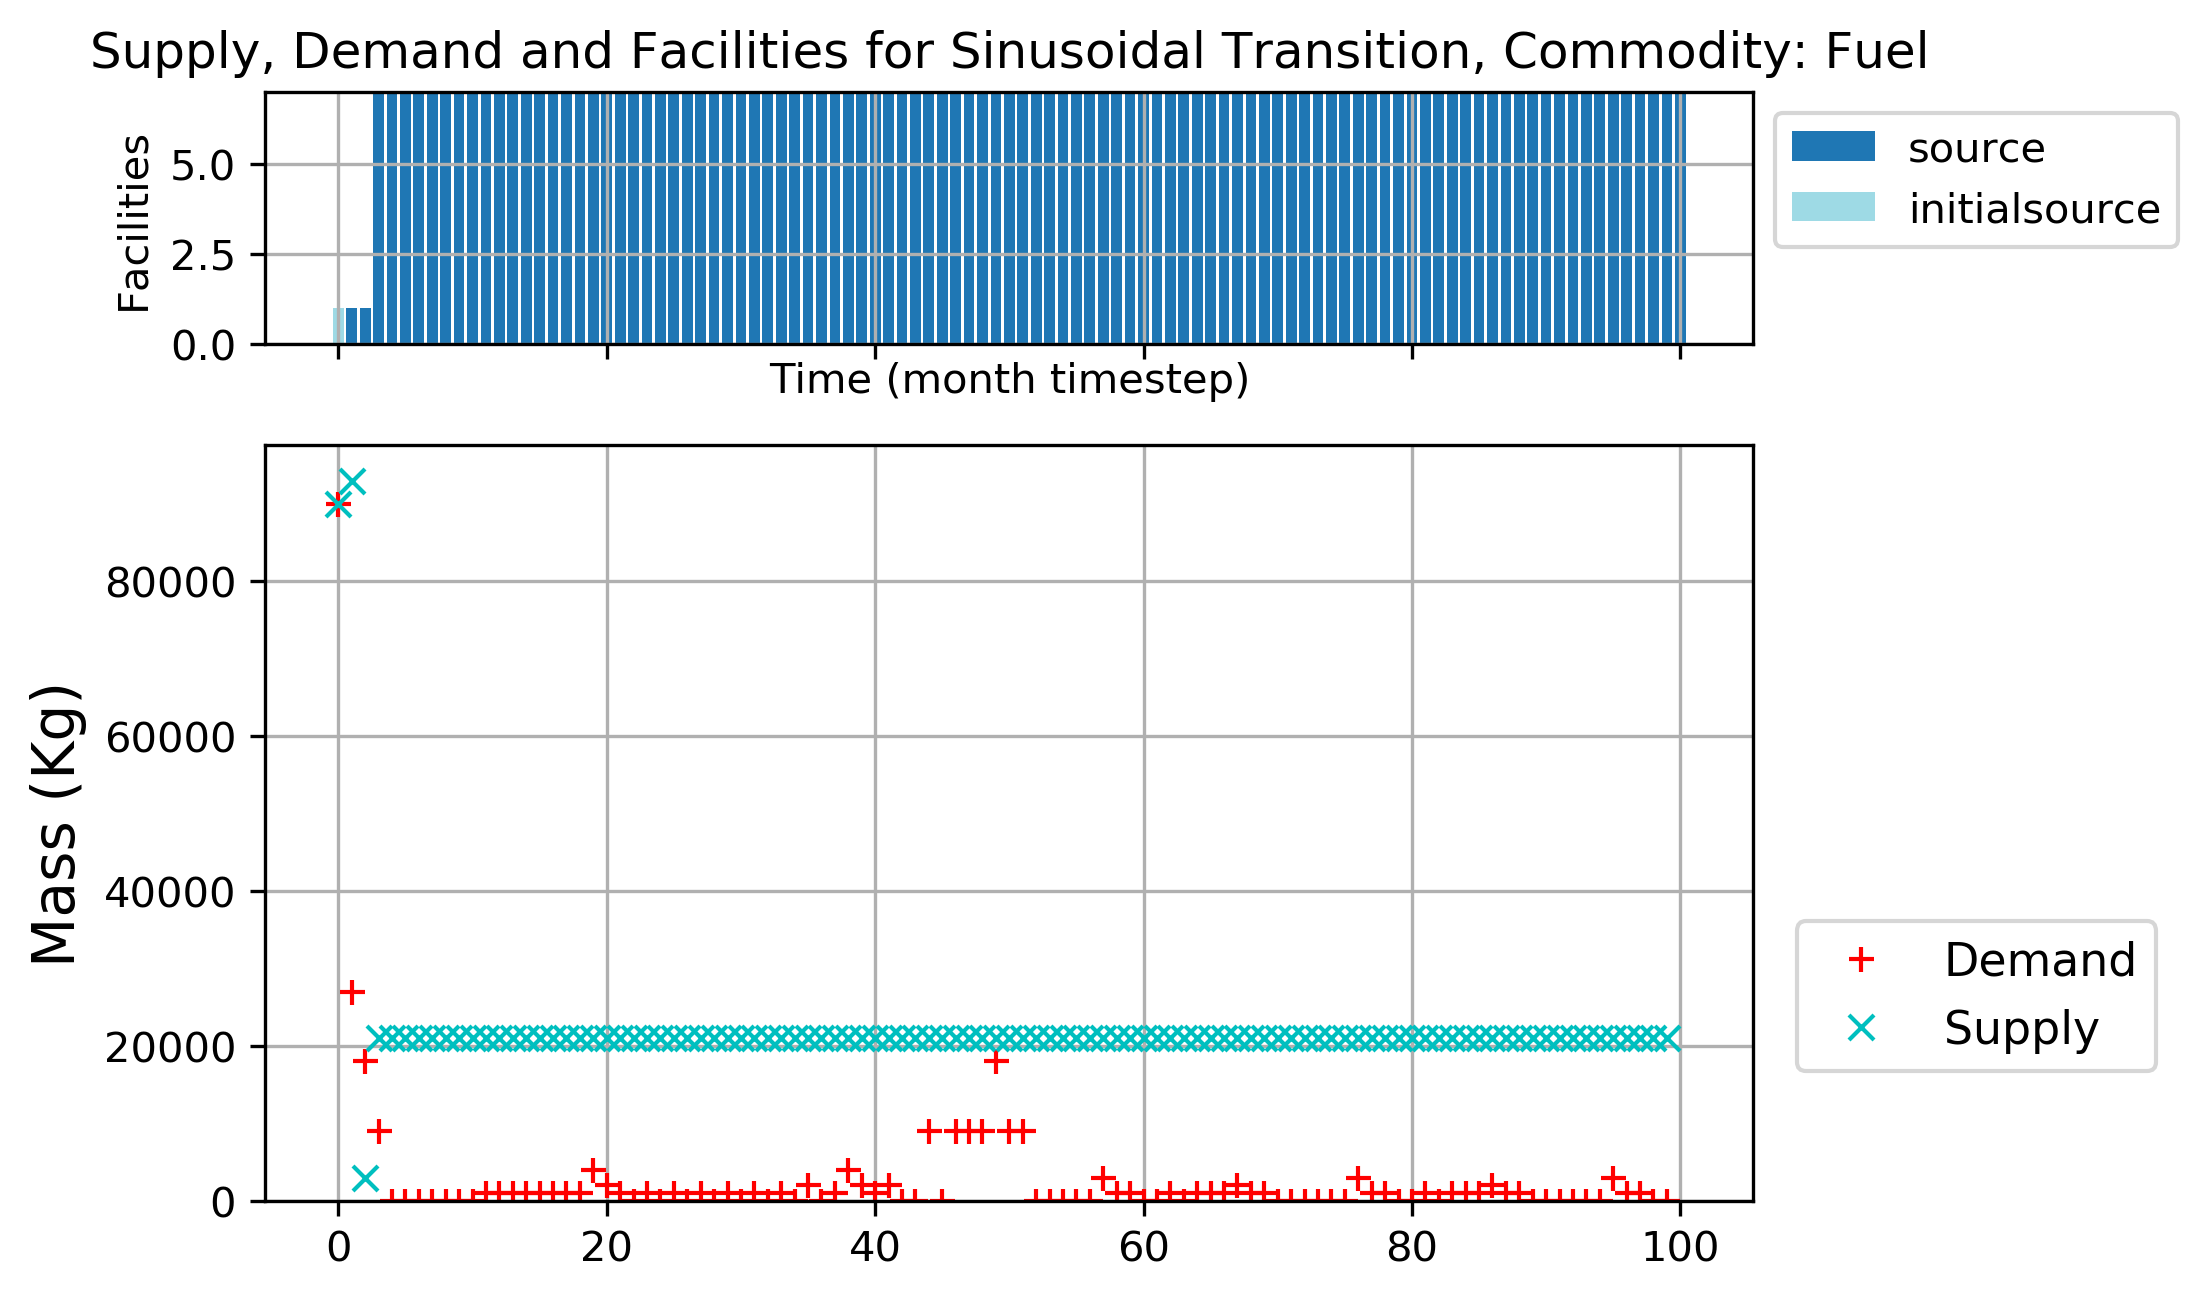
\includegraphics[width=\linewidth]{figures/sinetransition-fuel.png} 
        \caption{Fuel is demanded by reactors and supplied by source facilities.}
	    \label{fig:sinetransition-fuel}
    \end{subfigure}
    \begin{subfigure}[t]{0.65\textwidth}
        \centering
        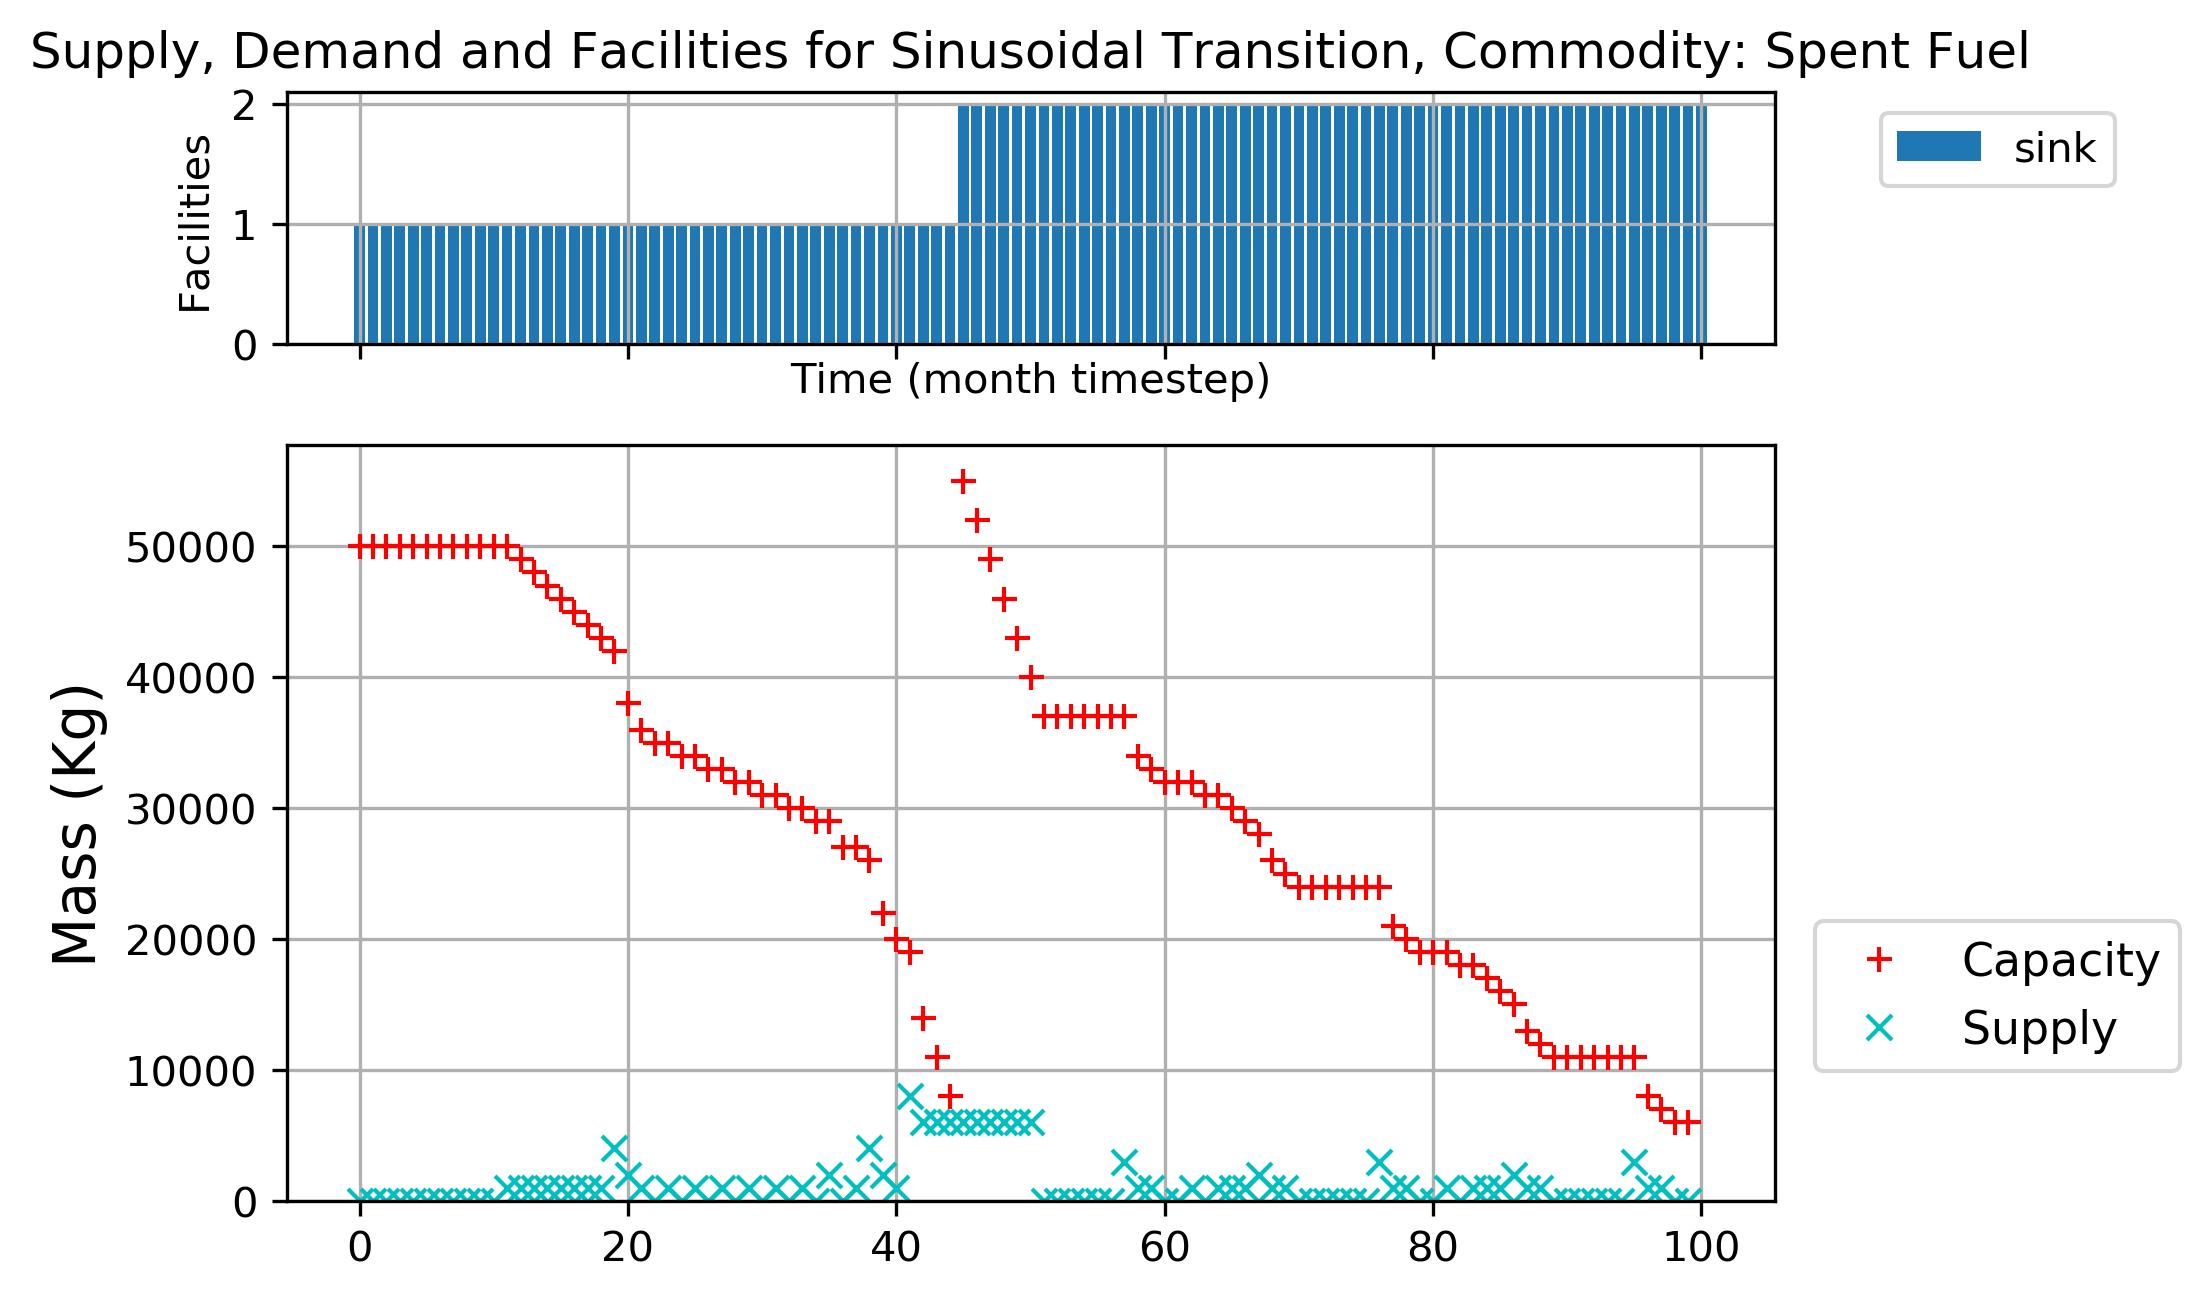
\includegraphics[width=\linewidth]{figures/sinetransition-spentfuel.png} 
        \caption{Spent Fuel is supplied by reactors and the capacity is provided by sink facilities.}
        \label{fig:sinetransition-spentfuel}
    \end{subfigure}
    \caption{Transition Scenario: Sinusoidal Power Demand}
\end{figure*}

\pagebreak
\section{Transition Scenarios}

The objective of this section was to carry out various simulations to validate 
\texttt{D3ploy}'s current capabilities for simulating complex cycles.
The Idaho National Laboratory Nuclear Fuel Cycle Evaluation and Screening Report \cite{wigeland_nuclear_2014} established several fuel cycle scenarios.
As part of the project NEUP-FY16-10512, the simulations focused on the cases EG01, EG23, EG24. The scenarios started at EG01 -- representing the current U.S. fuel cycle -- and transitioned to advanced fuel cycles.
The simulations utilized \texttt{d3ploy}'s NO, DO, and SO algorithms.

All the analyzed scenarios started at EG01. In EG01 all reactors were LWRs running a  once-through cycle burning enriched-U.
In EG23 fast reactors (FRs) produced all the power, relying on the continuous recycle of U/Pu supplemented by the addition of new natural-U to the cycle.
EG24 was similar to EG23, but its cycle utilized continuous recycling of U/TRU with the addition of new natural-U.

The present work focused on two transition scenarios: EG01-EG23 and EG01-EG24,  as shown in Figure \ref{fig:flow1}. The simulations started with a fleet of LWRs. After 80 years, the simulation progressively decommissioned the LWRs while transitioning to FRs. By the end of the cycle, all power was produced by FRs. Initial fueling of the FRs relied on reprocessed Pu from the LWR fleet. Following the transition, the FRs were able to produce their own Pu to sustain the cycle.

\begin{figure*}[]
	\centering
	\begin{subfigure}[t]{\textwidth}
		\centering
		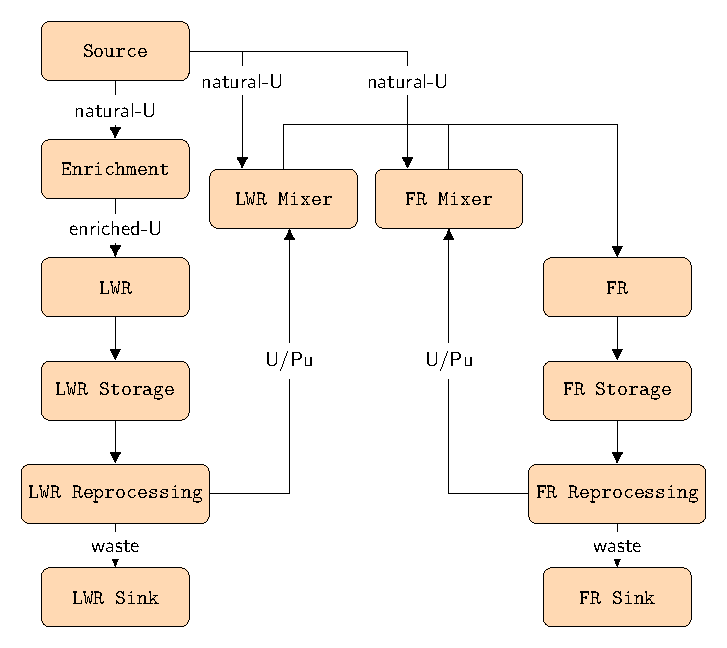
\includegraphics[width=0.7\linewidth]{23flow.pdf} 
		\caption{EG01-EG23.}
		\label{fig:23flow}
	\end{subfigure}
	\vspace{1cm}
	\begin{subfigure}[t]{\textwidth}
		\centering
		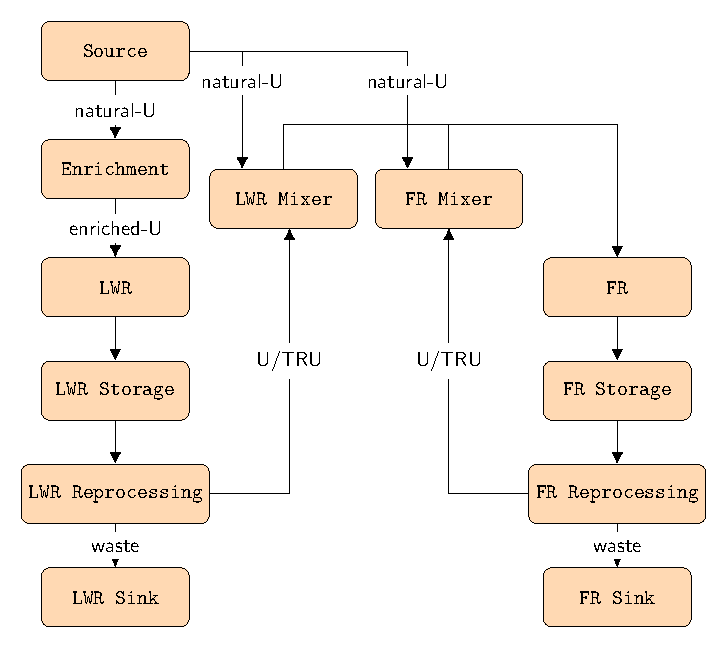
\includegraphics[width=0.7\linewidth]{24flow.pdf} 
		\caption{EG01-EG24.}
		\label{fig:24flow}
	\end{subfigure}
	\hfill
	\caption{Diagrams with facilities and mass flow of the scenarios EG01-EG23 and EG01-EG24.}
	\label{fig:flow1}
\end{figure*}

The following section presents the results for EG01-EG23 and EG01-EG24. The power demand was set at a constant 60 GW at all times. The transition scenarios used the capability of deploying facilities based on the difference between predicted demand and predicted supply, using a power supply buffer of 2000 MW. 

This section also includes a sensitivity analysis of the buffer size. A separate sensitivity analysis shows the dependency of the undersupply on the number of look-ahead time steps used to calculate the predicted demand and supply.

\subsection{EG01-EG23}

Figure \ref{fig:23power} shows the power demand and supply obtained using different prediction methods. Following it, Table \ref{tab:23-power} displays a comparison of the different algorithms. Table \ref{tab:23-power} presents the Cumulative Undersupply and the Cumulative Oversupply magnitudes. These values represent the summation of the difference between the power supplied and the power demanded for all the time steps in the simulation. This magnitude could best be thought of as energy. For undersupply conditions, the magnitude represents lack of energy provided during the time steps in which the supply did not meet the demand. Likewise, the oversupply would be the magnitude of excess energy produced.

\begin{table}[!h]
	\centering
	\caption{Undersupply and oversupply of Power for the different algorithms used to calculate EG01-EG23.}
	\label{tab:23-power}
        \begin{tabularx}{\textwidth}{lRRR}
		\hline
                Algorithm & Undersupplied & Cumulative  & Cumulative \\
                          & Timesteps     & Undersupply [GW]  & Oversupply [GW] \\ \hline
		MA        & 20 	& 20.0  &  920.5   \\ 
		ARMA      & 18 	&  7.7  &  1036.5  \\ 
		ARCH      &  0 	&   0  	&  1320.1  \\ 
		POLY      &  1 	&  0.3 	&  1783.5  \\ 
		EXP\_SMOOTHING 	& 20 	& 11.0 & 1473.5 \\ 
		HOLT-WINTERS  	& 20 	& 11.0 & 1473.5 \\ 
		FFT       & 2	& 60.3 	& 1751.9 	\\ 
		SW\_SEASONAL    & 20 	& 18.6 	& 1119.9 	\\ \hline
	\end{tabularx}
\end{table}

\begin{table}[!h]
	\centering
	\caption{Number of time steps with undersupply and under capacity of various commodities for the different algorithms used to calculate EG01-EG23.}
	\label{tab:23-commod}
        \begin{tabularx}{\textwidth}{l|RRR|RR}
		\hline
                & \multicolumn{3}{|c|}{Undersupply} & \multicolumn{2}{c}{Undercapacity} \\ \hline
		Algorithm & Natural U & Enriched U & FR fuel & LWR PU & FR PU \\ \hline
		MA        & 0 & 0 & 0 & 1 & 1 \\ 
		ARMA      & 0 & 0 & 0 & 1 & 1 \\ 
		ARCH      & 0 & 0 & 0 & 1 & 1 \\ 
		POLY      & 0 & 0 & 0 & 1 & 1 \\ 
		EXP\_SMOOTHING & 0 & 0 & 0 & 1 & 1 \\ 
		HOLT\_WINTERS  & 0 & 0 & 0 & 1 & 1 \\ 
		FFT       & 0 & 1 & 0 & 1 & 1 \\ 
		SW\_SEASONAL  & 0 & 0 & 0 & 1 & 1 \\ \hline
	\end{tabularx}
\end{table}

Table \ref{tab:23-commod} presents the number of time steps with undersupply of 
natural-U (sourceout), enriched-U (enrichmentout), and FR fuel. The table also 
displays the number of time steps in which the capacity of the LWR Mixer to process LWR Pu and the capacity of the FR Mixer to process FR Pu are not enough (undercapacity). In this table we notice that the supply of Pu and the deployment of the respective mixer has one time step of delay.

\begin{figure*}[!htbp]
	\centering
	\begin{subfigure}[t]{.95\textwidth}
		\centering
		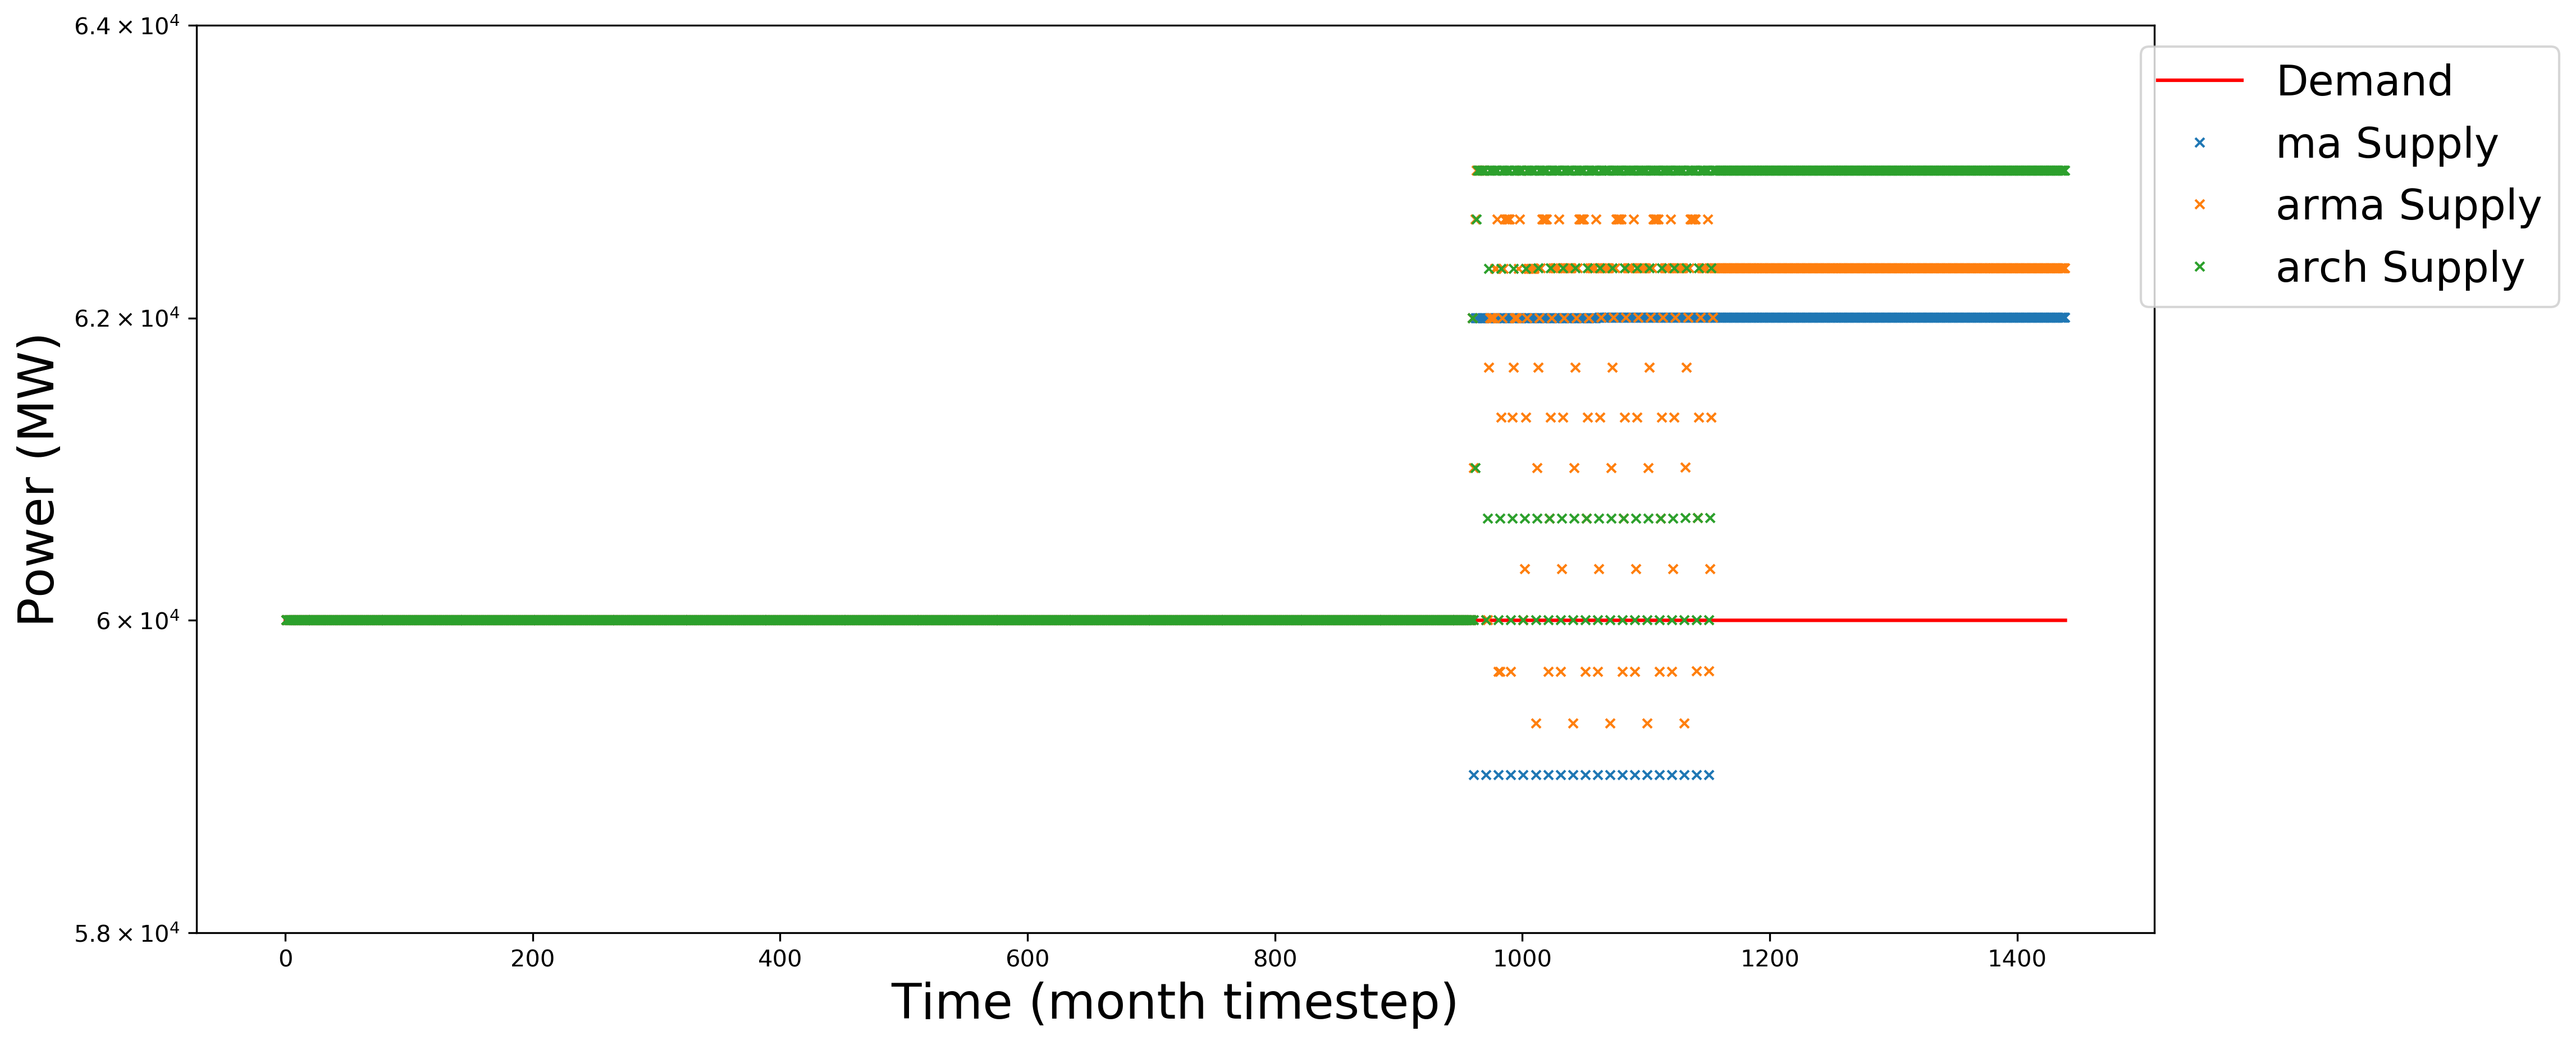
\includegraphics[width=\linewidth]{23-power-bufferB20001.png} 
		\caption{NO algorithms.}
		\label{fig:23powerNO}
	\end{subfigure}
	\vspace{.9cm}
	\begin{subfigure}[t]{.95\textwidth}
		\centering
		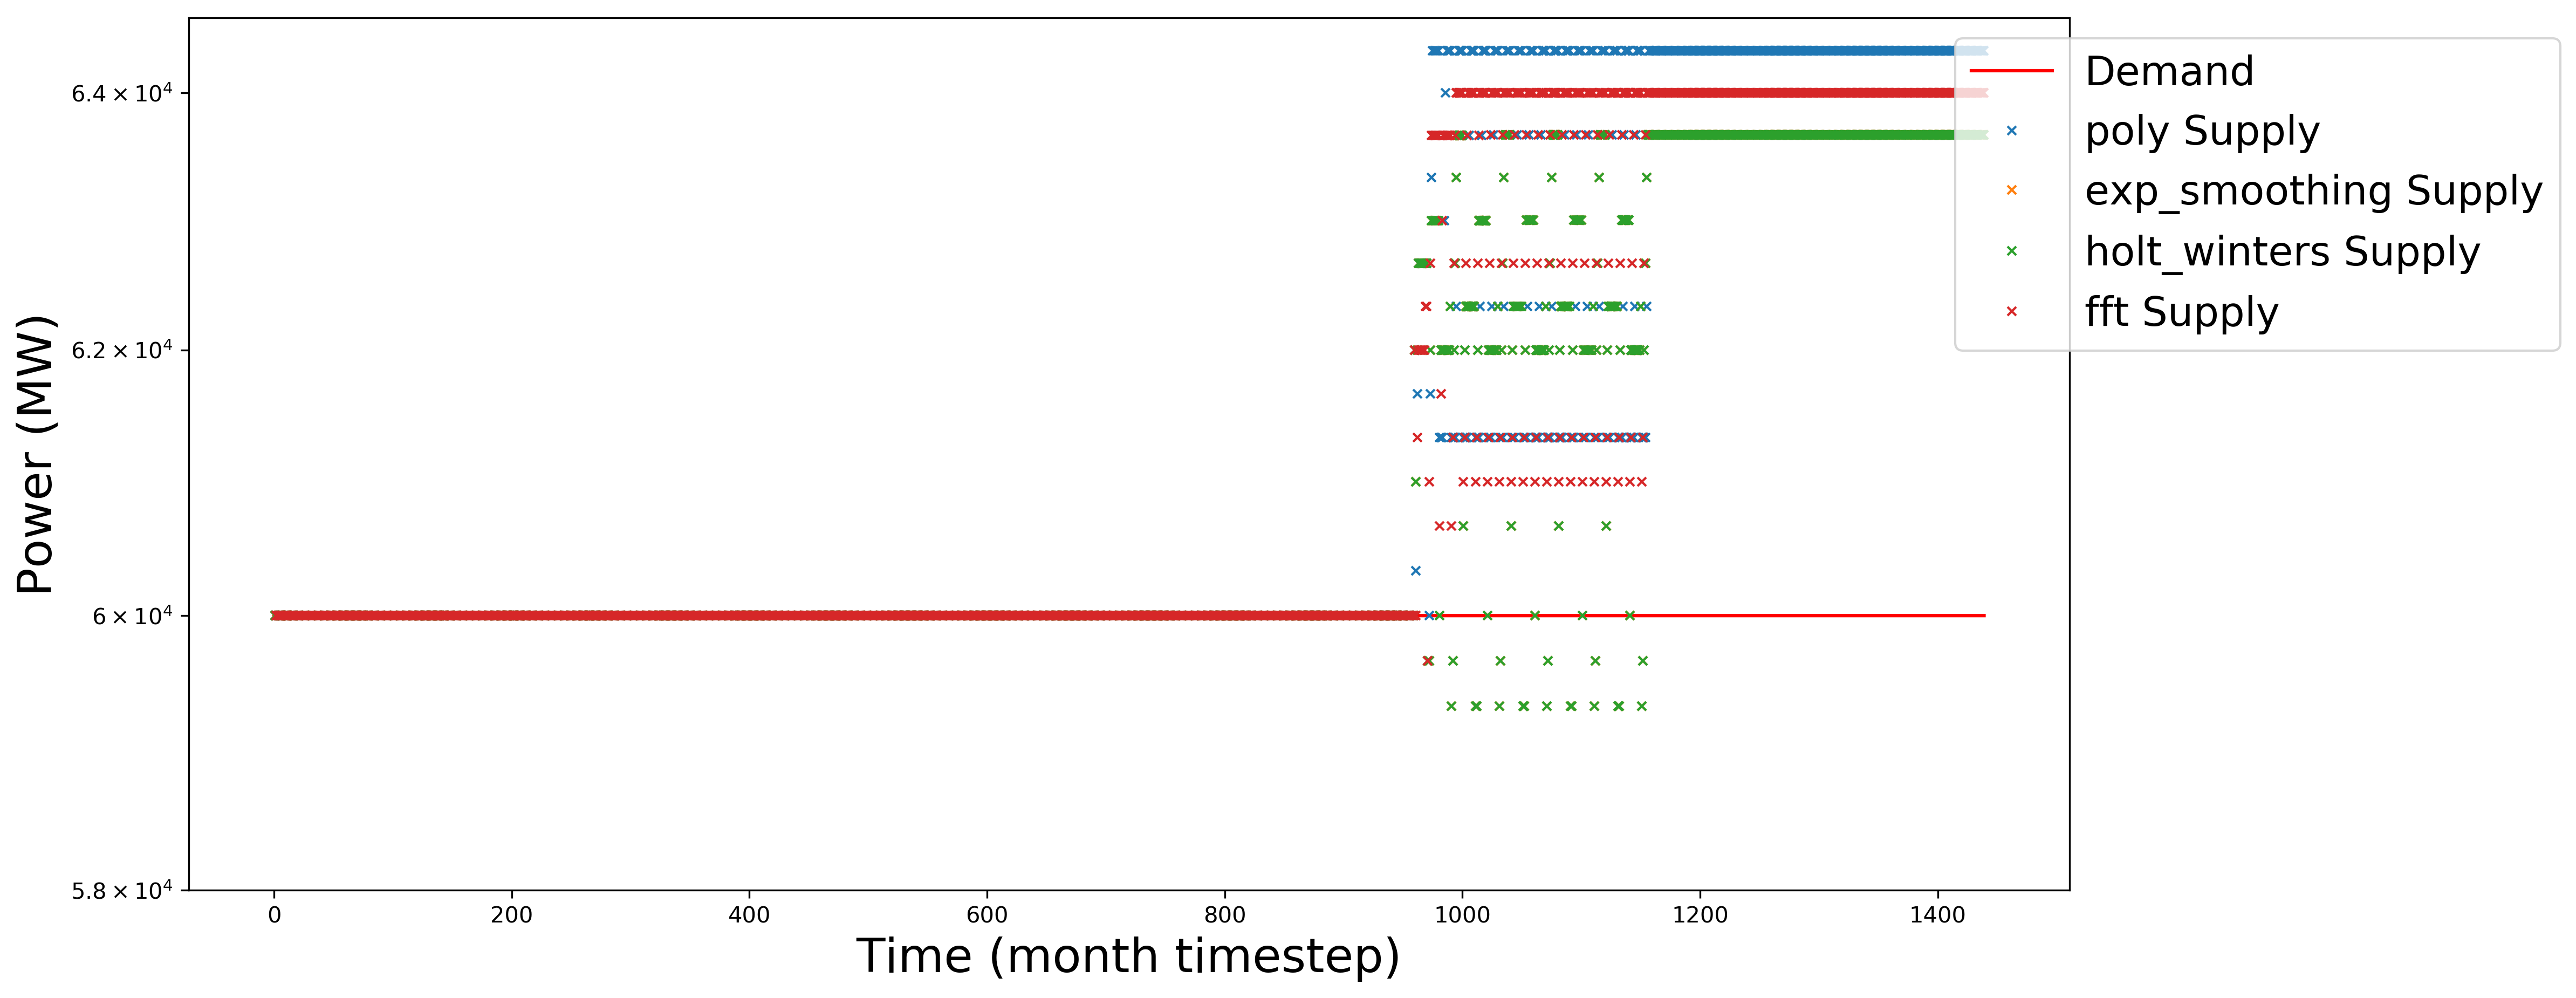
\includegraphics[width=\linewidth]{23-power-bufferB20002.png} 
		\caption{DO algorithms.}
		\label{fig:23powerDO}
	\end{subfigure}
	\vspace{.1cm}
	\begin{subfigure}[t]{.95\textwidth}
		\centering
		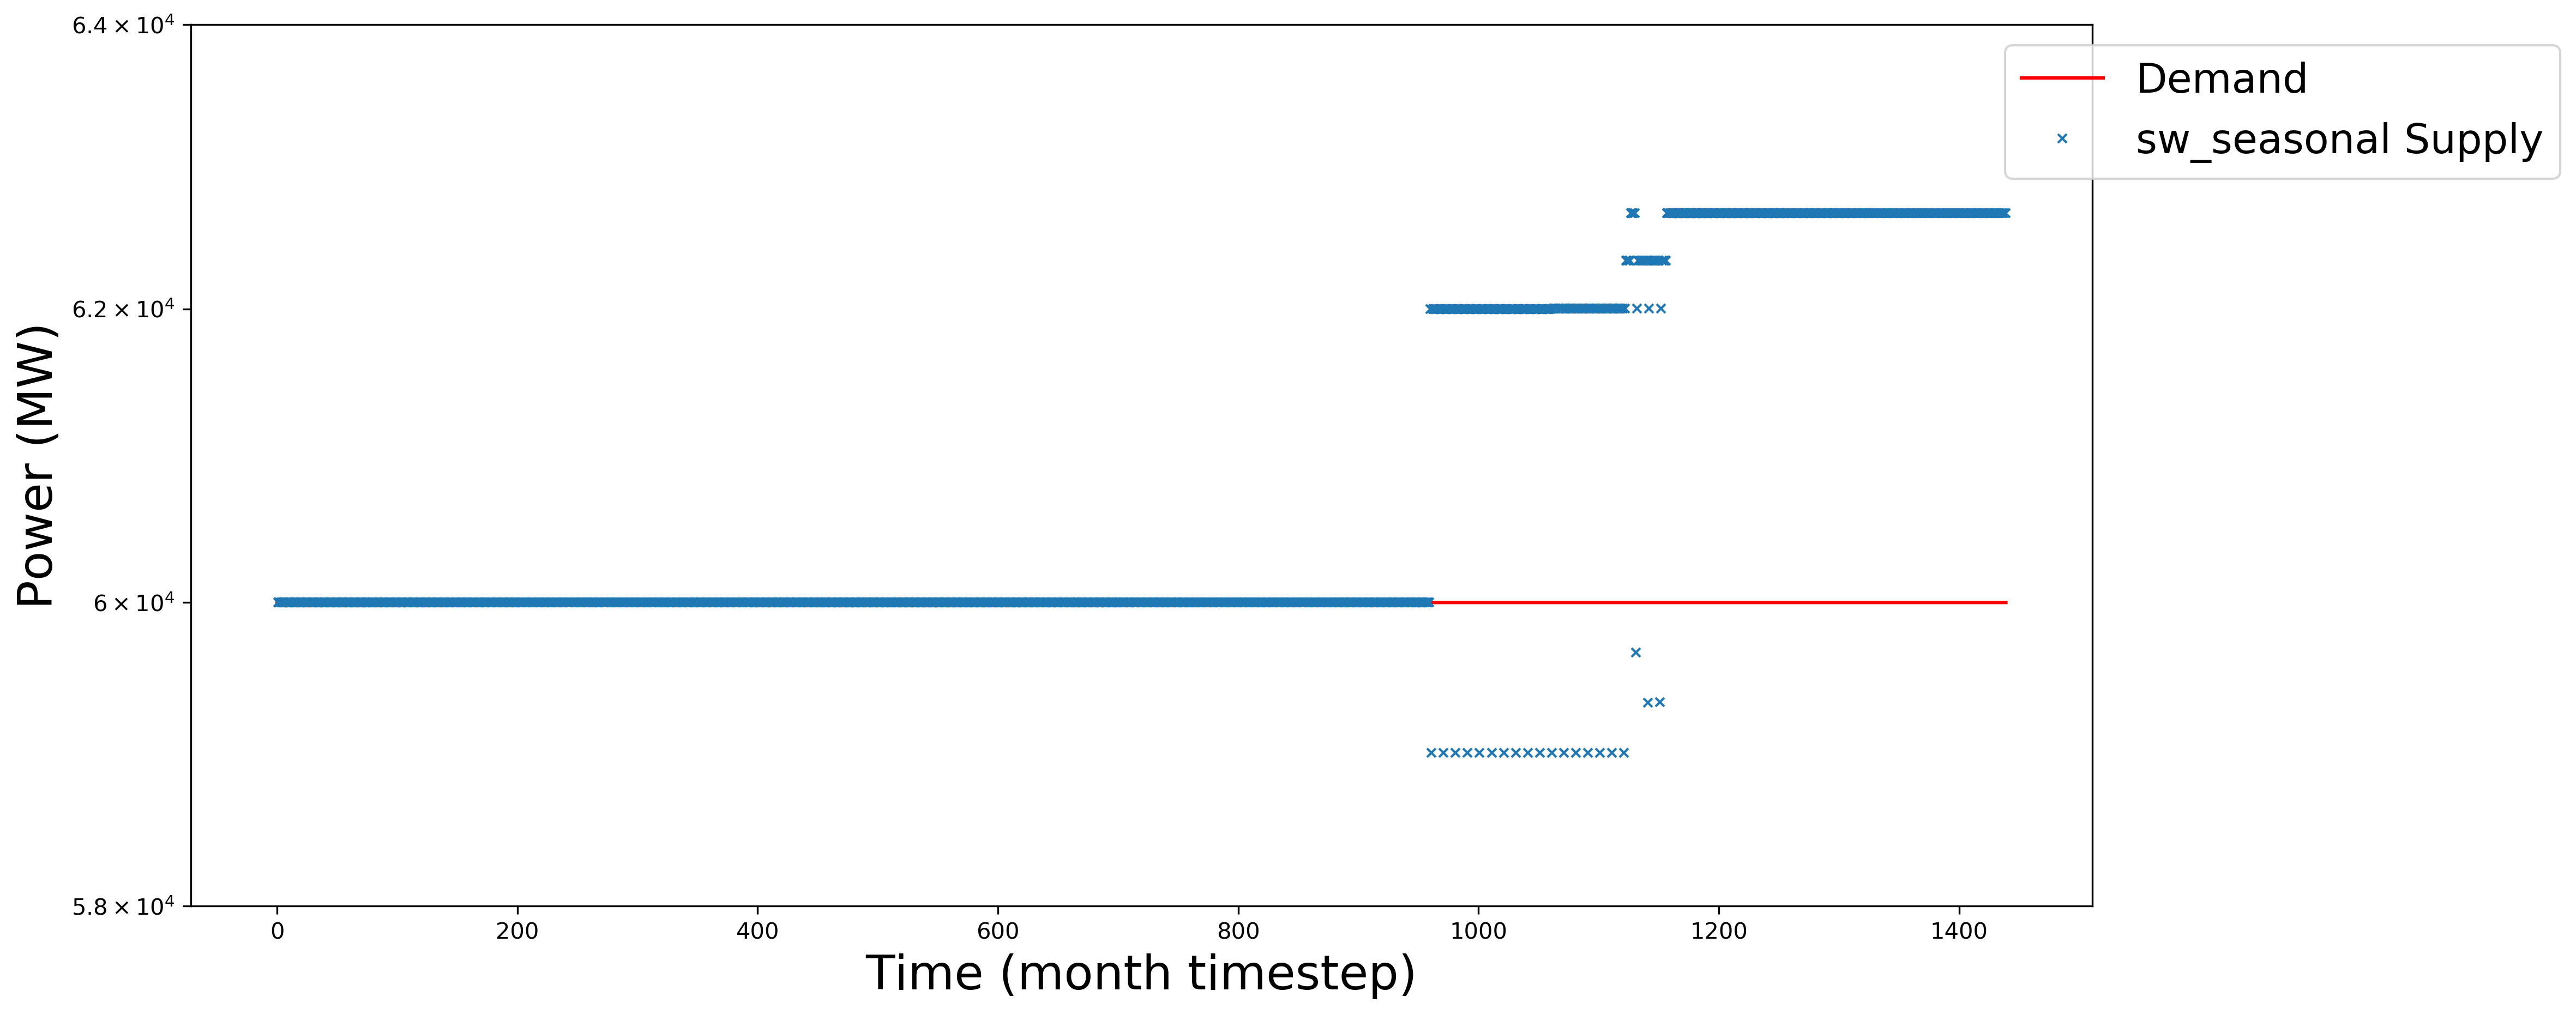
\includegraphics[width=\linewidth]{23-power-bufferB20003.png} 
		\caption{SO algorithms.}
		\label{fig:23powerSO}
	\end{subfigure}
	\hfill
	\caption{Plot of the power demand and supply of EG01-EG23 for a constant power demand of 60GW for different prediction algorithms.}
	\label{fig:23power}
\end{figure*}

One of the methods that performs the better is ARCH. For this scenario and said method, Figure \ref{fig:23-arch-commod} presents some of the different supply and demand time series plots for various commodities.
Figure \ref{fig:23-arch-sourceout} presents the number of Source facilities deployed, and the resultant demand and supply of natural-U. For this case, the capacity of natural-U supply is higher than the demand. We notice that the demand in the beginning of the simulation is higher than in the end. The LWRs use enriched-U produced by the enrichment of natural-U, while the FRs require a smaller quantity of U for their fuel. Figure \ref{fig:23-arch-lwrpu} displays the number of LWR Mixers deployed, and the supply and the capacity of LWR Pu (Pu produced by the LWRs). Logically, the supply of Pu decreases as the LWRs stop operating. Figure \ref{fig:23-arch-frpu} shows the FR Mixers, and the supply and capacity of FR Pu. The supply of Pu increases as \deploy deploys new FRs.

\begin{figure*}[!htbp]
	\centering
	\begin{subfigure}[t]{.8\textwidth}
		\centering
		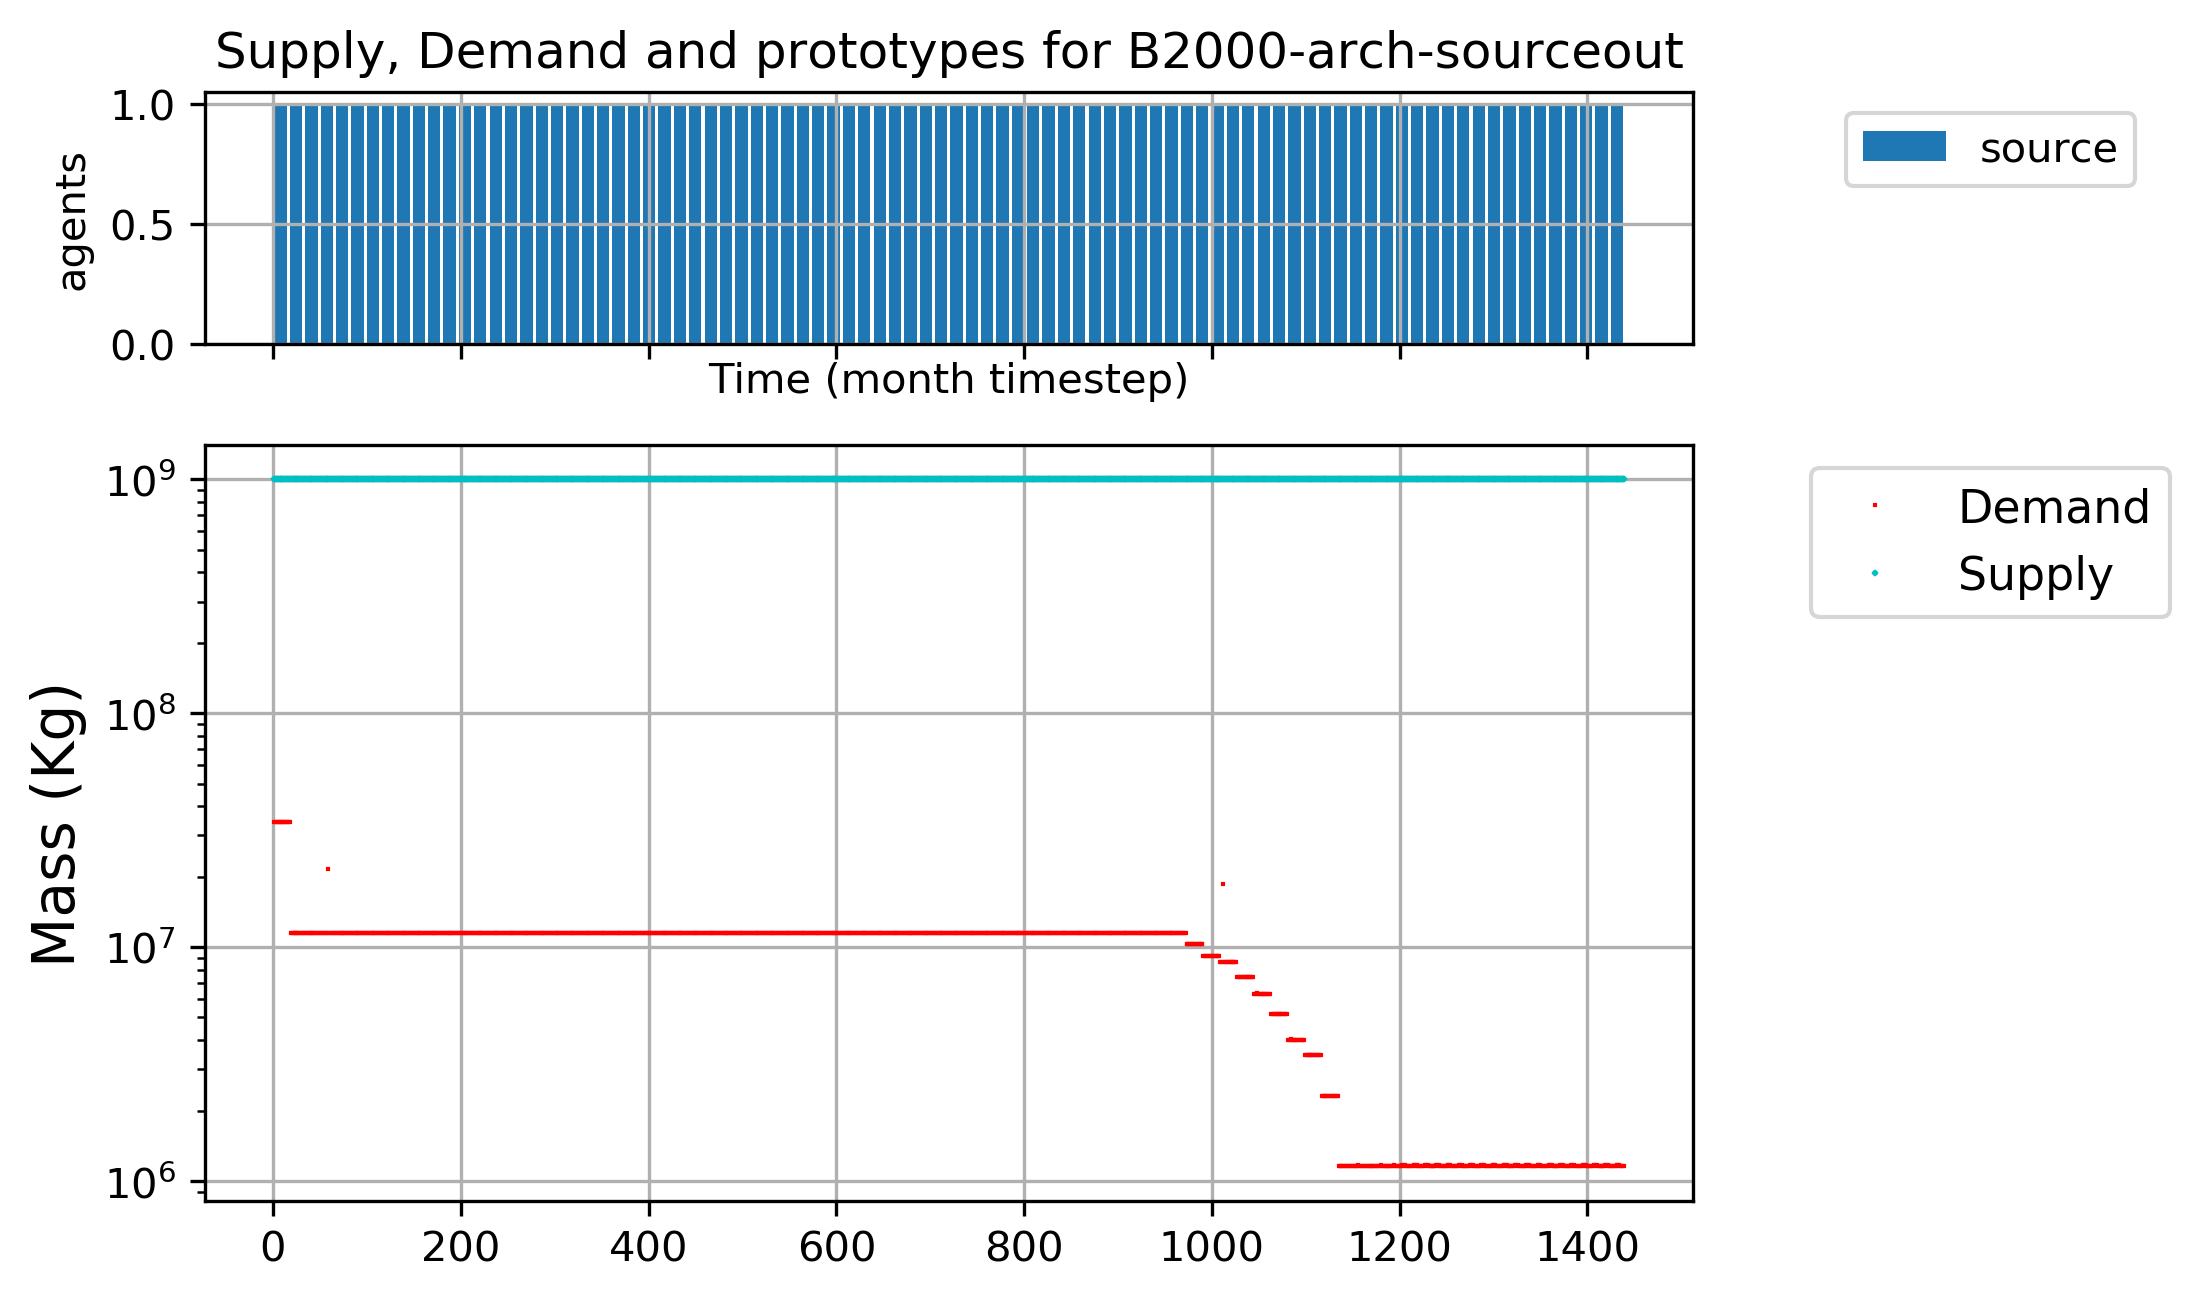
\includegraphics[width=\linewidth]{B2000-arch-sourceout.png} 
		\caption{Production of natural-U by the source.}
		\label{fig:23-arch-sourceout}
	\end{subfigure}
	\vspace{.9cm}
	\begin{subfigure}[t]{.45\textwidth}
		\centering
		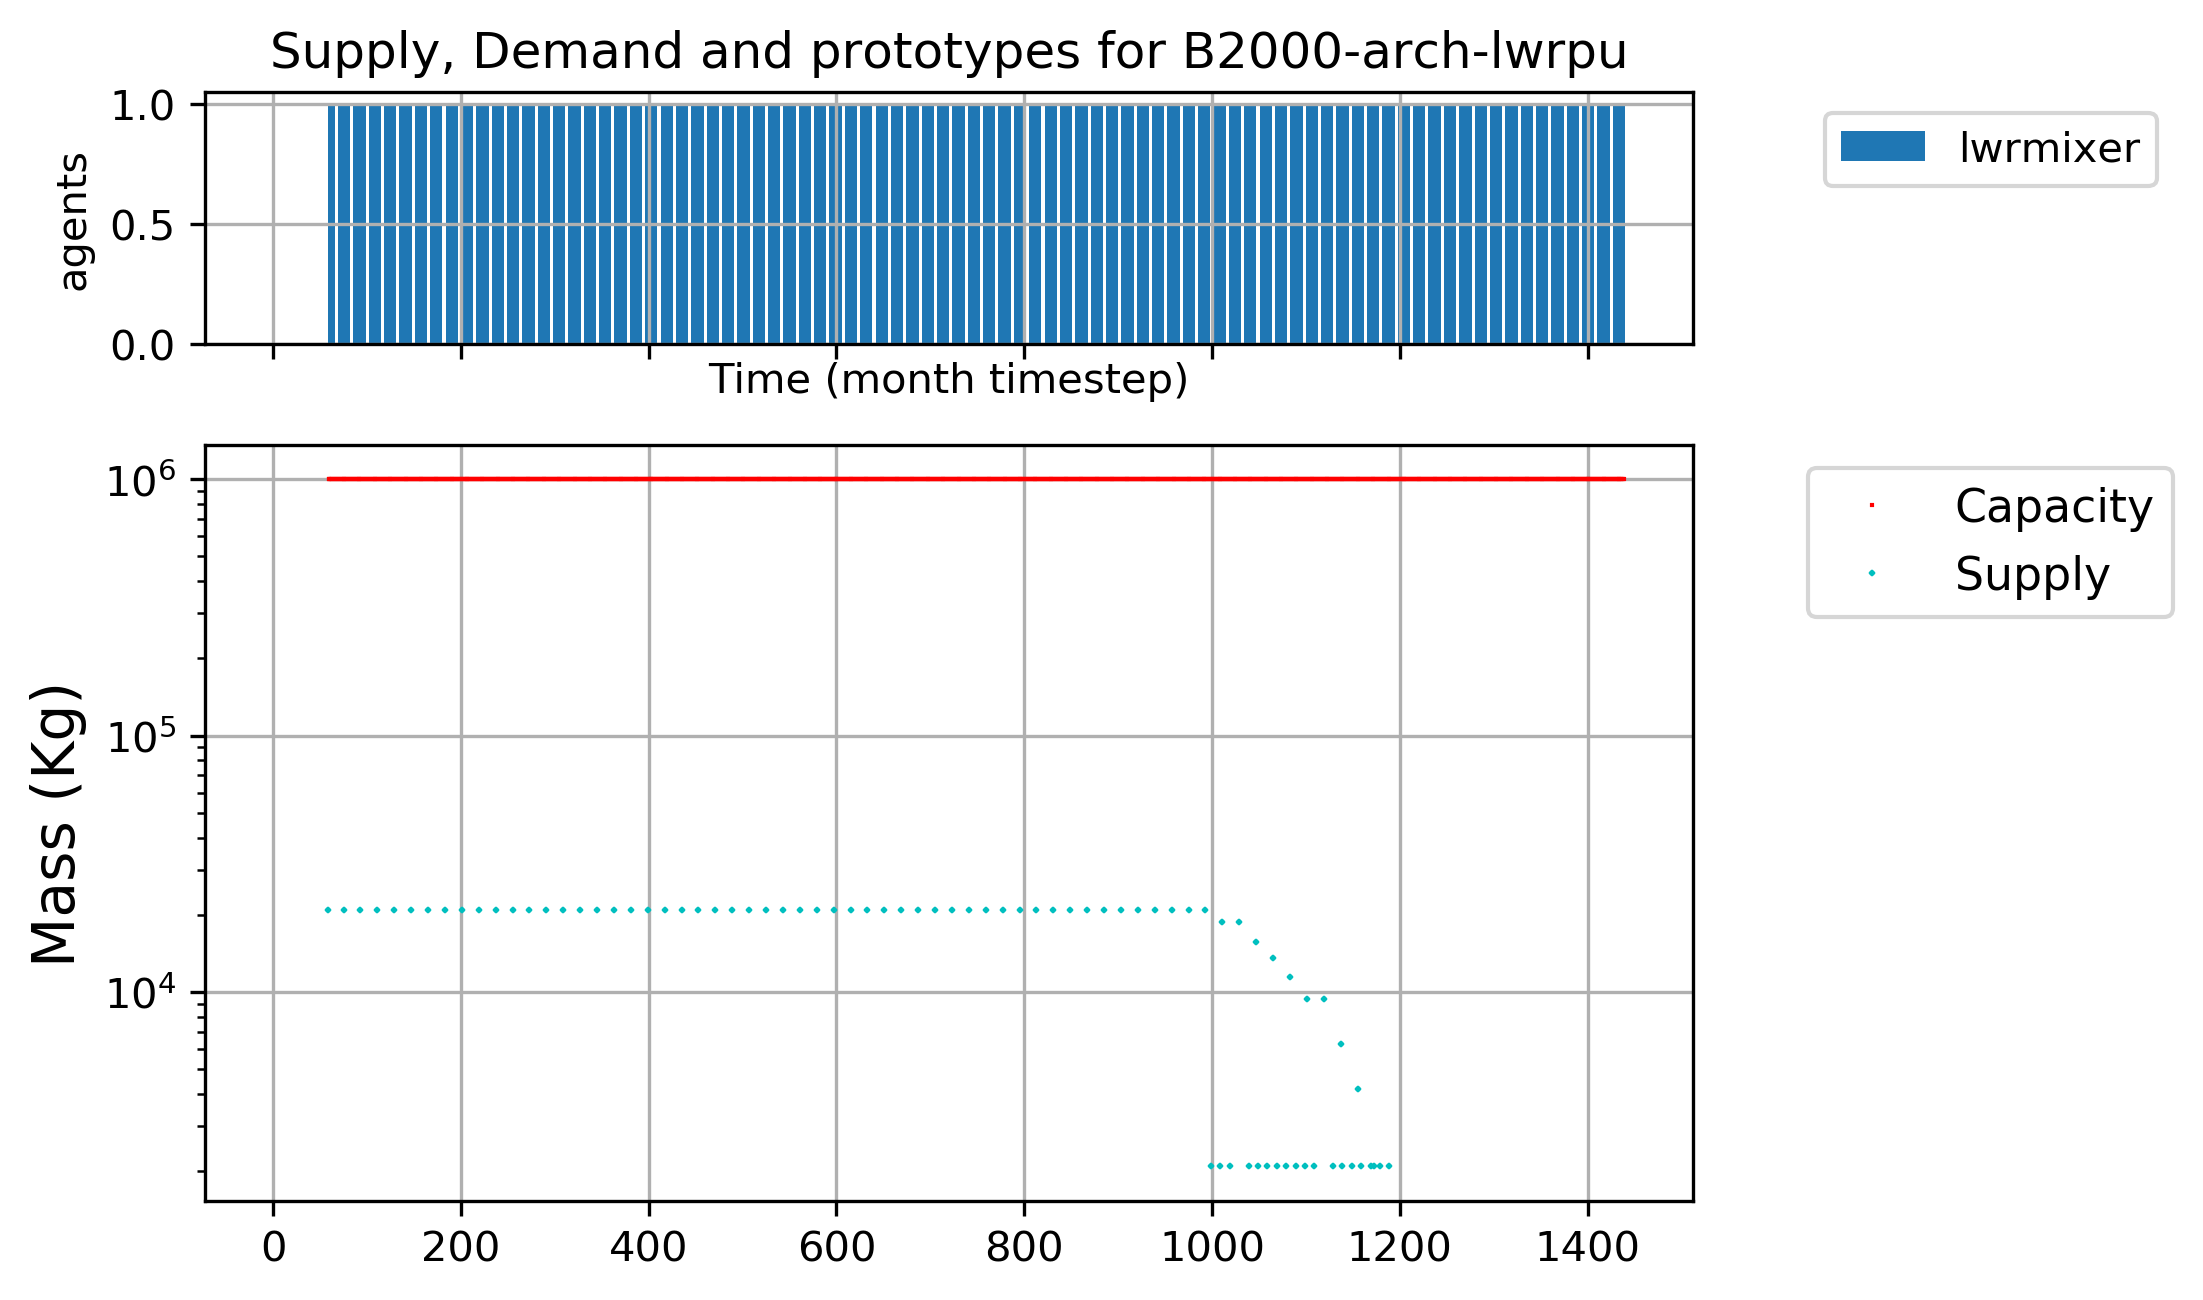
\includegraphics[width=\linewidth]{B2000-arch-lwrpu.png} 
		\caption{Pu produced by the LWRs and exchanged to the LWR Mixer.}
		\label{fig:23-arch-lwrpu}
	\end{subfigure}
	\begin{subfigure}[t]{.45\textwidth}
	\centering
	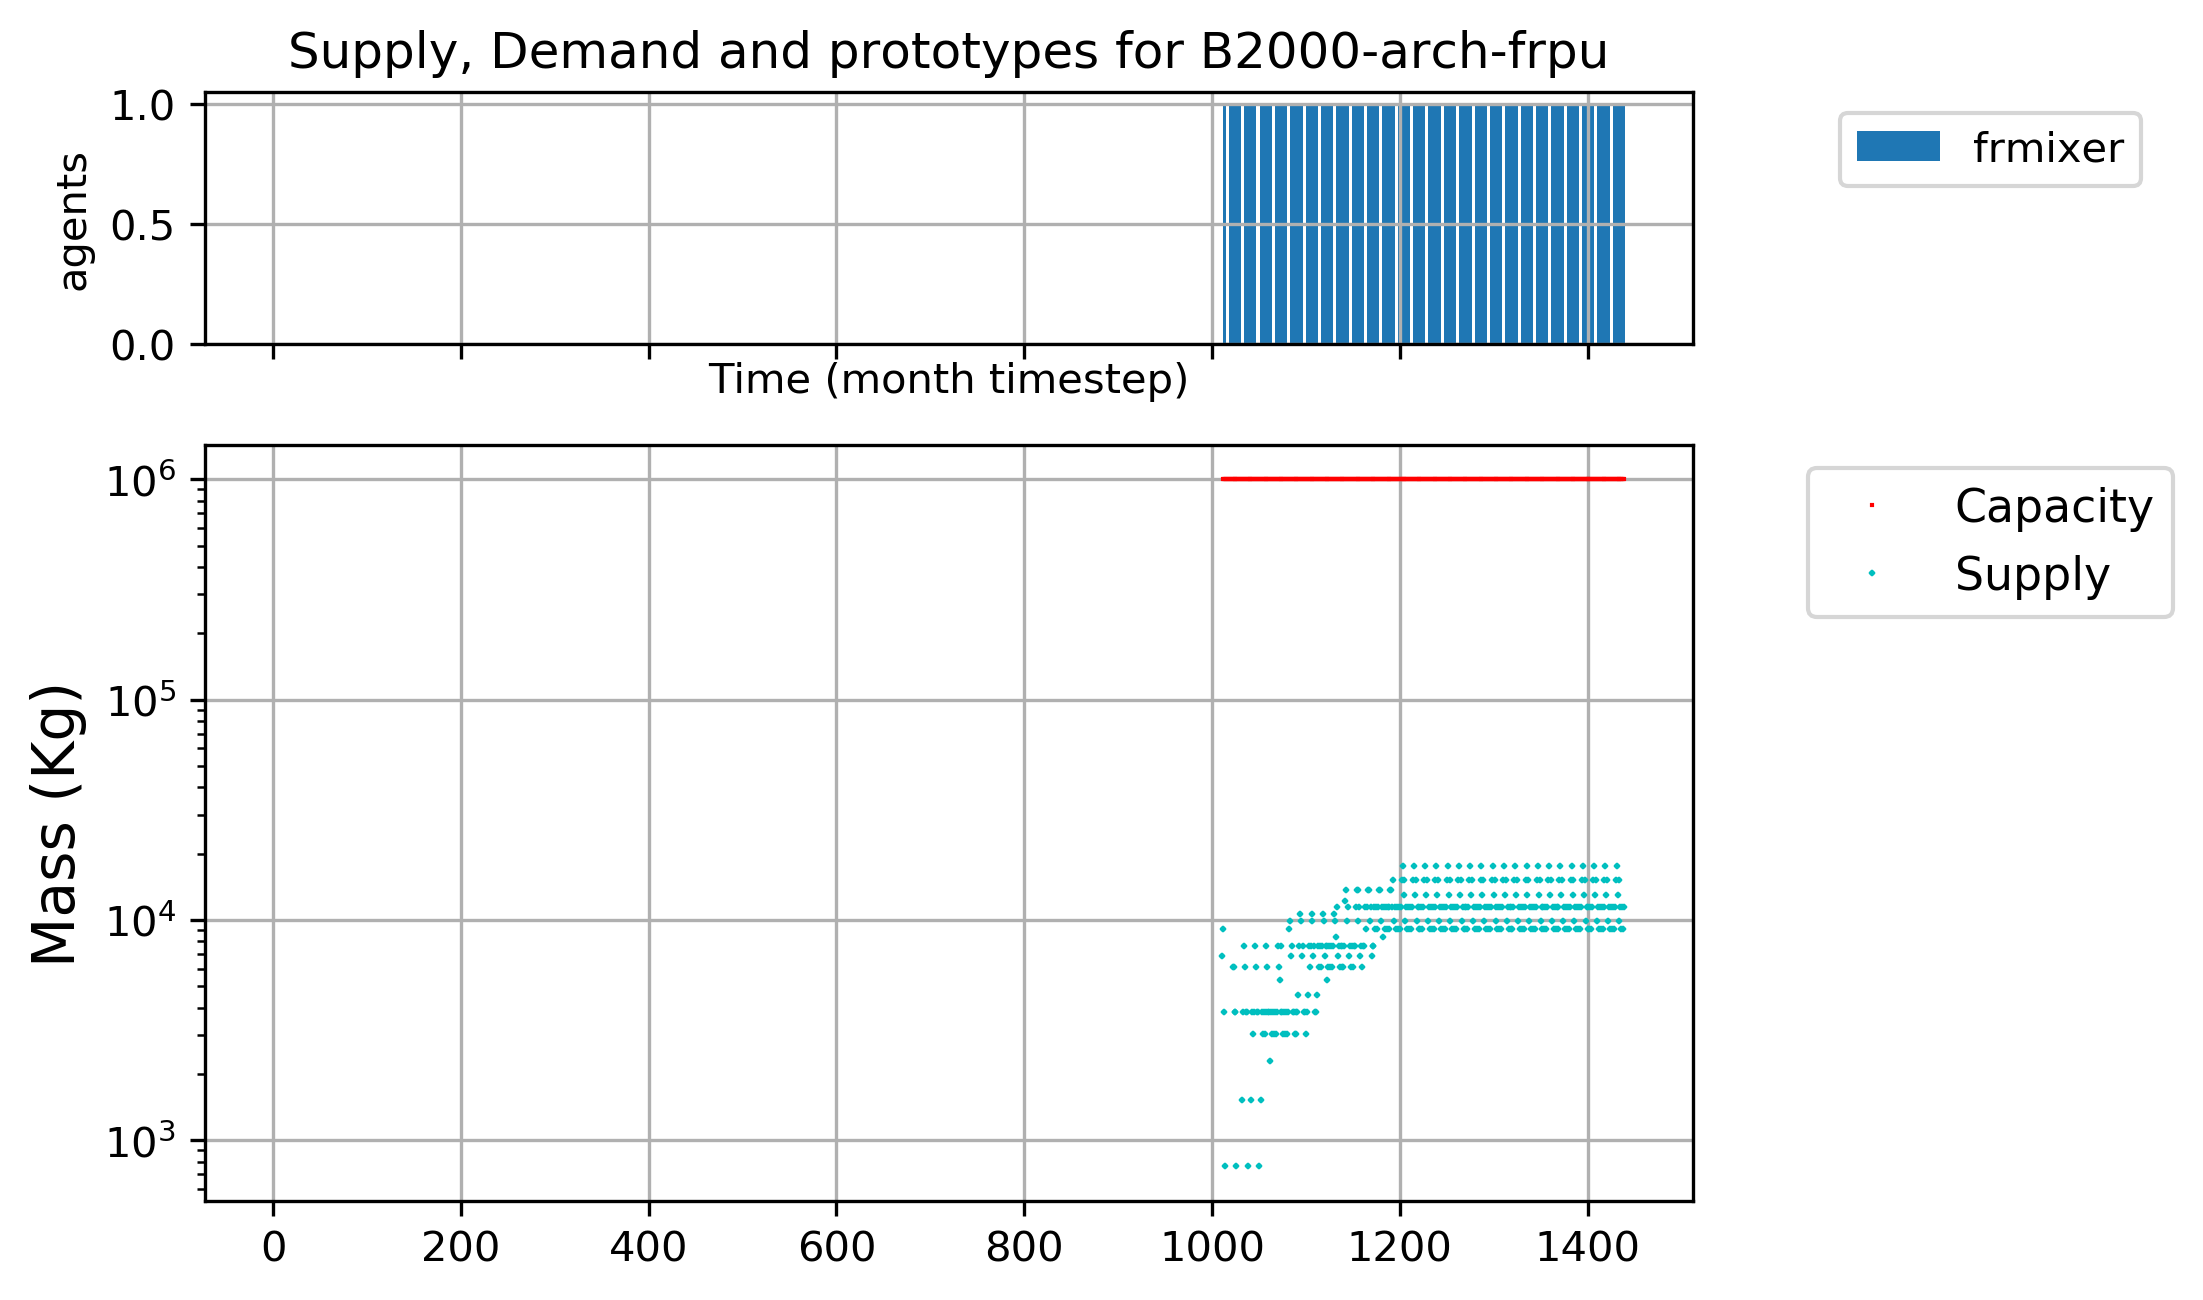
\includegraphics[width=\linewidth]{B2000-arch-frpu.png} 
	\caption{Pu produced by the FRs and exchanged to the FR Mixer.}
	\label{fig:23-arch-frpu}
\end{subfigure}
	\hfill
	\caption{Plot for different commodities EG01-EG23.}
	\label{fig:23-arch-commod}
\end{figure*}

\subsection{EG01-EG24}

Figure \ref{fig:24power} shows the power demand and supply obtained using different prediction methods. Following it, Tables \ref{tab:24-power} and \ref{tab:24-commod} display a comparison of the different algorithms.

\begin{table}[!h]
	\centering
        \caption{Undersupply and oversupply of power with the different 
        algorithms used to drive EG01-EG24.}
	\label{tab:24-power}
        \begin{tabularx}{\textwidth}{l|RRR}
		\hline
		& \multicolumn{3}{|c}{Power} \\ \hline
		Algorithm & Undersupplied Time Steps  & 
		Cumulative Undersupply [GW]  & Cumulative Oversupply [GW] \\ \hline
		MA        & 20.0 	& 20.0  &  920.5   \\ 
		ARMA      & 18.0 	&  7.7  &  1036.5  \\ 
		ARCH      &  0 	&   0  	&  1320.1  \\ 
		POLY      &  1.0 	&  0.3 	&  1783.5  \\ 
		EXP\_SMOOTHING 	& 20.0 	& 11.0 & 1473.5 \\ 
		HOLT-WINTERS  	& 20.0 	& 11.0 & 1473.5 \\ 
		FFT       & 2.0 	& 60.3 	& 1751.9\\ 
		SW\_SEASONAL    & 20.0 	& 18.6 	& 1119.9 \\ \hline
	\end{tabularx}
\end{table}

\begin{table}[!h]
	\centering
	\caption {Number of time steps with undersupply and under capacity of various commodities for the different algorithms used to calculate EG01-EG24.}
	\label{tab:24-commod}
        \begin{tabularx}{\textwidth}{l|RRR|RR}
		\hline
                & \multicolumn{3}{|c}{Undersupply} & \multicolumn{2}{|c}{Undercapacity} \\ \hline
		Algorithm & Natural U & Enriched U & FR fuel & LWR PU & FR PU \\ \hline
		MA        & 0 & 0 & 0 & 1 & 1 \\ 
		ARMA      & 0 & 0 & 0 & 1 & 1 \\ 
		ARCH      & 0 & 0 & 0 & 1 & 1 \\ 
		POLY      & 0 & 0 & 0 & 1 & 1 \\ 
		EXP\_SMOOTHING & 0 & 0 & 0 & 1 & 1 \\ 
		HOLT\_WINTERS  & 0 & 0 & 0 & 1 & 1 \\ 
		FFT       & 0 & 1 & 0 & 1 & 1 \\ 
		SW\_SEASONAL  & 0 & 0 & 0 & 1 & 1 \\ \hline
	\end{tabularx}
\end{table}

\begin{figure*}[!htbp]
	\centering
	\begin{subfigure}[t]{\textwidth}
		\centering
		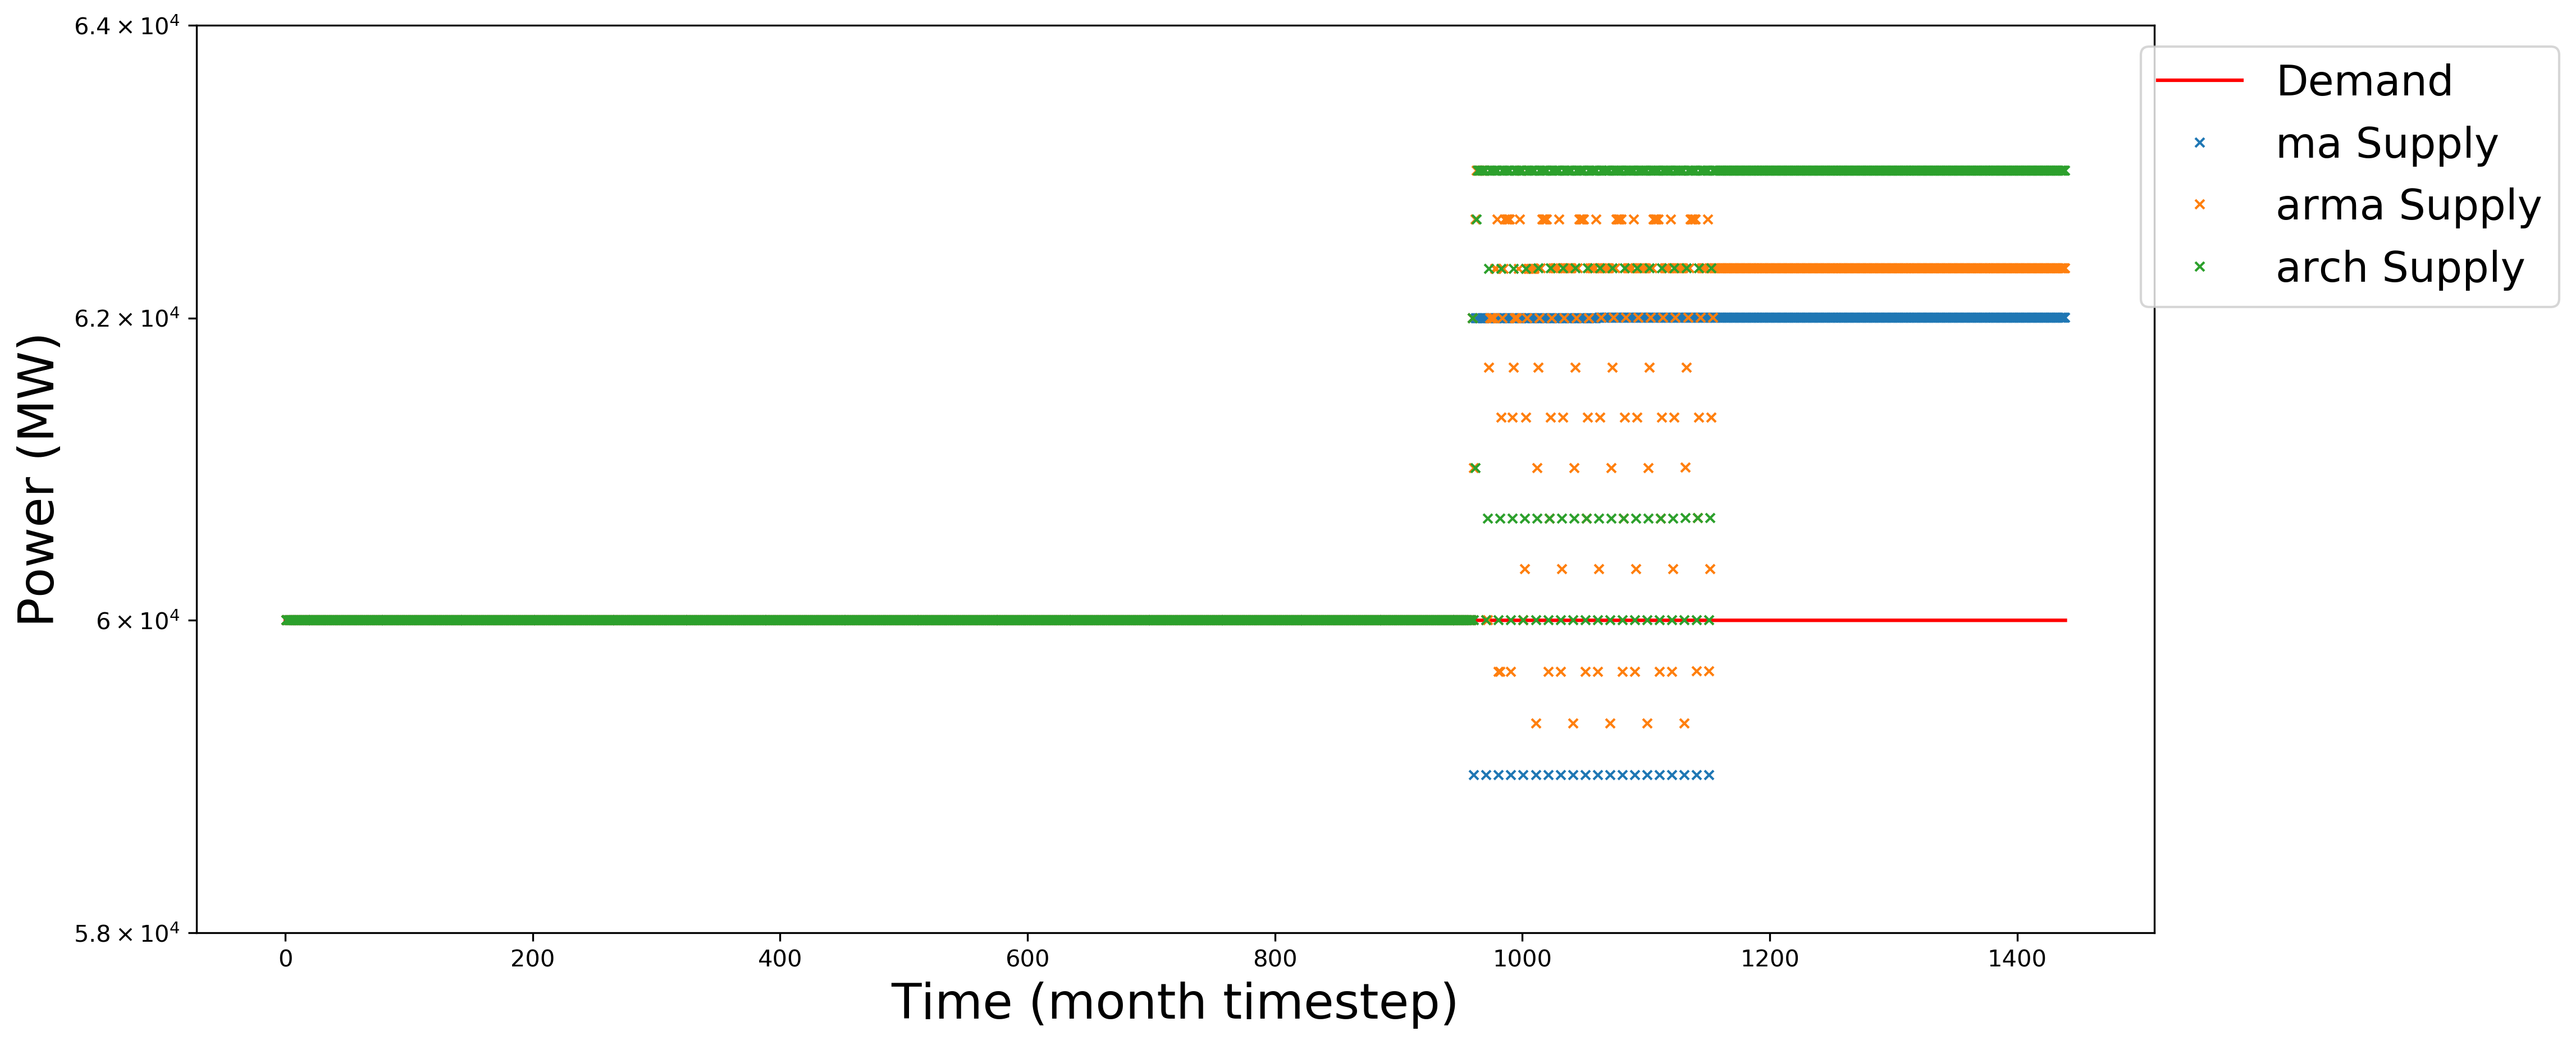
\includegraphics[width=\linewidth]{24-power-bufferB20001.png} 
		\caption{NO algorithms.}
		\label{fig:24powerNO}
	\end{subfigure}
	\vspace{1cm}
	\begin{subfigure}[t]{\textwidth}
		\centering
		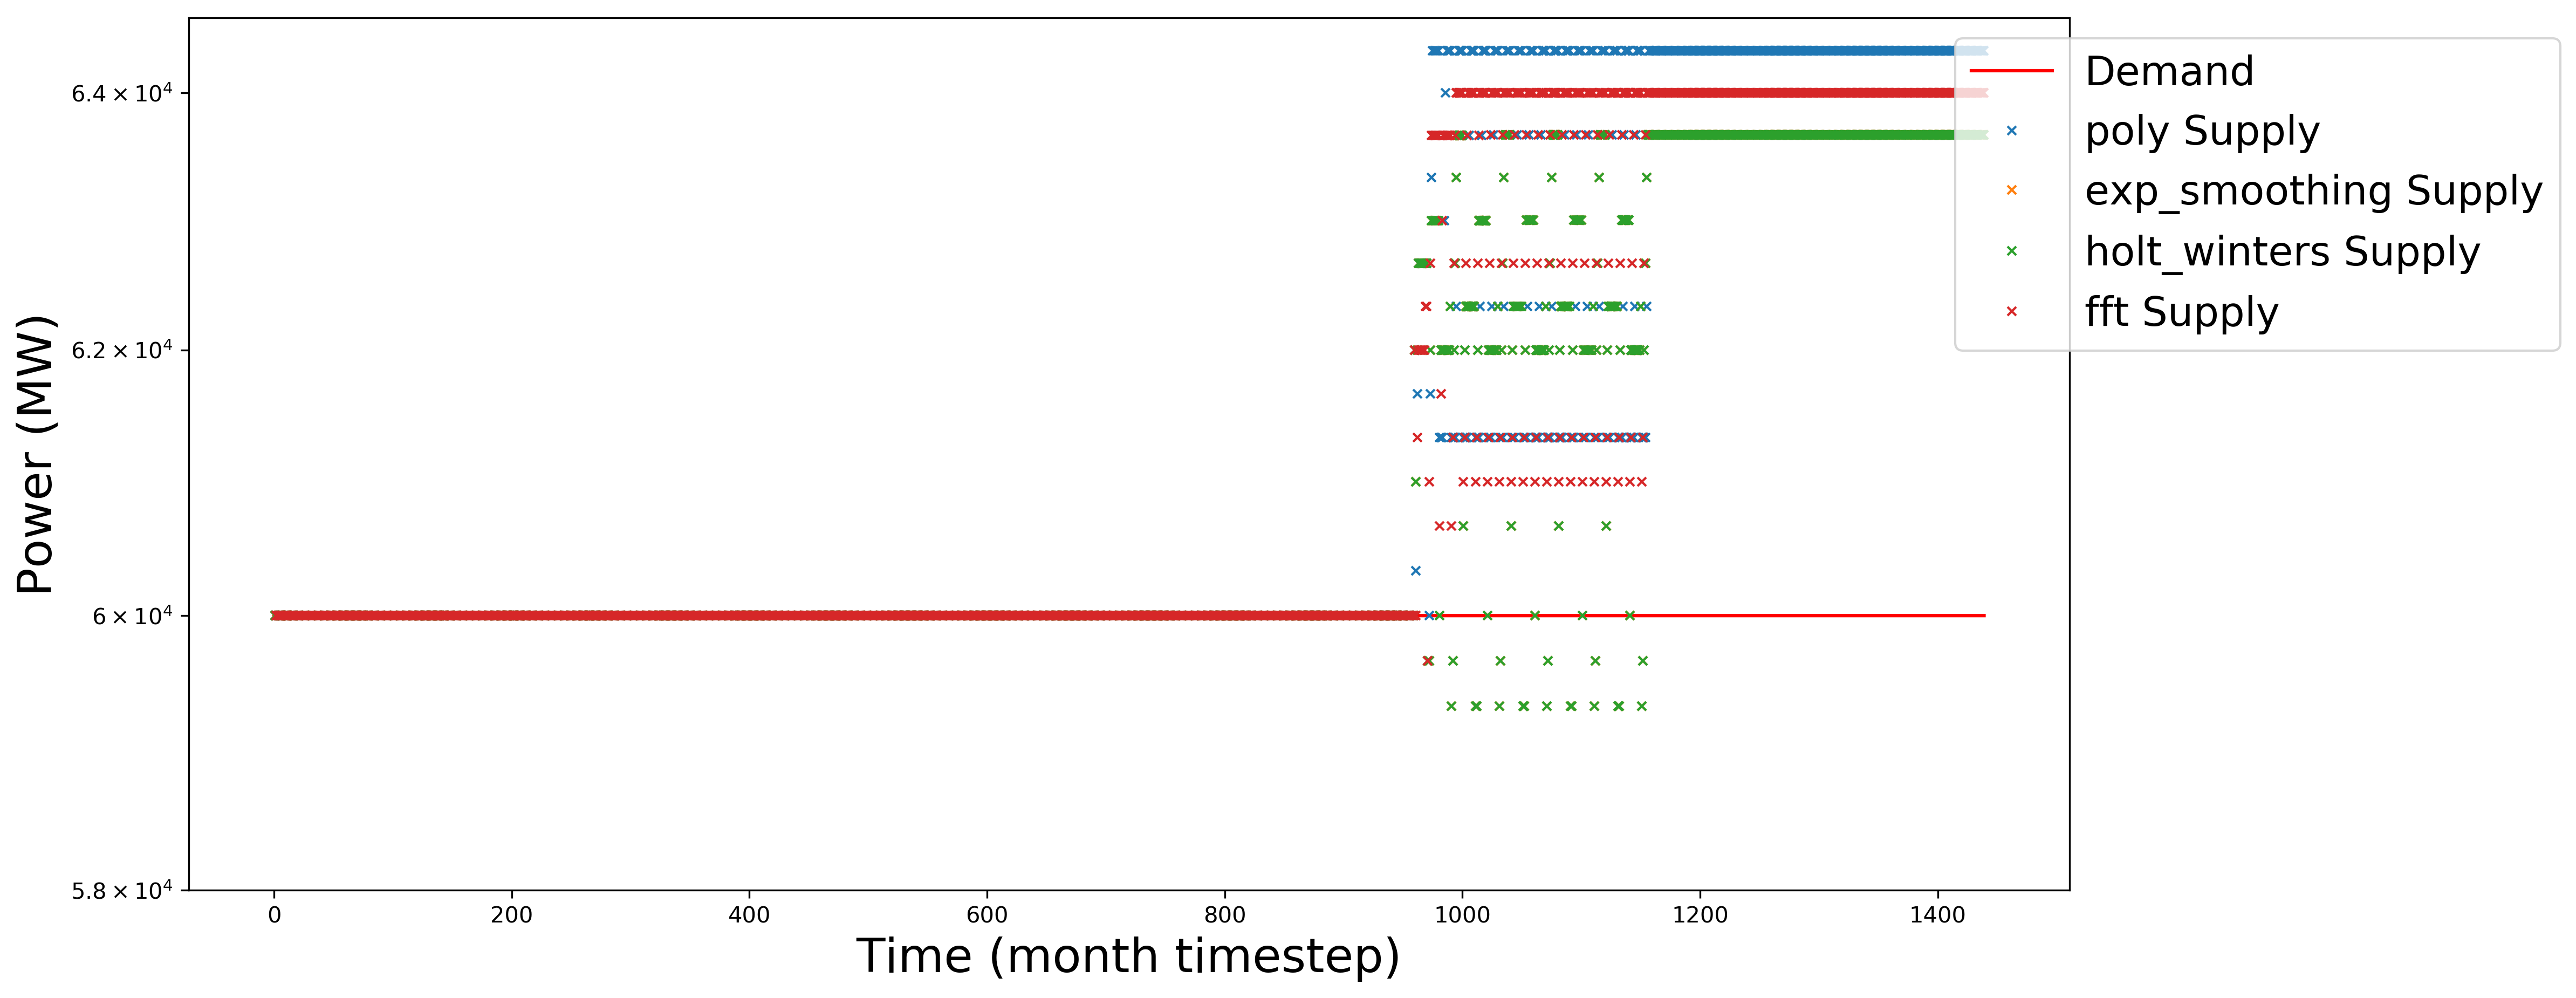
\includegraphics[width=\linewidth]{24-power-bufferB20002.png} 
		\caption{DO algorithms.}
		\label{fig:24powerDO}
	\end{subfigure}
	\begin{subfigure}[t]{.95\textwidth}
		\centering
		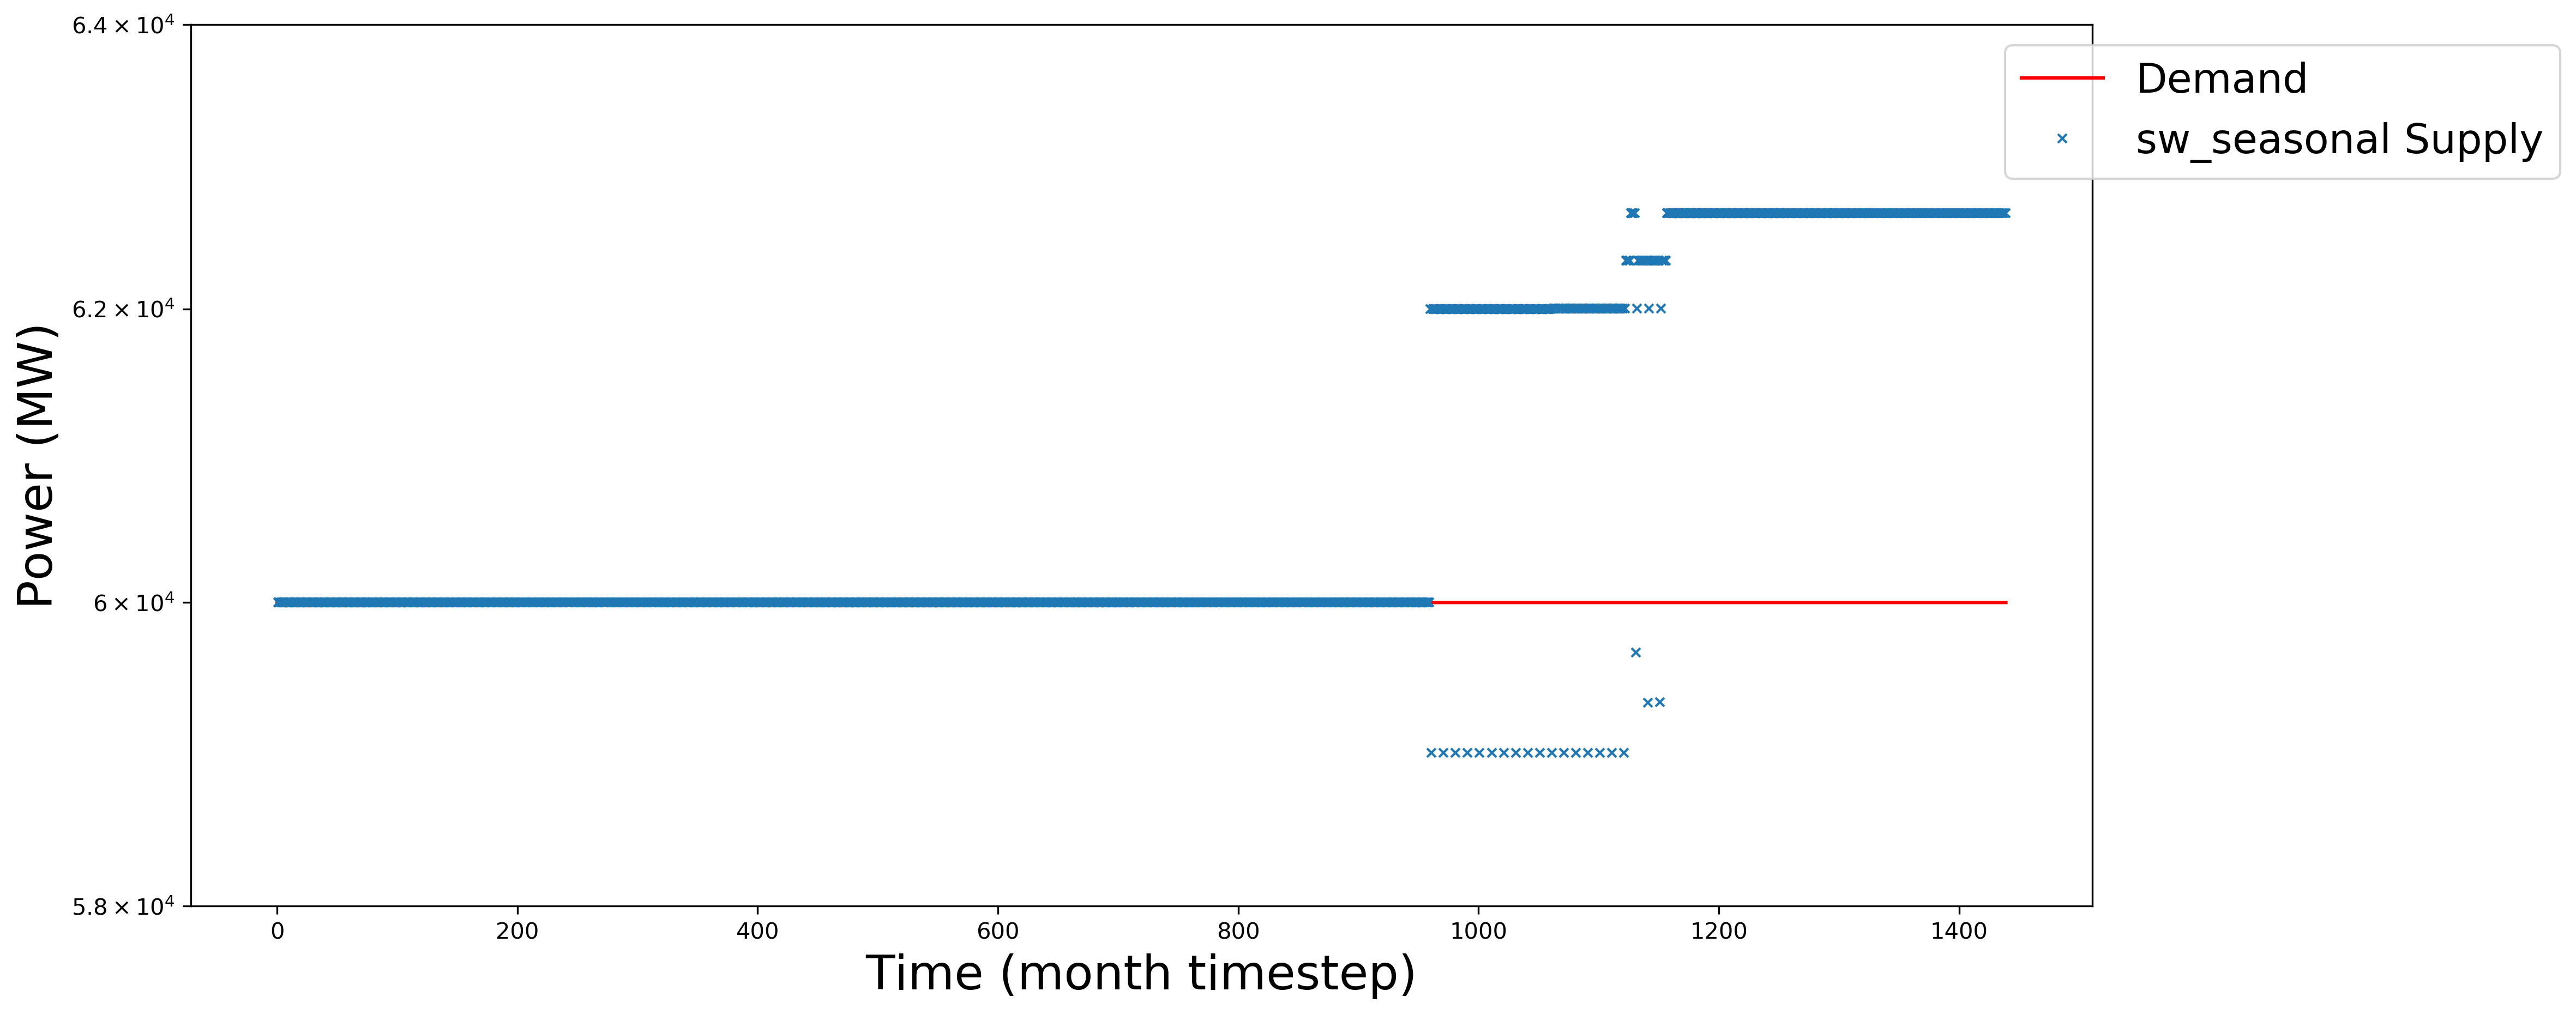
\includegraphics[width=\linewidth]{24-power-bufferB20003.png} 
		\caption{SO algorithms.}
		\label{fig:24powerSO}
\end{subfigure}
	\hfill
	\caption{Plot of the power demand and supply of EG01-EG24 for a constant power demand of 60GW for different prediction algorithms.}
	\label{fig:24power}
\end{figure*}

\subsection{Buffer Size}

This section focuses on the analysis of undersupply dependency on buffer size in the EG01-EG23 transition scenario. Table \ref{tab:buff_size} shows the number of time steps with undersupply and the cumulative undersupply for different buffer sizes and various prediction methods. Figure \ref{buffer_dep} displays the cumulative undersupply as a function of buffer size.

\begin{table}[h]
	\centering
	\caption{Dependency of the undersupply of Power on the buffer size.}
	\label{tab:buff_size}
        \begin{tabularx}{\textwidth}{llcRRRR}
                \hline
        Buffer      &                      & MA   & ARMA  & POLY & EXP       & FFT  \\
        $[MW]$      &                      &      &       &      & SMOOTHING &      \\ \hline
        0             & Undersupplied $[\#]$ & 20   & 60   & 75   & 30             & 28   \\  
                      & Cumulative $[GW]$    & 60.0 & 87.3 & 52.9 & 68.3           & 93.3 \\ \hline
        2000          & Undersupplied $[\#]$ & 20   & 18   & 1    & 20             & 2    \\  
        	      & Cumulative $[GW]$    & 20.0 & 7.7  & 0.3  & 11.0           & 60.3 \\ \hline
        4000          & Undersupplied $[\#]$ & 0    & 0    & 0    & 0              & 1    \\  
	              & Cumulative $[GW]$    & 0    & 0    & 0    & 0              & 60.  \\ \hline
	\end{tabularx}
\end{table}

\begin{figure*}[h!]
	\centering
	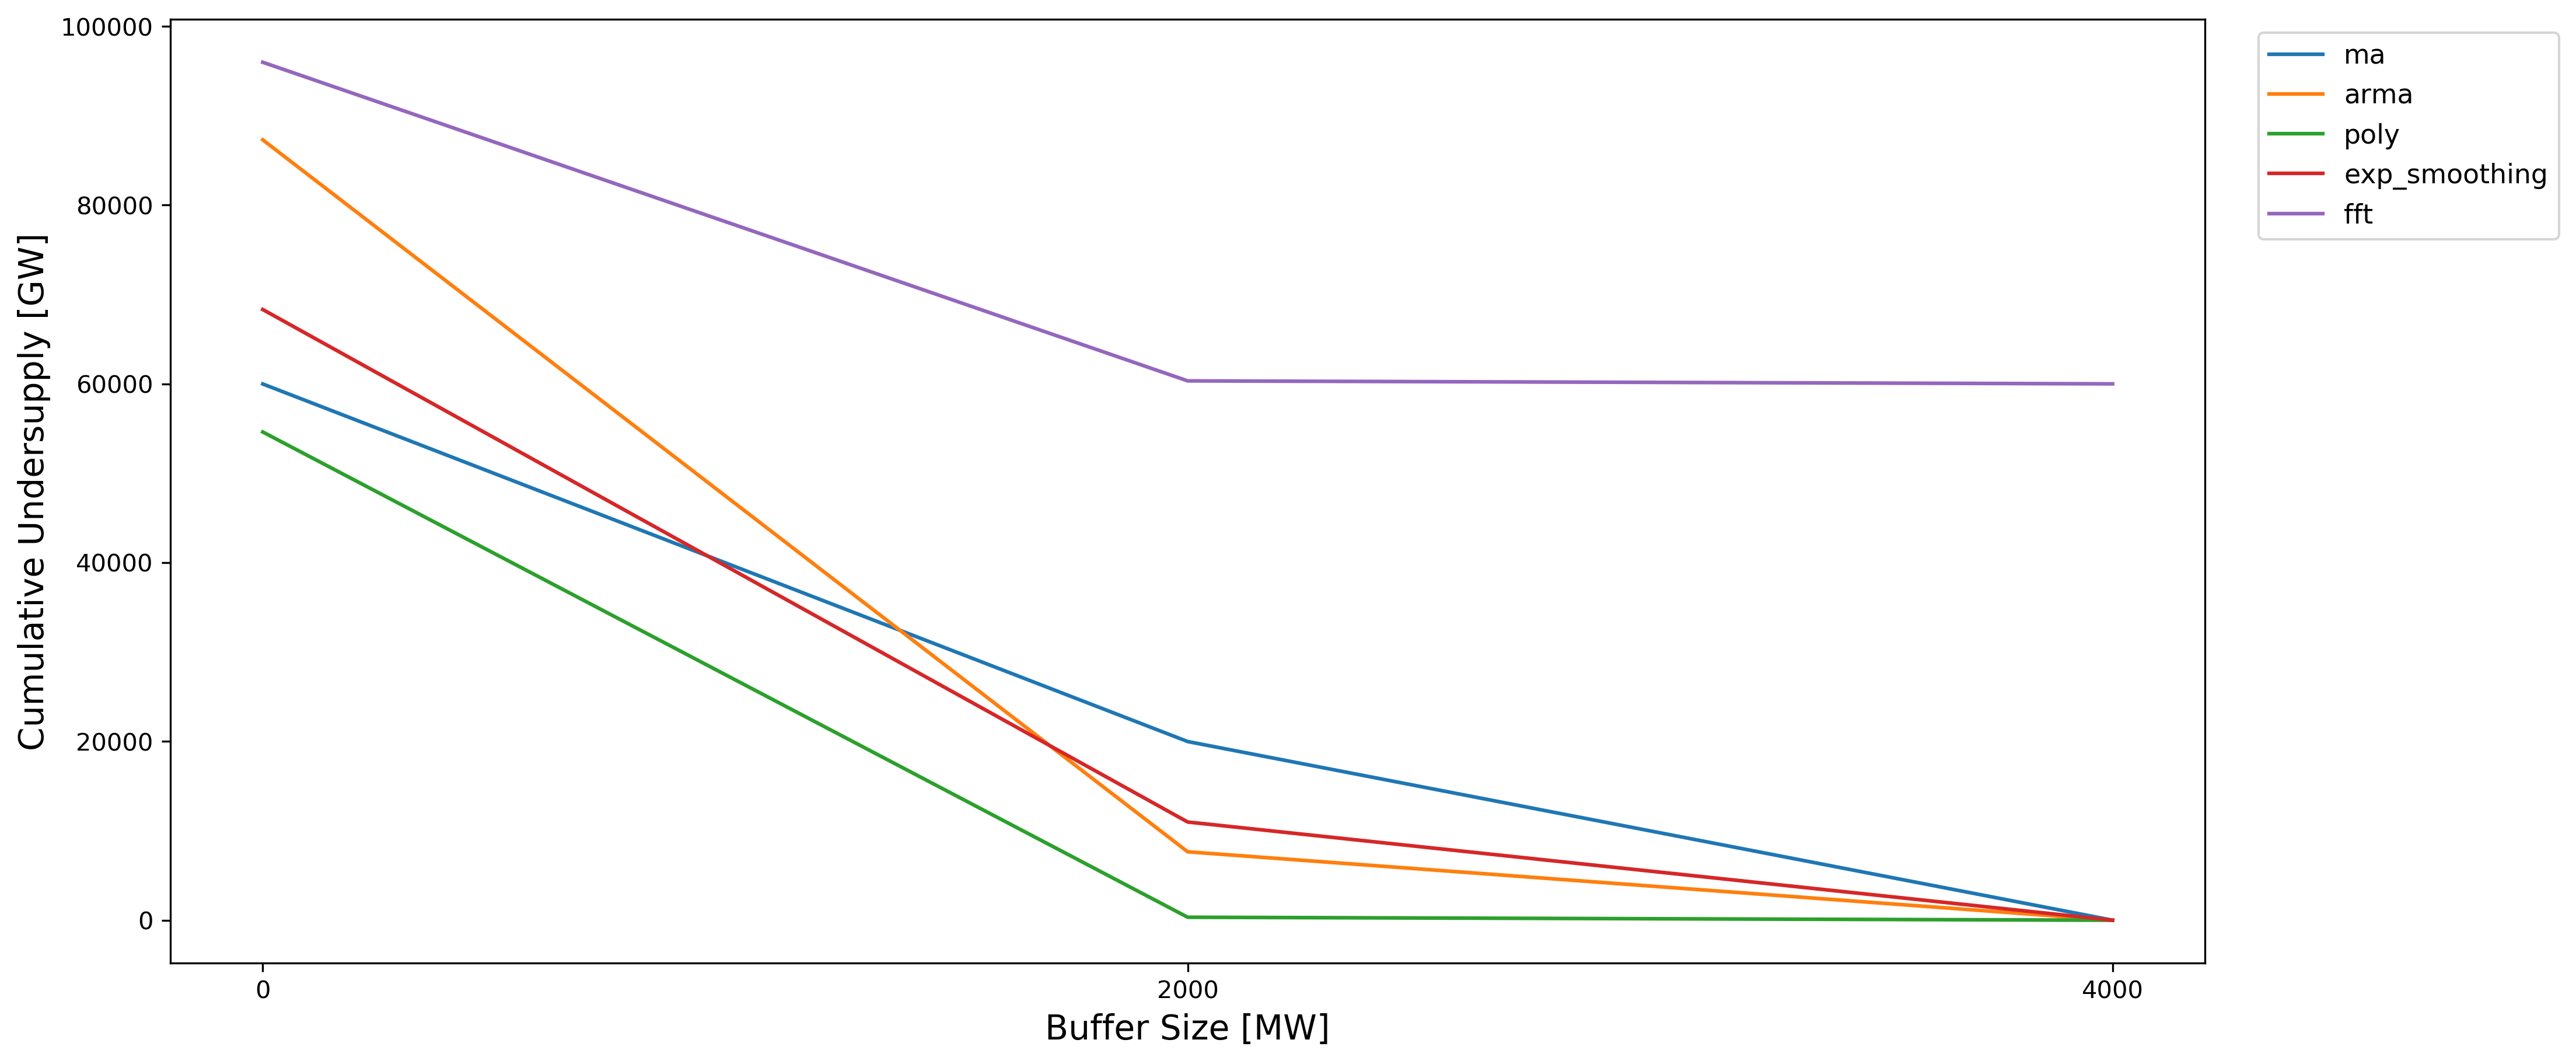
\includegraphics[width=\linewidth]{23-buff.png}
	\caption{Plot of the dependency of the undersupply of Power on the buffer size.}
	\label{buffer_dep}
\end{figure*}

\subsection{Number of Forward Steps}

This section focuses on the dependency on the number of forward steps 
calculated at each time step by the prediction methods in scenario EG01-EG23; 
the buffer size was fixed at 2000 MW. Table \ref{tab:for_steps} shows number of 
time steps containing undersupply and the cumulative undersupply for different 
forward steps for some of the prediction methods. Figure \ref{for_dep} displays 
the cumulative undersupply as a function of the number of forward steps.

\begin{table}[!htbp]
	\centering
	\caption {Dependency of the undersupply of Power on the number of forward steps.}
	\label{tab:for_steps}
        \begin{tabularx}{\textwidth}{llcRRRR}
		\hline
                Forward   &                     & MA   & ARMA & POLY & EXP       & FFT  \\ 
                steps     &                     &      &      &      & SMOOTHING &  \\ \hline
                1         & $\#$ Undersupplied  & 18   & 20   & 2    & 20        & 1   \\  
                          & Cumulative $[GW]$   & 7.6  & 11.0 & 60.3 & 20.0      & 0.3 \\ \hline
                3         & $\#$ Undersupplied  & 1    & 20   & 2    & 0         & 1    \\  
                          & Cumulative $[GW]$   & 0.3  & 11.0 & 60.3 & 0         & 0.3 \\ \hline
                5         & $\#$ Undersupplied  & 4    & 20   & 20   & 0         & 1    \\  
                          & Cumulative $[GW]$   & 1.3  & 11.0 & 60.3 & 0         & 0.3  \\ \hline
	\end{tabularx}
\end{table}

\begin{figure*}[h!]
	\centering
	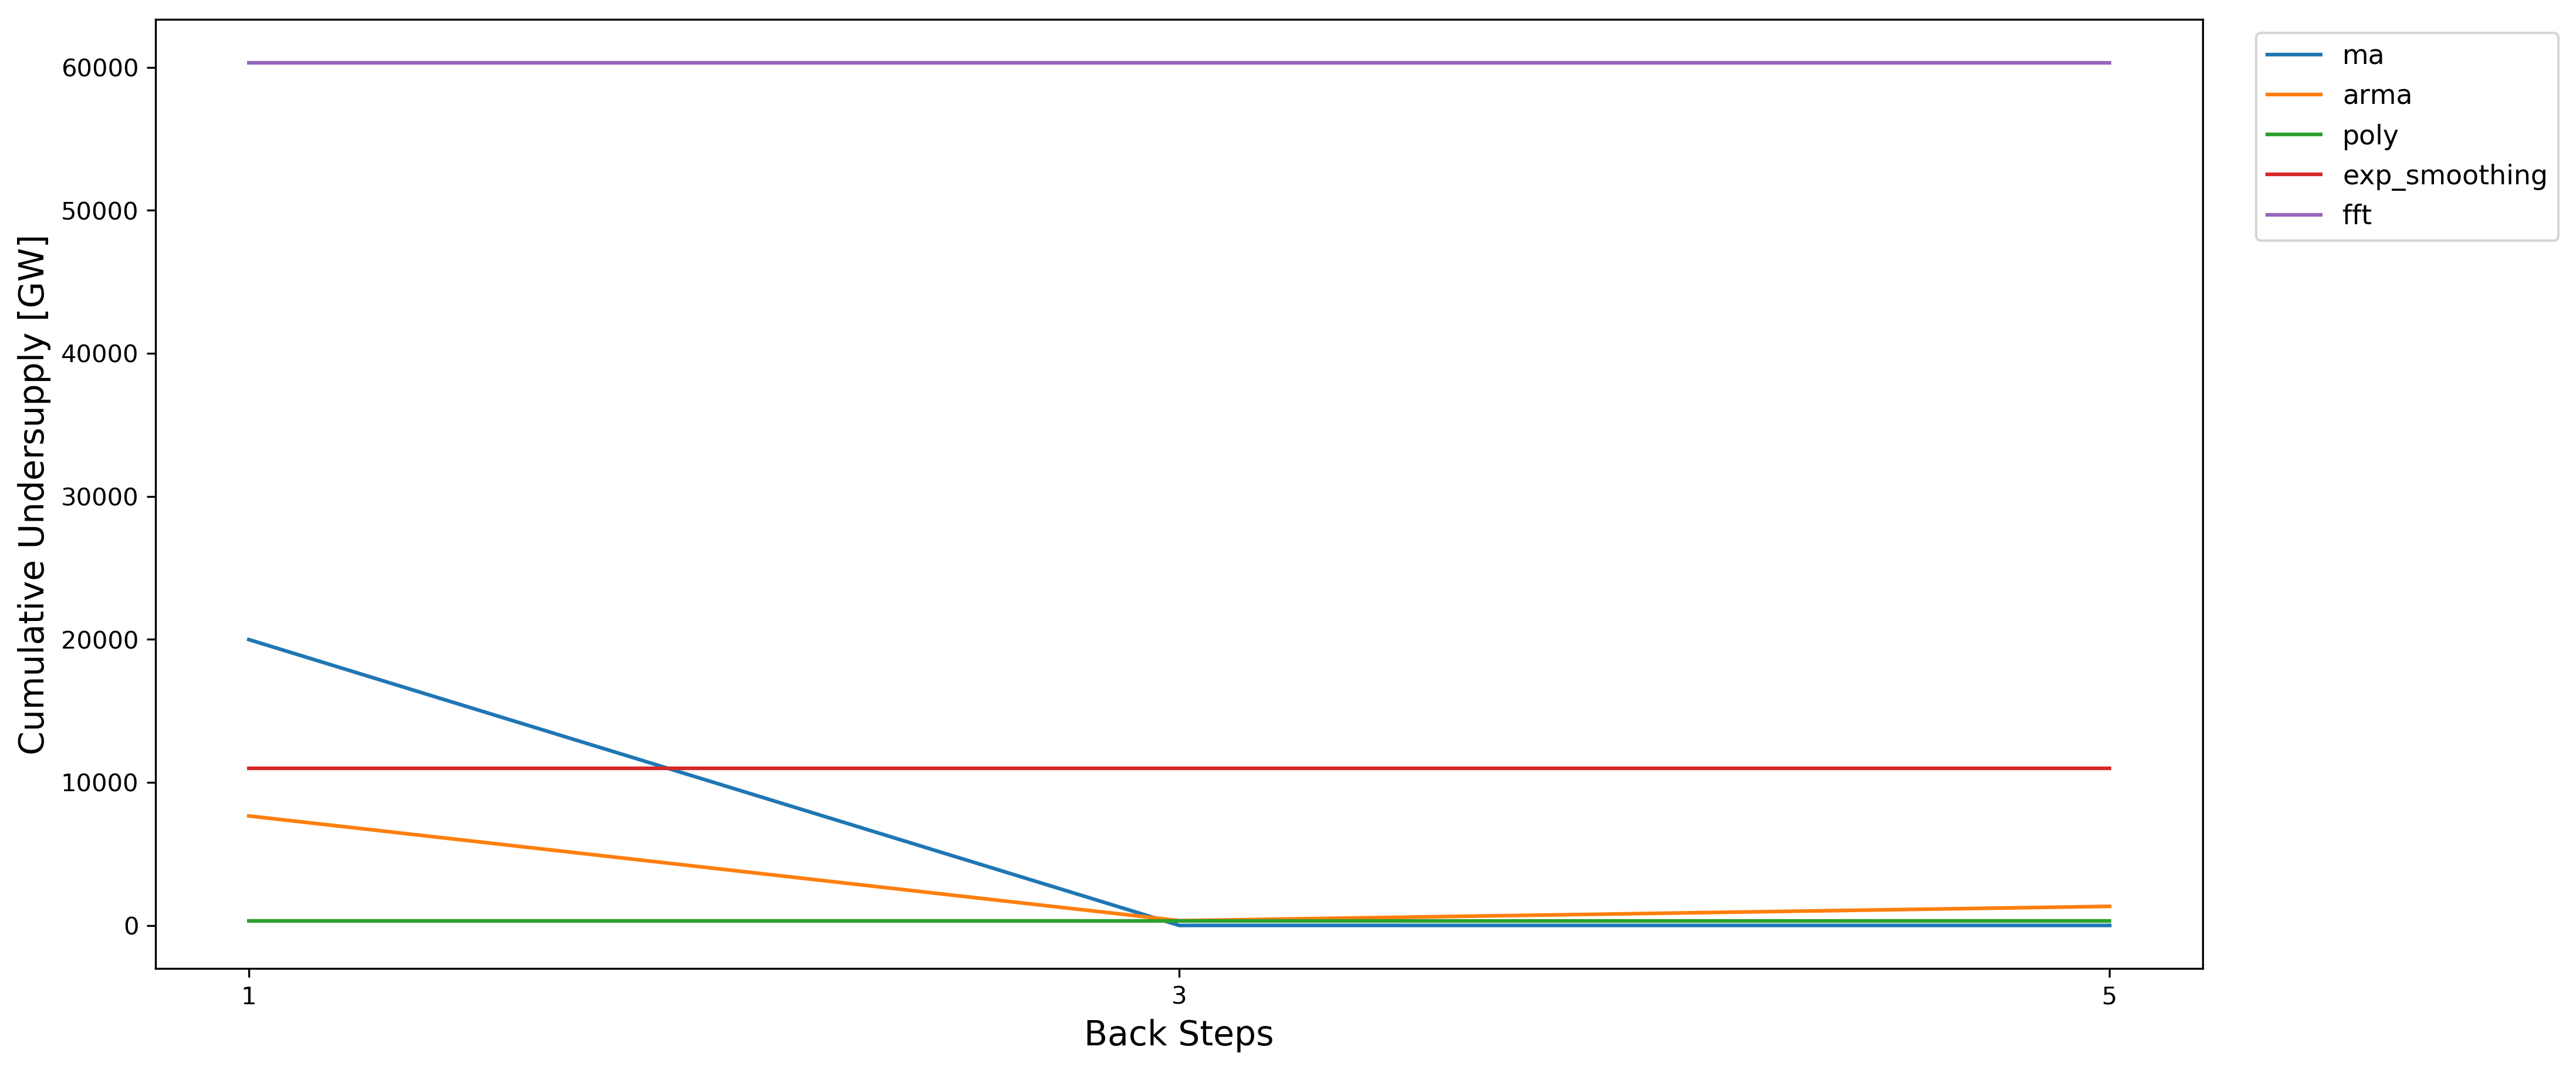
\includegraphics[width=\linewidth]{23-for.png}
	\caption{Plot of the dependency of the undersupply of Power on the 
        number of forward steps.}
	\label{for_dep}
\end{figure*}

\section{Conclusion and Next Steps}
This paper describes the capabilities of \deploy and demonstrates 
the use of \deploy for simple transition scenarios with 
constant, linearly increasing, and sinusoidal power demand.
The demonstration goes further with the more complex transition
scenarios EG01-EG23 and EG01-EG24. This paper also provides insights on
parameter inputs to ease the setup of larger transition scenarios
that may include numerous facilities.

Future work includes setup of similar power demand transition 
scenarios for extended nuclear fuel cycles incorporating multiple reactor designs that consequently use different types of fuel. Such cases are 
currently under study. \cite{wigeland_nuclear_2014} established the transition
scenarios EG01-EG29 and EG01-EG30. These scenarios are more complex than the
cases presented in this report and the distribution of fuel between different
reactor technologies play a main role in the transition.
Additionally, as seen during the demonstration of \deploy capabilities, a Decommissioning capability is highly useful for the setup of several NFCs and is currently under development.

\section{Acknowledgements}
This research is being performed using funding received from the \gls{DOE} Office of 
Nuclear Energy's Nuclear Energy University Program (Project 16-10512, 
DE-NE0008567) 'Demand-Driven Cycamore Archetypes'.

The authors would like to thank 
members of the \gls{ARFC} group at the University of Illinois at 
Urbana-Champaign. 
We also thank our colleagues from the \Cyclus community, 
particularly those in the University of Wisconsin 
\gls{CNERG} and the University of South Carolina Energy Research 
Group (ERGS) for collaborative \Cyclus development.
%----------------------------------------------------------------%

\pagebreak 
\bibliographystyle{plain}
\bibliography{bibliography}

\end{document}


